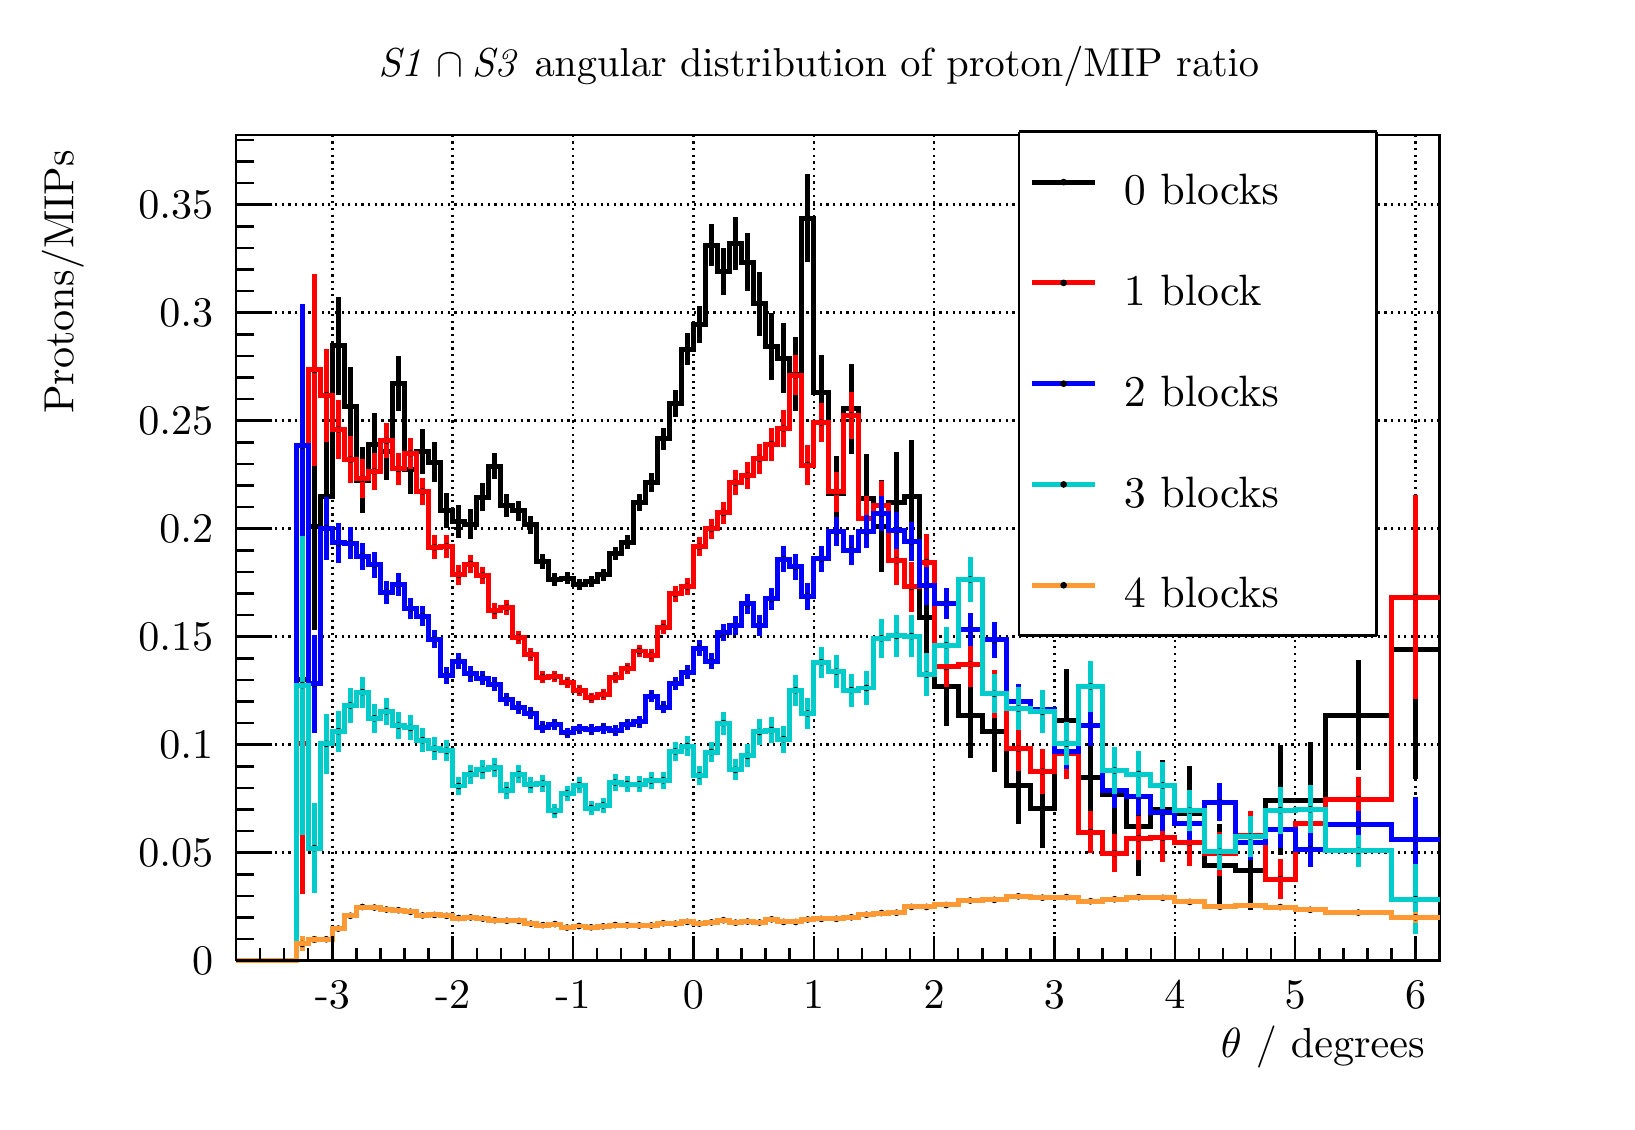
\begin{tikzpicture}
\pgfdeclareplotmark{cross} {
\pgfpathmoveto{\pgfpoint{-0.3\pgfplotmarksize}{\pgfplotmarksize}}
\pgfpathlineto{\pgfpoint{+0.3\pgfplotmarksize}{\pgfplotmarksize}}
\pgfpathlineto{\pgfpoint{+0.3\pgfplotmarksize}{0.3\pgfplotmarksize}}
\pgfpathlineto{\pgfpoint{+1\pgfplotmarksize}{0.3\pgfplotmarksize}}
\pgfpathlineto{\pgfpoint{+1\pgfplotmarksize}{-0.3\pgfplotmarksize}}
\pgfpathlineto{\pgfpoint{+0.3\pgfplotmarksize}{-0.3\pgfplotmarksize}}
\pgfpathlineto{\pgfpoint{+0.3\pgfplotmarksize}{-1.\pgfplotmarksize}}
\pgfpathlineto{\pgfpoint{-0.3\pgfplotmarksize}{-1.\pgfplotmarksize}}
\pgfpathlineto{\pgfpoint{-0.3\pgfplotmarksize}{-0.3\pgfplotmarksize}}
\pgfpathlineto{\pgfpoint{-1.\pgfplotmarksize}{-0.3\pgfplotmarksize}}
\pgfpathlineto{\pgfpoint{-1.\pgfplotmarksize}{0.3\pgfplotmarksize}}
\pgfpathlineto{\pgfpoint{-0.3\pgfplotmarksize}{0.3\pgfplotmarksize}}
\pgfpathclose
\pgfusepathqstroke
}
\pgfdeclareplotmark{cross*} {
\pgfpathmoveto{\pgfpoint{-0.3\pgfplotmarksize}{\pgfplotmarksize}}
\pgfpathlineto{\pgfpoint{+0.3\pgfplotmarksize}{\pgfplotmarksize}}
\pgfpathlineto{\pgfpoint{+0.3\pgfplotmarksize}{0.3\pgfplotmarksize}}
\pgfpathlineto{\pgfpoint{+1\pgfplotmarksize}{0.3\pgfplotmarksize}}
\pgfpathlineto{\pgfpoint{+1\pgfplotmarksize}{-0.3\pgfplotmarksize}}
\pgfpathlineto{\pgfpoint{+0.3\pgfplotmarksize}{-0.3\pgfplotmarksize}}
\pgfpathlineto{\pgfpoint{+0.3\pgfplotmarksize}{-1.\pgfplotmarksize}}
\pgfpathlineto{\pgfpoint{-0.3\pgfplotmarksize}{-1.\pgfplotmarksize}}
\pgfpathlineto{\pgfpoint{-0.3\pgfplotmarksize}{-0.3\pgfplotmarksize}}
\pgfpathlineto{\pgfpoint{-1.\pgfplotmarksize}{-0.3\pgfplotmarksize}}
\pgfpathlineto{\pgfpoint{-1.\pgfplotmarksize}{0.3\pgfplotmarksize}}
\pgfpathlineto{\pgfpoint{-0.3\pgfplotmarksize}{0.3\pgfplotmarksize}}
\pgfpathclose
\pgfusepathqfillstroke
}
\pgfdeclareplotmark{newstar} {
\pgfpathmoveto{\pgfqpoint{0pt}{\pgfplotmarksize}}
\pgfpathlineto{\pgfqpointpolar{44}{0.5\pgfplotmarksize}}
\pgfpathlineto{\pgfqpointpolar{18}{\pgfplotmarksize}}
\pgfpathlineto{\pgfqpointpolar{-20}{0.5\pgfplotmarksize}}
\pgfpathlineto{\pgfqpointpolar{-54}{\pgfplotmarksize}}
\pgfpathlineto{\pgfqpointpolar{-90}{0.5\pgfplotmarksize}}
\pgfpathlineto{\pgfqpointpolar{234}{\pgfplotmarksize}}
\pgfpathlineto{\pgfqpointpolar{198}{0.5\pgfplotmarksize}}
\pgfpathlineto{\pgfqpointpolar{162}{\pgfplotmarksize}}
\pgfpathlineto{\pgfqpointpolar{134}{0.5\pgfplotmarksize}}
\pgfpathclose
\pgfusepathqstroke
}
\pgfdeclareplotmark{newstar*} {
\pgfpathmoveto{\pgfqpoint{0pt}{\pgfplotmarksize}}
\pgfpathlineto{\pgfqpointpolar{44}{0.5\pgfplotmarksize}}
\pgfpathlineto{\pgfqpointpolar{18}{\pgfplotmarksize}}
\pgfpathlineto{\pgfqpointpolar{-20}{0.5\pgfplotmarksize}}
\pgfpathlineto{\pgfqpointpolar{-54}{\pgfplotmarksize}}
\pgfpathlineto{\pgfqpointpolar{-90}{0.5\pgfplotmarksize}}
\pgfpathlineto{\pgfqpointpolar{234}{\pgfplotmarksize}}
\pgfpathlineto{\pgfqpointpolar{198}{0.5\pgfplotmarksize}}
\pgfpathlineto{\pgfqpointpolar{162}{\pgfplotmarksize}}
\pgfpathlineto{\pgfqpointpolar{134}{0.5\pgfplotmarksize}}
\pgfpathclose
\pgfusepathqfillstroke
}
\definecolor{c}{rgb}{1,1,1};
\draw [color=c, fill=c] (0,0) rectangle (20,13.6286);
\draw [color=c, fill=c] (2.6,1.78641) rectangle (17.8857,12.2744);
\definecolor{c}{rgb}{0,0,0};
\draw [c,line width=0.9] (2.6,1.78641) -- (2.6,12.2744) -- (17.8857,12.2744) -- (17.8857,1.78641) -- (2.6,1.78641);
\definecolor{c}{rgb}{1,1,1};
\draw [color=c, fill=c] (2.6,1.78641) rectangle (17.8857,12.2744);
\definecolor{c}{rgb}{0,0,0};
\draw [c,line width=0.9] (2.6,1.78641) -- (2.6,12.2744) -- (17.8857,12.2744) -- (17.8857,1.78641) -- (2.6,1.78641);
\draw [c,line width=0.9] (2.6,1.78641) -- (17.8857,1.78641);
\draw [c,dash pattern=on 0.80pt off 1.60pt ,line width=0.9] (3.82286,12.2744) -- (3.82286,1.78641);
\draw [c,dash pattern=on 0.80pt off 1.60pt ,line width=0.9] (5.35143,12.2744) -- (5.35143,1.78641);
\draw [c,dash pattern=on 0.80pt off 1.60pt ,line width=0.9] (6.88,12.2744) -- (6.88,1.78641);
\draw [c,dash pattern=on 0.80pt off 1.60pt ,line width=0.9] (8.40857,12.2744) -- (8.40857,1.78641);
\draw [c,dash pattern=on 0.80pt off 1.60pt ,line width=0.9] (9.93714,12.2744) -- (9.93714,1.78641);
\draw [c,dash pattern=on 0.80pt off 1.60pt ,line width=0.9] (11.4657,12.2744) -- (11.4657,1.78641);
\draw [c,dash pattern=on 0.80pt off 1.60pt ,line width=0.9] (12.9943,12.2744) -- (12.9943,1.78641);
\draw [c,dash pattern=on 0.80pt off 1.60pt ,line width=0.9] (14.5229,12.2744) -- (14.5229,1.78641);
\draw [c,dash pattern=on 0.80pt off 1.60pt ,line width=0.9] (16.0514,12.2744) -- (16.0514,1.78641);
\draw [c,dash pattern=on 0.80pt off 1.60pt ,line width=0.9] (17.58,12.2744) -- (17.58,1.78641);
\draw [c,dash pattern=on 0.80pt off 1.60pt ,line width=0.9] (3.82286,12.2744) -- (3.82286,1.78641);
\draw [c,dash pattern=on 0.80pt off 1.60pt ,line width=0.9] (17.58,12.2744) -- (17.58,1.78641);
\draw [c,line width=0.9] (2.6,1.78641) -- (2.6,12.2744);
\draw [c,dash pattern=on 0.80pt off 1.60pt ,line width=0.9] (17.8857,1.78641) -- (2.6,1.78641);
\draw [c,dash pattern=on 0.80pt off 1.60pt ,line width=0.9] (17.8857,3.15803) -- (2.6,3.15803);
\draw [c,dash pattern=on 0.80pt off 1.60pt ,line width=0.9] (17.8857,4.52964) -- (2.6,4.52964);
\draw [c,dash pattern=on 0.80pt off 1.60pt ,line width=0.9] (17.8857,5.90126) -- (2.6,5.90126);
\draw [c,dash pattern=on 0.80pt off 1.60pt ,line width=0.9] (17.8857,7.27288) -- (2.6,7.27288);
\draw [c,dash pattern=on 0.80pt off 1.60pt ,line width=0.9] (17.8857,8.64449) -- (2.6,8.64449);
\draw [c,dash pattern=on 0.80pt off 1.60pt ,line width=0.9] (17.8857,10.0161) -- (2.6,10.0161);
\draw [c,dash pattern=on 0.80pt off 1.60pt ,line width=0.9] (17.8857,11.3877) -- (2.6,11.3877);
\draw [c,dash pattern=on 0.80pt off 1.60pt ,line width=0.9] (17.8857,11.3877) -- (2.6,11.3877);
\definecolor{c}{rgb}{0,0,0.6};
\draw [c,line width=0.9] (2.6,1.78641) -- (2.75286,1.78641) -- (2.75286,1.78641) -- (2.90571,1.78641) -- (2.90571,1.78641) -- (3.05857,1.78641) -- (3.05857,1.78641) -- (3.21143,1.78641) -- (3.21143,1.78641) -- (3.36429,1.78641) -- (3.36429,1.78641)
 -- (3.51714,1.78641) -- (3.51714,1.78641) -- (3.67,1.78641) -- (3.67,1.78641) -- (3.82286,1.78641) -- (3.82286,1.78641) -- (3.97571,1.78641) -- (3.97571,1.78641) -- (4.12857,1.78641) -- (4.12857,1.78641) -- (4.28143,1.78641) -- (4.28143,1.78641) --
 (4.43429,1.78641) -- (4.43429,1.78641) -- (4.58714,1.78641) -- (4.58714,1.78641) -- (4.74,1.78641) -- (4.74,1.78641) -- (4.89286,1.78641) -- (4.89286,1.78641) -- (5.04571,1.78641) -- (5.04571,1.78641) -- (5.19857,1.78641) -- (5.19857,1.78641) --
 (5.35143,1.78641) -- (5.35143,1.78641) -- (5.50429,1.78641) -- (5.50429,1.78641) -- (5.65714,1.78641) -- (5.65714,1.78641) -- (5.81,1.78641) -- (5.81,1.78641) -- (5.96286,1.78641) -- (5.96286,1.78641) -- (6.11571,1.78641) -- (6.11571,1.78641) --
 (6.26857,1.78641) -- (6.26857,1.78641) -- (6.42143,1.78641) -- (6.42143,1.78641) -- (6.57429,1.78641) -- (6.57429,1.78641) -- (6.72714,1.78641) -- (6.72714,1.78641) -- (6.88,1.78641) -- (6.88,1.78641) -- (7.03286,1.78641) -- (7.03286,1.78641) --
 (7.18571,1.78641) -- (7.18571,1.78641) -- (7.33857,1.78641) -- (7.33857,1.78641) -- (7.49143,1.78641) -- (7.49143,1.78641) -- (7.64429,1.78641) -- (7.64429,1.78641) -- (7.79714,1.78641) -- (7.79714,1.78641) -- (7.95,1.78641) -- (7.95,1.78641) --
 (8.10286,1.78641) -- (8.10286,1.78641) -- (8.25571,1.78641) -- (8.25571,1.78641) -- (8.40857,1.78641) -- (8.40857,1.78641) -- (8.56143,1.78641) -- (8.56143,1.78641) -- (8.71429,1.78641) -- (8.71429,1.78641) -- (8.86714,1.78641) -- (8.86714,1.78641)
 -- (9.02,1.78641) -- (9.02,1.78641) -- (9.17286,1.78641) -- (9.17286,1.78641) -- (9.32571,1.78641) -- (9.32571,1.78641) -- (9.47857,1.78641) -- (9.47857,1.78641) -- (9.63143,1.78641) -- (9.63143,1.78641) -- (9.78429,1.78641) -- (9.78429,1.78641) --
 (9.93714,1.78641) -- (9.93714,1.78641) -- (10.1282,1.78641) -- (10.1282,1.78641) -- (10.3193,1.78641) -- (10.3193,1.78641) -- (10.5104,1.78641) -- (10.5104,1.78641) -- (10.7014,1.78641) -- (10.7014,1.78641) -- (10.8925,1.78641) -- (10.8925,1.78641)
 -- (11.0836,1.78641) -- (11.0836,1.78641) -- (11.2746,1.78641) -- (11.2746,1.78641) -- (11.4657,1.78641) -- (11.4657,1.78641) -- (11.7714,1.78641) -- (11.7714,1.78641) -- (12.0771,1.78641) -- (12.0771,1.78641) -- (12.3829,1.78641) --
 (12.3829,1.78641) -- (12.6886,1.78641) -- (12.6886,1.78641) -- (12.9943,1.78641) -- (12.9943,1.78641) -- (13.3,1.78641) -- (13.3,1.78641) -- (13.6057,1.78641) -- (13.6057,1.78641) -- (13.9114,1.78641) -- (13.9114,1.78641) -- (14.2171,1.78641) --
 (14.2171,1.78641) -- (14.5229,1.78641) -- (14.5229,1.78641) -- (14.905,1.78641) -- (14.905,1.78641) -- (15.2871,1.78641) -- (15.2871,1.78641) -- (15.6693,1.78641) -- (15.6693,1.78641) -- (16.0514,1.78641) -- (16.0514,1.78641) -- (16.4336,1.78641) --
 (16.4336,1.78641) -- (17.2743,1.78641) -- (17.2743,1.78641) -- (17.8857,1.78641);
\definecolor{c}{rgb}{0,0,0};
\draw [c,line width=0.9] (2.6,1.78641) -- (17.8857,1.78641);
\draw [c,line width=0.9] (3.82286,2.09889) -- (3.82286,1.78641);
\draw [c,line width=0.9] (4.12857,1.94265) -- (4.12857,1.78641);
\draw [c,line width=0.9] (4.43429,1.94265) -- (4.43429,1.78641);
\draw [c,line width=0.9] (4.74,1.94265) -- (4.74,1.78641);
\draw [c,line width=0.9] (5.04571,1.94265) -- (5.04571,1.78641);
\draw [c,line width=0.9] (5.35143,2.09889) -- (5.35143,1.78641);
\draw [c,line width=0.9] (5.65714,1.94265) -- (5.65714,1.78641);
\draw [c,line width=0.9] (5.96286,1.94265) -- (5.96286,1.78641);
\draw [c,line width=0.9] (6.26857,1.94265) -- (6.26857,1.78641);
\draw [c,line width=0.9] (6.57429,1.94265) -- (6.57429,1.78641);
\draw [c,line width=0.9] (6.88,2.09889) -- (6.88,1.78641);
\draw [c,line width=0.9] (7.18571,1.94265) -- (7.18571,1.78641);
\draw [c,line width=0.9] (7.49143,1.94265) -- (7.49143,1.78641);
\draw [c,line width=0.9] (7.79714,1.94265) -- (7.79714,1.78641);
\draw [c,line width=0.9] (8.10286,1.94265) -- (8.10286,1.78641);
\draw [c,line width=0.9] (8.40857,2.09889) -- (8.40857,1.78641);
\draw [c,line width=0.9] (8.71429,1.94265) -- (8.71429,1.78641);
\draw [c,line width=0.9] (9.02,1.94265) -- (9.02,1.78641);
\draw [c,line width=0.9] (9.32571,1.94265) -- (9.32571,1.78641);
\draw [c,line width=0.9] (9.63143,1.94265) -- (9.63143,1.78641);
\draw [c,line width=0.9] (9.93714,2.09889) -- (9.93714,1.78641);
\draw [c,line width=0.9] (10.2429,1.94265) -- (10.2429,1.78641);
\draw [c,line width=0.9] (10.5486,1.94265) -- (10.5486,1.78641);
\draw [c,line width=0.9] (10.8543,1.94265) -- (10.8543,1.78641);
\draw [c,line width=0.9] (11.16,1.94265) -- (11.16,1.78641);
\draw [c,line width=0.9] (11.4657,2.09889) -- (11.4657,1.78641);
\draw [c,line width=0.9] (11.7714,1.94265) -- (11.7714,1.78641);
\draw [c,line width=0.9] (12.0771,1.94265) -- (12.0771,1.78641);
\draw [c,line width=0.9] (12.3829,1.94265) -- (12.3829,1.78641);
\draw [c,line width=0.9] (12.6886,1.94265) -- (12.6886,1.78641);
\draw [c,line width=0.9] (12.9943,2.09889) -- (12.9943,1.78641);
\draw [c,line width=0.9] (13.3,1.94265) -- (13.3,1.78641);
\draw [c,line width=0.9] (13.6057,1.94265) -- (13.6057,1.78641);
\draw [c,line width=0.9] (13.9114,1.94265) -- (13.9114,1.78641);
\draw [c,line width=0.9] (14.2171,1.94265) -- (14.2171,1.78641);
\draw [c,line width=0.9] (14.5229,2.09889) -- (14.5229,1.78641);
\draw [c,line width=0.9] (14.8286,1.94265) -- (14.8286,1.78641);
\draw [c,line width=0.9] (15.1343,1.94265) -- (15.1343,1.78641);
\draw [c,line width=0.9] (15.44,1.94265) -- (15.44,1.78641);
\draw [c,line width=0.9] (15.7457,1.94265) -- (15.7457,1.78641);
\draw [c,line width=0.9] (16.0514,2.09889) -- (16.0514,1.78641);
\draw [c,line width=0.9] (16.3571,1.94265) -- (16.3571,1.78641);
\draw [c,line width=0.9] (16.6629,1.94265) -- (16.6629,1.78641);
\draw [c,line width=0.9] (16.9686,1.94265) -- (16.9686,1.78641);
\draw [c,line width=0.9] (17.2743,1.94265) -- (17.2743,1.78641);
\draw [c,line width=0.9] (17.58,2.09889) -- (17.58,1.78641);
\draw [c,line width=0.9] (3.82286,2.09889) -- (3.82286,1.78641);
\draw [c,line width=0.9] (3.51714,1.94265) -- (3.51714,1.78641);
\draw [c,line width=0.9] (3.21143,1.94265) -- (3.21143,1.78641);
\draw [c,line width=0.9] (2.90571,1.94265) -- (2.90571,1.78641);
\draw [c,line width=0.9] (17.58,2.09889) -- (17.58,1.78641);
\draw [anchor=base] (3.82286,1.17312) node[scale=1.52295, color=c, rotate=0]{-3};
\draw [anchor=base] (5.35143,1.17312) node[scale=1.52295, color=c, rotate=0]{-2};
\draw [anchor=base] (6.88,1.17312) node[scale=1.52295, color=c, rotate=0]{-1};
\draw [anchor=base] (8.40857,1.17312) node[scale=1.52295, color=c, rotate=0]{0};
\draw [anchor=base] (9.93714,1.17312) node[scale=1.52295, color=c, rotate=0]{1};
\draw [anchor=base] (11.4657,1.17312) node[scale=1.52295, color=c, rotate=0]{2};
\draw [anchor=base] (12.9943,1.17312) node[scale=1.52295, color=c, rotate=0]{3};
\draw [anchor=base] (14.5229,1.17312) node[scale=1.52295, color=c, rotate=0]{4};
\draw [anchor=base] (16.0514,1.17312) node[scale=1.52295, color=c, rotate=0]{5};
\draw [anchor=base] (17.58,1.17312) node[scale=1.52295, color=c, rotate=0]{6};
\draw [anchor= east] (17.8857,0.696123) node[scale=1.52295, color=c, rotate=0]{$\theta$ / degrees};
\draw [c,line width=0.9] (2.6,1.78641) -- (2.6,12.2744);
\draw [c,line width=0.9] (3.06173,1.78641) -- (2.6,1.78641);
\draw [c,line width=0.9] (2.83087,2.06073) -- (2.6,2.06073);
\draw [c,line width=0.9] (2.83087,2.33506) -- (2.6,2.33506);
\draw [c,line width=0.9] (2.83087,2.60938) -- (2.6,2.60938);
\draw [c,line width=0.9] (2.83087,2.8837) -- (2.6,2.8837);
\draw [c,line width=0.9] (3.06173,3.15803) -- (2.6,3.15803);
\draw [c,line width=0.9] (2.83087,3.43235) -- (2.6,3.43235);
\draw [c,line width=0.9] (2.83087,3.70667) -- (2.6,3.70667);
\draw [c,line width=0.9] (2.83087,3.981) -- (2.6,3.981);
\draw [c,line width=0.9] (2.83087,4.25532) -- (2.6,4.25532);
\draw [c,line width=0.9] (3.06173,4.52964) -- (2.6,4.52964);
\draw [c,line width=0.9] (2.83087,4.80397) -- (2.6,4.80397);
\draw [c,line width=0.9] (2.83087,5.07829) -- (2.6,5.07829);
\draw [c,line width=0.9] (2.83087,5.35261) -- (2.6,5.35261);
\draw [c,line width=0.9] (2.83087,5.62694) -- (2.6,5.62694);
\draw [c,line width=0.9] (3.06173,5.90126) -- (2.6,5.90126);
\draw [c,line width=0.9] (2.83087,6.17558) -- (2.6,6.17558);
\draw [c,line width=0.9] (2.83087,6.44991) -- (2.6,6.44991);
\draw [c,line width=0.9] (2.83087,6.72423) -- (2.6,6.72423);
\draw [c,line width=0.9] (2.83087,6.99855) -- (2.6,6.99855);
\draw [c,line width=0.9] (3.06173,7.27288) -- (2.6,7.27288);
\draw [c,line width=0.9] (2.83087,7.5472) -- (2.6,7.5472);
\draw [c,line width=0.9] (2.83087,7.82152) -- (2.6,7.82152);
\draw [c,line width=0.9] (2.83087,8.09585) -- (2.6,8.09585);
\draw [c,line width=0.9] (2.83087,8.37017) -- (2.6,8.37017);
\draw [c,line width=0.9] (3.06173,8.64449) -- (2.6,8.64449);
\draw [c,line width=0.9] (2.83087,8.91882) -- (2.6,8.91882);
\draw [c,line width=0.9] (2.83087,9.19314) -- (2.6,9.19314);
\draw [c,line width=0.9] (2.83087,9.46746) -- (2.6,9.46746);
\draw [c,line width=0.9] (2.83087,9.74179) -- (2.6,9.74179);
\draw [c,line width=0.9] (3.06173,10.0161) -- (2.6,10.0161);
\draw [c,line width=0.9] (2.83087,10.2904) -- (2.6,10.2904);
\draw [c,line width=0.9] (2.83087,10.5648) -- (2.6,10.5648);
\draw [c,line width=0.9] (2.83087,10.8391) -- (2.6,10.8391);
\draw [c,line width=0.9] (2.83087,11.1134) -- (2.6,11.1134);
\draw [c,line width=0.9] (3.06173,11.3877) -- (2.6,11.3877);
\draw [c,line width=0.9] (3.06173,11.3877) -- (2.6,11.3877);
\draw [c,line width=0.9] (2.83087,11.6621) -- (2.6,11.6621);
\draw [c,line width=0.9] (2.83087,11.9364) -- (2.6,11.9364);
\draw [c,line width=0.9] (2.83087,12.2107) -- (2.6,12.2107);
\draw [anchor= east] (2.5,1.78641) node[scale=1.52295, color=c, rotate=0]{0};
\draw [anchor= east] (2.5,3.15803) node[scale=1.52295, color=c, rotate=0]{0.05};
\draw [anchor= east] (2.5,4.52964) node[scale=1.52295, color=c, rotate=0]{0.1};
\draw [anchor= east] (2.5,5.90126) node[scale=1.52295, color=c, rotate=0]{0.15};
\draw [anchor= east] (2.5,7.27288) node[scale=1.52295, color=c, rotate=0]{0.2};
\draw [anchor= east] (2.5,8.64449) node[scale=1.52295, color=c, rotate=0]{0.25};
\draw [anchor= east] (2.5,10.0161) node[scale=1.52295, color=c, rotate=0]{0.3};
\draw [anchor= east] (2.5,11.3877) node[scale=1.52295, color=c, rotate=0]{0.35};
\draw [anchor= east] (0.4,12.2744) node[scale=1.52295, color=c, rotate=90]{  Protons/MIPs};
\draw [c,line width=1.8] (3.44071,3.44162) -- (3.44071,5.3542);
\draw [c,line width=1.8] (3.44071,5.3542) -- (3.44071,7.26677);
\foreach \P in {(3.44071,5.3542)}{\draw[mark options={color=c,fill=c},mark size=2.402402pt,mark=*,mark size=1pt] plot coordinates {\P};}
\draw [c,line width=1.8] (3.59357,5.98089) -- (3.59357,7.30347);
\draw [c,line width=1.8] (3.59357,7.30347) -- (3.59357,8.62605);
\foreach \P in {(3.59357,7.30347)}{\draw[mark options={color=c,fill=c},mark size=2.402402pt,mark=*,mark size=1pt] plot coordinates {\P};}
\draw [c,line width=1.8] (3.74643,6.88782) -- (3.74643,7.6815);
\draw [c,line width=1.8] (3.74643,7.6815) -- (3.74643,8.47519);
\foreach \P in {(3.74643,7.6815)}{\draw[mark options={color=c,fill=c},mark size=2.402402pt,mark=*,mark size=1pt] plot coordinates {\P};}
\draw [c,line width=1.8] (3.89929,8.96737) -- (3.89929,9.59348);
\draw [c,line width=1.8] (3.89929,9.59348) -- (3.89929,10.2196);
\foreach \P in {(3.89929,9.59348)}{\draw[mark options={color=c,fill=c},mark size=2.402402pt,mark=*,mark size=1pt] plot coordinates {\P};}
\draw [c,line width=1.8] (4.05214,8.33148) -- (4.05214,8.82768);
\draw [c,line width=1.8] (4.05214,8.82768) -- (4.05214,9.32388);
\foreach \P in {(4.05214,8.82768)}{\draw[mark options={color=c,fill=c},mark size=2.402402pt,mark=*,mark size=1pt] plot coordinates {\P};}
\draw [c,line width=1.8] (4.205,7.46907) -- (4.205,7.89071);
\draw [c,line width=1.8] (4.205,7.89071) -- (4.205,8.31235);
\foreach \P in {(4.205,7.89071)}{\draw[mark options={color=c,fill=c},mark size=2.402402pt,mark=*,mark size=1pt] plot coordinates {\P};}
\draw [c,line width=1.8] (4.35786,7.95529) -- (4.35786,8.34592);
\draw [c,line width=1.8] (4.35786,8.34592) -- (4.35786,8.73655);
\foreach \P in {(4.35786,8.34592)}{\draw[mark options={color=c,fill=c},mark size=2.402402pt,mark=*,mark size=1pt] plot coordinates {\P};}
\draw [c,line width=1.8] (4.51071,7.88765) -- (4.51071,8.25143);
\draw [c,line width=1.8] (4.51071,8.25143) -- (4.51071,8.6152);
\foreach \P in {(4.51071,8.25143)}{\draw[mark options={color=c,fill=c},mark size=2.402402pt,mark=*,mark size=1pt] plot coordinates {\P};}
\draw [c,line width=1.8] (4.66357,8.77002) -- (4.66357,9.11879);
\draw [c,line width=1.8] (4.66357,9.11879) -- (4.66357,9.46756);
\foreach \P in {(4.66357,9.11879)}{\draw[mark options={color=c,fill=c},mark size=2.402402pt,mark=*,mark size=1pt] plot coordinates {\P};}
\draw [c,line width=1.8] (4.81643,7.71788) -- (4.81643,8.02665);
\draw [c,line width=1.8] (4.81643,8.02665) -- (4.81643,8.33543);
\foreach \P in {(4.81643,8.02665)}{\draw[mark options={color=c,fill=c},mark size=2.402402pt,mark=*,mark size=1pt] plot coordinates {\P};}
\draw [c,line width=1.8] (4.96929,7.96523) -- (4.96929,8.24951);
\draw [c,line width=1.8] (4.96929,8.24951) -- (4.96929,8.53378);
\foreach \P in {(4.96929,8.24951)}{\draw[mark options={color=c,fill=c},mark size=2.402402pt,mark=*,mark size=1pt] plot coordinates {\P};}
\draw [c,line width=1.8] (5.12214,7.8602) -- (5.12214,8.11858);
\draw [c,line width=1.8] (5.12214,8.11858) -- (5.12214,8.37696);
\foreach \P in {(5.12214,8.11858)}{\draw[mark options={color=c,fill=c},mark size=2.402402pt,mark=*,mark size=1pt] plot coordinates {\P};}
\draw [c,line width=1.8] (5.275,7.27724) -- (5.275,7.50472);
\draw [c,line width=1.8] (5.275,7.50472) -- (5.275,7.7322);
\foreach \P in {(5.275,7.50472)}{\draw[mark options={color=c,fill=c},mark size=2.402402pt,mark=*,mark size=1pt] plot coordinates {\P};}
\draw [c,line width=1.8] (5.42786,7.15606) -- (5.42786,7.36413);
\draw [c,line width=1.8] (5.42786,7.36413) -- (5.42786,7.5722);
\foreach \P in {(5.42786,7.36413)}{\draw[mark options={color=c,fill=c},mark size=2.402402pt,mark=*,mark size=1pt] plot coordinates {\P};}
\draw [c,line width=1.8] (5.58071,7.14091) -- (5.58071,7.33025);
\draw [c,line width=1.8] (5.58071,7.33025) -- (5.58071,7.5196);
\foreach \P in {(5.58071,7.33025)}{\draw[mark options={color=c,fill=c},mark size=2.402402pt,mark=*,mark size=1pt] plot coordinates {\P};}
\draw [c,line width=1.8] (5.73357,7.49256) -- (5.73357,7.67138);
\draw [c,line width=1.8] (5.73357,7.67138) -- (5.73357,7.85019);
\foreach \P in {(5.73357,7.67138)}{\draw[mark options={color=c,fill=c},mark size=2.402402pt,mark=*,mark size=1pt] plot coordinates {\P};}
\draw [c,line width=1.8] (5.88643,7.89938) -- (5.88643,8.06413);
\draw [c,line width=1.8] (5.88643,8.06413) -- (5.88643,8.22887);
\foreach \P in {(5.88643,8.06413)}{\draw[mark options={color=c,fill=c},mark size=2.402402pt,mark=*,mark size=1pt] plot coordinates {\P};}
\draw [c,line width=1.8] (6.03929,7.42558) -- (6.03929,7.57121);
\draw [c,line width=1.8] (6.03929,7.57121) -- (6.03929,7.71684);
\foreach \P in {(6.03929,7.57121)}{\draw[mark options={color=c,fill=c},mark size=2.402402pt,mark=*,mark size=1pt] plot coordinates {\P};}
\draw [c,line width=1.8] (6.19214,7.3739) -- (6.19214,7.5013);
\draw [c,line width=1.8] (6.19214,7.5013) -- (6.19214,7.62871);
\foreach \P in {(6.19214,7.5013)}{\draw[mark options={color=c,fill=c},mark size=2.402402pt,mark=*,mark size=1pt] plot coordinates {\P};}
\draw [c,line width=1.8] (6.345,7.21014) -- (6.345,7.32063);
\draw [c,line width=1.8] (6.345,7.32063) -- (6.345,7.43112);
\foreach \P in {(6.345,7.32063)}{\draw[mark options={color=c,fill=c},mark size=2.402402pt,mark=*,mark size=1pt] plot coordinates {\P};}
\draw [c,line width=1.8] (6.49786,6.76574) -- (6.49786,6.85947);
\draw [c,line width=1.8] (6.49786,6.85947) -- (6.49786,6.9532);
\foreach \P in {(6.49786,6.85947)}{\draw[mark options={color=c,fill=c},mark size=2.402402pt,mark=*,mark size=1pt] plot coordinates {\P};}
\draw [c,line width=1.8] (6.65071,6.54051) -- (6.65071,6.62217);
\draw [c,line width=1.8] (6.65071,6.62217) -- (6.65071,6.70382);
\foreach \P in {(6.65071,6.62217)}{\draw[mark options={color=c,fill=c},mark size=2.402402pt,mark=*,mark size=1pt] plot coordinates {\P};}
\draw [c,line width=1.8] (6.80357,6.56641) -- (6.80357,6.642);
\draw [c,line width=1.8] (6.80357,6.642) -- (6.80357,6.71759);
\foreach \P in {(6.80357,6.642)}{\draw[mark options={color=c,fill=c},mark size=2.402402pt,mark=*,mark size=1pt] plot coordinates {\P};}
\draw [c,line width=1.8] (6.95643,6.49565) -- (6.95643,6.56713);
\draw [c,line width=1.8] (6.95643,6.56713) -- (6.95643,6.63862);
\foreach \P in {(6.95643,6.56713)}{\draw[mark options={color=c,fill=c},mark size=2.402402pt,mark=*,mark size=1pt] plot coordinates {\P};}
\draw [c,line width=1.8] (7.10929,6.52617) -- (7.10929,6.59759);
\draw [c,line width=1.8] (7.10929,6.59759) -- (7.10929,6.66901);
\foreach \P in {(7.10929,6.59759)}{\draw[mark options={color=c,fill=c},mark size=2.402402pt,mark=*,mark size=1pt] plot coordinates {\P};}
\draw [c,line width=1.8] (7.26214,6.61085) -- (7.26214,6.68513);
\draw [c,line width=1.8] (7.26214,6.68513) -- (7.26214,6.75942);
\foreach \P in {(7.26214,6.68513)}{\draw[mark options={color=c,fill=c},mark size=2.402402pt,mark=*,mark size=1pt] plot coordinates {\P};}
\draw [c,line width=1.8] (7.415,6.87015) -- (7.415,6.95203);
\draw [c,line width=1.8] (7.415,6.95203) -- (7.415,7.03392);
\foreach \P in {(7.415,6.95203)}{\draw[mark options={color=c,fill=c},mark size=2.402402pt,mark=*,mark size=1pt] plot coordinates {\P};}
\draw [c,line width=1.8] (7.56786,7.01129) -- (7.56786,7.10253);
\draw [c,line width=1.8] (7.56786,7.10253) -- (7.56786,7.19377);
\foreach \P in {(7.56786,7.10253)}{\draw[mark options={color=c,fill=c},mark size=2.402402pt,mark=*,mark size=1pt] plot coordinates {\P};}
\draw [c,line width=1.8] (7.72071,7.49941) -- (7.72071,7.60428);
\draw [c,line width=1.8] (7.72071,7.60428) -- (7.72071,7.70915);
\foreach \P in {(7.72071,7.60428)}{\draw[mark options={color=c,fill=c},mark size=2.402402pt,mark=*,mark size=1pt] plot coordinates {\P};}
\draw [c,line width=1.8] (7.87357,7.74479) -- (7.87357,7.86464);
\draw [c,line width=1.8] (7.87357,7.86464) -- (7.87357,7.98448);
\foreach \P in {(7.87357,7.86464)}{\draw[mark options={color=c,fill=c},mark size=2.402402pt,mark=*,mark size=1pt] plot coordinates {\P};}
\draw [c,line width=1.8] (8.02643,8.26984) -- (8.02643,8.41182);
\draw [c,line width=1.8] (8.02643,8.41182) -- (8.02643,8.55379);
\foreach \P in {(8.02643,8.41182)}{\draw[mark options={color=c,fill=c},mark size=2.402402pt,mark=*,mark size=1pt] plot coordinates {\P};}
\draw [c,line width=1.8] (8.17929,8.69499) -- (8.17929,8.86269);
\draw [c,line width=1.8] (8.17929,8.86269) -- (8.17929,9.0304);
\foreach \P in {(8.17929,8.86269)}{\draw[mark options={color=c,fill=c},mark size=2.402402pt,mark=*,mark size=1pt] plot coordinates {\P};}
\draw [c,line width=1.8] (8.33214,9.34922) -- (8.33214,9.55224);
\draw [c,line width=1.8] (8.33214,9.55224) -- (8.33214,9.75526);
\foreach \P in {(8.33214,9.55224)}{\draw[mark options={color=c,fill=c},mark size=2.402402pt,mark=*,mark size=1pt] plot coordinates {\P};}
\draw [c,line width=1.8] (8.485,9.62913) -- (8.485,9.86622);
\draw [c,line width=1.8] (8.485,9.86622) -- (8.485,10.1033);
\foreach \P in {(8.485,9.86622)}{\draw[mark options={color=c,fill=c},mark size=2.402402pt,mark=*,mark size=1pt] plot coordinates {\P};}
\draw [c,line width=1.8] (8.63786,10.6044) -- (8.63786,10.8736);
\draw [c,line width=1.8] (8.63786,10.8736) -- (8.63786,11.1428);
\foreach \P in {(8.63786,10.8736)}{\draw[mark options={color=c,fill=c},mark size=2.402402pt,mark=*,mark size=1pt] plot coordinates {\P};}
\draw [c,line width=1.8] (8.79071,10.2368) -- (8.79071,10.5384);
\draw [c,line width=1.8] (8.79071,10.5384) -- (8.79071,10.8399);
\foreach \P in {(8.79071,10.5384)}{\draw[mark options={color=c,fill=c},mark size=2.402402pt,mark=*,mark size=1pt] plot coordinates {\P};}
\draw [c,line width=1.8] (8.94357,10.5526) -- (8.94357,10.8931);
\draw [c,line width=1.8] (8.94357,10.8931) -- (8.94357,11.2337);
\foreach \P in {(8.94357,10.8931)}{\draw[mark options={color=c,fill=c},mark size=2.402402pt,mark=*,mark size=1pt] plot coordinates {\P};}
\draw [c,line width=1.8] (9.09643,10.2895) -- (9.09643,10.659);
\draw [c,line width=1.8] (9.09643,10.659) -- (9.09643,11.0285);
\foreach \P in {(9.09643,10.659)}{\draw[mark options={color=c,fill=c},mark size=2.402402pt,mark=*,mark size=1pt] plot coordinates {\P};}
\draw [c,line width=1.8] (9.24929,9.72369) -- (9.24929,10.128);
\draw [c,line width=1.8] (9.24929,10.128) -- (9.24929,10.5323);
\foreach \P in {(9.24929,10.128)}{\draw[mark options={color=c,fill=c},mark size=2.402402pt,mark=*,mark size=1pt] plot coordinates {\P};}
\draw [c,line width=1.8] (9.40214,9.16348) -- (9.40214,9.58824);
\draw [c,line width=1.8] (9.40214,9.58824) -- (9.40214,10.013);
\foreach \P in {(9.40214,9.58824)}{\draw[mark options={color=c,fill=c},mark size=2.402402pt,mark=*,mark size=1pt] plot coordinates {\P};}
\draw [c,line width=1.8] (9.555,8.99626) -- (9.555,9.43778);
\draw [c,line width=1.8] (9.555,9.43778) -- (9.555,9.87931);
\foreach \P in {(9.555,9.43778)}{\draw[mark options={color=c,fill=c},mark size=2.402402pt,mark=*,mark size=1pt] plot coordinates {\P};}
\draw [c,line width=1.8] (9.70786,8.76439) -- (9.70786,9.2371);
\draw [c,line width=1.8] (9.70786,9.2371) -- (9.70786,9.70981);
\foreach \P in {(9.70786,9.2371)}{\draw[mark options={color=c,fill=c},mark size=2.402402pt,mark=*,mark size=1pt] plot coordinates {\P};}
\draw [c,line width=1.8] (9.86071,10.6603) -- (9.86071,11.2176);
\draw [c,line width=1.8] (9.86071,11.2176) -- (9.86071,11.7749);
\foreach \P in {(9.86071,11.2176)}{\draw[mark options={color=c,fill=c},mark size=2.402402pt,mark=*,mark size=1pt] plot coordinates {\P};}
\draw [c,line width=1.8] (10.0327,8.52843) -- (10.0327,9.0016);
\draw [c,line width=1.8] (10.0327,9.0016) -- (10.0327,9.47476);
\foreach \P in {(10.0327,9.0016)}{\draw[mark options={color=c,fill=c},mark size=2.402402pt,mark=*,mark size=1pt] plot coordinates {\P};}
\draw [c,line width=1.8] (10.2238,7.23587) -- (10.2238,7.71335);
\draw [c,line width=1.8] (10.2238,7.71335) -- (10.2238,8.19084);
\foreach \P in {(10.2238,7.71335)}{\draw[mark options={color=c,fill=c},mark size=2.402402pt,mark=*,mark size=1pt] plot coordinates {\P};}
\draw [c,line width=1.8] (10.4148,8.22526) -- (10.4148,8.7943);
\draw [c,line width=1.8] (10.4148,8.7943) -- (10.4148,9.36334);
\foreach \P in {(10.4148,8.7943)}{\draw[mark options={color=c,fill=c},mark size=2.402402pt,mark=*,mark size=1pt] plot coordinates {\P};}
\draw [c,line width=1.8] (10.6059,7.09923) -- (10.6059,7.66068);
\draw [c,line width=1.8] (10.6059,7.66068) -- (10.6059,8.22214);
\foreach \P in {(10.6059,7.66068)}{\draw[mark options={color=c,fill=c},mark size=2.402402pt,mark=*,mark size=1pt] plot coordinates {\P};}
\draw [c,line width=1.8] (10.797,6.72351) -- (10.797,7.30412);
\draw [c,line width=1.8] (10.797,7.30412) -- (10.797,7.88473);
\foreach \P in {(10.797,7.30412)}{\draw[mark options={color=c,fill=c},mark size=2.402402pt,mark=*,mark size=1pt] plot coordinates {\P};}
\draw [c,line width=1.8] (10.988,6.96747) -- (10.988,7.60644);
\draw [c,line width=1.8] (10.988,7.60644) -- (10.988,8.24541);
\foreach \P in {(10.988,7.60644)}{\draw[mark options={color=c,fill=c},mark size=2.402402pt,mark=*,mark size=1pt] plot coordinates {\P};}
\draw [c,line width=1.8] (11.1791,6.95505) -- (11.1791,7.67531);
\draw [c,line width=1.8] (11.1791,7.67531) -- (11.1791,8.39556);
\foreach \P in {(11.1791,7.67531)}{\draw[mark options={color=c,fill=c},mark size=2.402402pt,mark=*,mark size=1pt] plot coordinates {\P};}
\draw [c,line width=1.8] (11.3702,5.48638) -- (11.3702,6.13891);
\draw [c,line width=1.8] (11.3702,6.13891) -- (11.3702,6.79143);
\foreach \P in {(11.3702,6.13891)}{\draw[mark options={color=c,fill=c},mark size=2.402402pt,mark=*,mark size=1pt] plot coordinates {\P};}
\draw [c,line width=1.8] (11.6186,4.77026) -- (11.6186,5.27001);
\draw [c,line width=1.8] (11.6186,5.27001) -- (11.6186,5.76976);
\foreach \P in {(11.6186,5.27001)}{\draw[mark options={color=c,fill=c},mark size=2.402402pt,mark=*,mark size=1pt] plot coordinates {\P};}
\draw [c,line width=1.8] (11.9243,4.35984) -- (11.9243,4.89748);
\draw [c,line width=1.8] (11.9243,4.89748) -- (11.9243,5.43511);
\foreach \P in {(11.9243,4.89748)}{\draw[mark options={color=c,fill=c},mark size=2.402402pt,mark=*,mark size=1pt] plot coordinates {\P};}
\draw [c,line width=1.8] (12.23,4.18274) -- (12.23,4.69634);
\draw [c,line width=1.8] (12.23,4.69634) -- (12.23,5.20995);
\foreach \P in {(12.23,4.69634)}{\draw[mark options={color=c,fill=c},mark size=2.402402pt,mark=*,mark size=1pt] plot coordinates {\P};}
\draw [c,line width=1.8] (12.5357,3.52302) -- (12.5357,4.01712);
\draw [c,line width=1.8] (12.5357,4.01712) -- (12.5357,4.51121);
\foreach \P in {(12.5357,4.01712)}{\draw[mark options={color=c,fill=c},mark size=2.402402pt,mark=*,mark size=1pt] plot coordinates {\P};}
\draw [c,line width=1.8] (12.8414,3.21631) -- (12.8414,3.71426);
\draw [c,line width=1.8] (12.8414,3.71426) -- (12.8414,4.2122);
\foreach \P in {(12.8414,3.71426)}{\draw[mark options={color=c,fill=c},mark size=2.402402pt,mark=*,mark size=1pt] plot coordinates {\P};}
\draw [c,line width=1.8] (13.1471,4.19321) -- (13.1471,4.84025);
\draw [c,line width=1.8] (13.1471,4.84025) -- (13.1471,5.4873);
\foreach \P in {(13.1471,4.84025)}{\draw[mark options={color=c,fill=c},mark size=2.402402pt,mark=*,mark size=1pt] plot coordinates {\P};}
\draw [c,line width=1.8] (13.4529,3.49092) -- (13.4529,4.10933);
\draw [c,line width=1.8] (13.4529,4.10933) -- (13.4529,4.72773);
\foreach \P in {(13.4529,4.10933)}{\draw[mark options={color=c,fill=c},mark size=2.402402pt,mark=*,mark size=1pt] plot coordinates {\P};}
\draw [c,line width=1.8] (13.7586,3.30488) -- (13.7586,3.89199);
\draw [c,line width=1.8] (13.7586,3.89199) -- (13.7586,4.4791);
\foreach \P in {(13.7586,3.89199)}{\draw[mark options={color=c,fill=c},mark size=2.402402pt,mark=*,mark size=1pt] plot coordinates {\P};}
\draw [c,line width=1.8] (14.0643,2.86285) -- (14.0643,3.48479);
\draw [c,line width=1.8] (14.0643,3.48479) -- (14.0643,4.10674);
\foreach \P in {(14.0643,3.48479)}{\draw[mark options={color=c,fill=c},mark size=2.402402pt,mark=*,mark size=1pt] plot coordinates {\P};}
\draw [c,line width=1.8] (14.37,3.08984) -- (14.37,3.71225);
\draw [c,line width=1.8] (14.37,3.71225) -- (14.37,4.33466);
\foreach \P in {(14.37,3.71225)}{\draw[mark options={color=c,fill=c},mark size=2.402402pt,mark=*,mark size=1pt] plot coordinates {\P};}
\draw [c,line width=1.8] (14.7139,3.05358) -- (14.7139,3.65908);
\draw [c,line width=1.8] (14.7139,3.65908) -- (14.7139,4.26459);
\foreach \P in {(14.7139,3.65908)}{\draw[mark options={color=c,fill=c},mark size=2.402402pt,mark=*,mark size=1pt] plot coordinates {\P};}
\draw [c,line width=1.8] (15.0961,2.4596) -- (15.0961,2.98981);
\draw [c,line width=1.8] (15.0961,2.98981) -- (15.0961,3.52002);
\foreach \P in {(15.0961,2.98981)}{\draw[mark options={color=c,fill=c},mark size=2.402402pt,mark=*,mark size=1pt] plot coordinates {\P};}
\draw [c,line width=1.8] (15.4782,2.42864) -- (15.4782,2.93051);
\draw [c,line width=1.8] (15.4782,2.93051) -- (15.4782,3.43239);
\foreach \P in {(15.4782,2.93051)}{\draw[mark options={color=c,fill=c},mark size=2.402402pt,mark=*,mark size=1pt] plot coordinates {\P};}
\draw [c,line width=1.8] (15.8604,3.13094) -- (15.8604,3.8261);
\draw [c,line width=1.8] (15.8604,3.8261) -- (15.8604,4.52125);
\foreach \P in {(15.8604,3.8261)}{\draw[mark options={color=c,fill=c},mark size=2.402402pt,mark=*,mark size=1pt] plot coordinates {\P};}
\draw [c,line width=1.8] (16.2425,3.07807) -- (16.2425,3.81842);
\draw [c,line width=1.8] (16.2425,3.81842) -- (16.2425,4.55876);
\foreach \P in {(16.2425,3.81842)}{\draw[mark options={color=c,fill=c},mark size=2.402402pt,mark=*,mark size=1pt] plot coordinates {\P};}
\draw [c,line width=1.8] (16.8539,4.20909) -- (16.8539,4.905);
\draw [c,line width=1.8] (16.8539,4.905) -- (16.8539,5.6009);
\foreach \P in {(16.8539,4.905)}{\draw[mark options={color=c,fill=c},mark size=2.402402pt,mark=*,mark size=1pt] plot coordinates {\P};}
\draw [c,line width=1.8] (17.58,4.09086) -- (17.58,5.73965);
\draw [c,line width=1.8] (17.58,5.73965) -- (17.58,7.38844);
\foreach \P in {(17.58,5.73965)}{\draw[mark options={color=c,fill=c},mark size=2.402402pt,mark=*,mark size=1pt] plot coordinates {\P};}
\draw [c,line width=1.8] (2.6,1.78641) -- (2.75286,1.78641) -- (2.75286,1.78641) -- (2.90571,1.78641) -- (2.90571,1.78641) -- (3.05857,1.78641) -- (3.05857,1.78641) -- (3.21143,1.78641) -- (3.21143,1.78641) -- (3.36429,1.78641) -- (3.36429,5.3542) --
 (3.51714,5.3542) -- (3.51714,7.30347) -- (3.67,7.30347) -- (3.67,7.6815) -- (3.82286,7.6815) -- (3.82286,9.59348) -- (3.97571,9.59348) -- (3.97571,8.82768) -- (4.12857,8.82768) -- (4.12857,7.89071) -- (4.28143,7.89071) -- (4.28143,8.34592) --
 (4.43429,8.34592) -- (4.43429,8.25143) -- (4.58714,8.25143) -- (4.58714,9.11879) -- (4.74,9.11879) -- (4.74,8.02665) -- (4.89286,8.02665) -- (4.89286,8.24951) -- (5.04571,8.24951) -- (5.04571,8.11858) -- (5.19857,8.11858) -- (5.19857,7.50472) --
 (5.35143,7.50472) -- (5.35143,7.36413) -- (5.50429,7.36413) -- (5.50429,7.33025) -- (5.65714,7.33025) -- (5.65714,7.67138) -- (5.81,7.67138) -- (5.81,8.06413) -- (5.96286,8.06413) -- (5.96286,7.57121) -- (6.11571,7.57121) -- (6.11571,7.5013) --
 (6.26857,7.5013) -- (6.26857,7.32063) -- (6.42143,7.32063) -- (6.42143,6.85947) -- (6.57429,6.85947) -- (6.57429,6.62217) -- (6.72714,6.62217) -- (6.72714,6.642) -- (6.88,6.642) -- (6.88,6.56713) -- (7.03286,6.56713) -- (7.03286,6.59759) --
 (7.18571,6.59759) -- (7.18571,6.68513) -- (7.33857,6.68513) -- (7.33857,6.95203) -- (7.49143,6.95203) -- (7.49143,7.10253) -- (7.64429,7.10253) -- (7.64429,7.60428) -- (7.79714,7.60428) -- (7.79714,7.86464) -- (7.95,7.86464) -- (7.95,8.41182) --
 (8.10286,8.41182) -- (8.10286,8.86269) -- (8.25571,8.86269) -- (8.25571,9.55224) -- (8.40857,9.55224) -- (8.40857,9.86622) -- (8.56143,9.86622) -- (8.56143,10.8736) -- (8.71429,10.8736) -- (8.71429,10.5384) -- (8.86714,10.5384) -- (8.86714,10.8931)
 -- (9.02,10.8931) -- (9.02,10.659) -- (9.17286,10.659) -- (9.17286,10.128) -- (9.32571,10.128) -- (9.32571,9.58824) -- (9.47857,9.58824) -- (9.47857,9.43778) -- (9.63143,9.43778) -- (9.63143,9.2371) -- (9.78429,9.2371) -- (9.78429,11.2176) --
 (9.93714,11.2176) -- (9.93714,9.0016) -- (10.1282,9.0016) -- (10.1282,7.71335) -- (10.3193,7.71335) -- (10.3193,8.7943) -- (10.5104,8.7943) -- (10.5104,7.66068) -- (10.7014,7.66068) -- (10.7014,7.30412) -- (10.8925,7.30412) -- (10.8925,7.60644) --
 (11.0836,7.60644) -- (11.0836,7.67531) -- (11.2746,7.67531) -- (11.2746,6.13891) -- (11.4657,6.13891) -- (11.4657,5.27001) -- (11.7714,5.27001) -- (11.7714,4.89748) -- (12.0771,4.89748) -- (12.0771,4.69634) -- (12.3829,4.69634) -- (12.3829,4.01712)
 -- (12.6886,4.01712) -- (12.6886,3.71426) -- (12.9943,3.71426) -- (12.9943,4.84025) -- (13.3,4.84025) -- (13.3,4.10933) -- (13.6057,4.10933) -- (13.6057,3.89199) -- (13.9114,3.89199) -- (13.9114,3.48479) -- (14.2171,3.48479) -- (14.2171,3.71225) --
 (14.5229,3.71225) -- (14.5229,3.65908) -- (14.905,3.65908) -- (14.905,2.98981) -- (15.2871,2.98981) -- (15.2871,2.93051) -- (15.6693,2.93051) -- (15.6693,3.8261) -- (16.0514,3.8261) -- (16.0514,3.81842) -- (16.4336,3.81842) -- (16.4336,4.905) --
 (17.2743,4.905) -- (17.2743,5.73965) -- (17.8857,5.73965);
\definecolor{c}{rgb}{1,0,0};
\draw [c,line width=1.8] (3.44071,2.6285) -- (3.44071,4.54726);
\draw [c,line width=1.8] (3.44071,4.54726) -- (3.44071,6.46602);
\definecolor{c}{rgb}{0,0,0};
\foreach \P in {(3.44071,4.54726)}{\draw[mark options={color=c,fill=c},mark size=2.402402pt,mark=*,mark size=1pt] plot coordinates {\P};}
\definecolor{c}{rgb}{1,0,0};
\draw [c,line width=1.8] (3.59357,8.07061) -- (3.59357,9.28909);
\draw [c,line width=1.8] (3.59357,9.28909) -- (3.59357,10.5076);
\definecolor{c}{rgb}{0,0,0};
\foreach \P in {(3.59357,9.28909)}{\draw[mark options={color=c,fill=c},mark size=2.402402pt,mark=*,mark size=1pt] plot coordinates {\P};}
\definecolor{c}{rgb}{1,0,0};
\draw [c,line width=1.8] (3.74643,8.378) -- (3.74643,8.96851);
\draw [c,line width=1.8] (3.74643,8.96851) -- (3.74643,9.55901);
\definecolor{c}{rgb}{0,0,0};
\foreach \P in {(3.74643,8.96851)}{\draw[mark options={color=c,fill=c},mark size=2.402402pt,mark=*,mark size=1pt] plot coordinates {\P};}
\definecolor{c}{rgb}{1,0,0};
\draw [c,line width=1.8] (3.89929,8.16159) -- (3.89929,8.53336);
\draw [c,line width=1.8] (3.89929,8.53336) -- (3.89929,8.90513);
\definecolor{c}{rgb}{0,0,0};
\foreach \P in {(3.89929,8.53336)}{\draw[mark options={color=c,fill=c},mark size=2.402402pt,mark=*,mark size=1pt] plot coordinates {\P};}
\definecolor{c}{rgb}{1,0,0};
\draw [c,line width=1.8] (4.05214,7.85742) -- (4.05214,8.15094);
\draw [c,line width=1.8] (4.05214,8.15094) -- (4.05214,8.44445);
\definecolor{c}{rgb}{0,0,0};
\foreach \P in {(4.05214,8.15094)}{\draw[mark options={color=c,fill=c},mark size=2.402402pt,mark=*,mark size=1pt] plot coordinates {\P};}
\definecolor{c}{rgb}{1,0,0};
\draw [c,line width=1.8] (4.205,7.65638) -- (4.205,7.90636);
\draw [c,line width=1.8] (4.205,7.90636) -- (4.205,8.15634);
\definecolor{c}{rgb}{0,0,0};
\foreach \P in {(4.205,7.90636)}{\draw[mark options={color=c,fill=c},mark size=2.402402pt,mark=*,mark size=1pt] plot coordinates {\P};}
\definecolor{c}{rgb}{1,0,0};
\draw [c,line width=1.8] (4.35786,7.76957) -- (4.35786,7.99998);
\draw [c,line width=1.8] (4.35786,7.99998) -- (4.35786,8.23039);
\definecolor{c}{rgb}{0,0,0};
\foreach \P in {(4.35786,7.99998)}{\draw[mark options={color=c,fill=c},mark size=2.402402pt,mark=*,mark size=1pt] plot coordinates {\P};}
\definecolor{c}{rgb}{1,0,0};
\draw [c,line width=1.8] (4.51071,8.16864) -- (4.51071,8.38988);
\draw [c,line width=1.8] (4.51071,8.38988) -- (4.51071,8.61112);
\definecolor{c}{rgb}{0,0,0};
\foreach \P in {(4.51071,8.38988)}{\draw[mark options={color=c,fill=c},mark size=2.402402pt,mark=*,mark size=1pt] plot coordinates {\P};}
\definecolor{c}{rgb}{1,0,0};
\draw [c,line width=1.8] (4.66357,7.82934) -- (4.66357,8.03106);
\draw [c,line width=1.8] (4.66357,8.03106) -- (4.66357,8.23279);
\definecolor{c}{rgb}{0,0,0};
\foreach \P in {(4.66357,8.03106)}{\draw[mark options={color=c,fill=c},mark size=2.402402pt,mark=*,mark size=1pt] plot coordinates {\P};}
\definecolor{c}{rgb}{1,0,0};
\draw [c,line width=1.8] (4.81643,8.03695) -- (4.81643,8.22981);
\draw [c,line width=1.8] (4.81643,8.22981) -- (4.81643,8.42266);
\definecolor{c}{rgb}{0,0,0};
\foreach \P in {(4.81643,8.22981)}{\draw[mark options={color=c,fill=c},mark size=2.402402pt,mark=*,mark size=1pt] plot coordinates {\P};}
\definecolor{c}{rgb}{1,0,0};
\draw [c,line width=1.8] (4.96929,7.57299) -- (4.96929,7.74568);
\draw [c,line width=1.8] (4.96929,7.74568) -- (4.96929,7.91836);
\definecolor{c}{rgb}{0,0,0};
\foreach \P in {(4.96929,7.74568)}{\draw[mark options={color=c,fill=c},mark size=2.402402pt,mark=*,mark size=1pt] plot coordinates {\P};}
\definecolor{c}{rgb}{1,0,0};
\draw [c,line width=1.8] (5.12214,6.88306) -- (5.12214,7.03466);
\draw [c,line width=1.8] (5.12214,7.03466) -- (5.12214,7.18625);
\definecolor{c}{rgb}{0,0,0};
\foreach \P in {(5.12214,7.03466)}{\draw[mark options={color=c,fill=c},mark size=2.402402pt,mark=*,mark size=1pt] plot coordinates {\P};}
\definecolor{c}{rgb}{1,0,0};
\draw [c,line width=1.8] (5.275,6.90591) -- (5.275,7.04819);
\draw [c,line width=1.8] (5.275,7.04819) -- (5.275,7.19048);
\definecolor{c}{rgb}{0,0,0};
\foreach \P in {(5.275,7.04819)}{\draw[mark options={color=c,fill=c},mark size=2.402402pt,mark=*,mark size=1pt] plot coordinates {\P};}
\definecolor{c}{rgb}{1,0,0};
\draw [c,line width=1.8] (5.42786,6.5609) -- (5.42786,6.6873);
\draw [c,line width=1.8] (5.42786,6.6873) -- (5.42786,6.8137);
\definecolor{c}{rgb}{0,0,0};
\foreach \P in {(5.42786,6.6873)}{\draw[mark options={color=c,fill=c},mark size=2.402402pt,mark=*,mark size=1pt] plot coordinates {\P};}
\definecolor{c}{rgb}{1,0,0};
\draw [c,line width=1.8] (5.58071,6.70398) -- (5.58071,6.82338);
\draw [c,line width=1.8] (5.58071,6.82338) -- (5.58071,6.94278);
\definecolor{c}{rgb}{0,0,0};
\foreach \P in {(5.58071,6.82338)}{\draw[mark options={color=c,fill=c},mark size=2.402402pt,mark=*,mark size=1pt] plot coordinates {\P};}
\definecolor{c}{rgb}{1,0,0};
\draw [c,line width=1.8] (5.73357,6.56782) -- (5.73357,6.67939);
\draw [c,line width=1.8] (5.73357,6.67939) -- (5.73357,6.79095);
\definecolor{c}{rgb}{0,0,0};
\foreach \P in {(5.73357,6.67939)}{\draw[mark options={color=c,fill=c},mark size=2.402402pt,mark=*,mark size=1pt] plot coordinates {\P};}
\definecolor{c}{rgb}{1,0,0};
\draw [c,line width=1.8] (5.88643,6.12753) -- (5.88643,6.22806);
\draw [c,line width=1.8] (5.88643,6.22806) -- (5.88643,6.3286);
\definecolor{c}{rgb}{0,0,0};
\foreach \P in {(5.88643,6.22806)}{\draw[mark options={color=c,fill=c},mark size=2.402402pt,mark=*,mark size=1pt] plot coordinates {\P};}
\definecolor{c}{rgb}{1,0,0};
\draw [c,line width=1.8] (6.03929,6.17577) -- (6.03929,6.27114);
\draw [c,line width=1.8] (6.03929,6.27114) -- (6.03929,6.36652);
\definecolor{c}{rgb}{0,0,0};
\foreach \P in {(6.03929,6.27114)}{\draw[mark options={color=c,fill=c},mark size=2.402402pt,mark=*,mark size=1pt] plot coordinates {\P};}
\definecolor{c}{rgb}{1,0,0};
\draw [c,line width=1.8] (6.19214,5.80547) -- (6.19214,5.89212);
\draw [c,line width=1.8] (6.19214,5.89212) -- (6.19214,5.97877);
\definecolor{c}{rgb}{0,0,0};
\foreach \P in {(6.19214,5.89212)}{\draw[mark options={color=c,fill=c},mark size=2.402402pt,mark=*,mark size=1pt] plot coordinates {\P};}
\definecolor{c}{rgb}{1,0,0};
\draw [c,line width=1.8] (6.345,5.59355) -- (6.345,5.67348);
\draw [c,line width=1.8] (6.345,5.67348) -- (6.345,5.7534);
\definecolor{c}{rgb}{0,0,0};
\foreach \P in {(6.345,5.67348)}{\draw[mark options={color=c,fill=c},mark size=2.402402pt,mark=*,mark size=1pt] plot coordinates {\P};}
\definecolor{c}{rgb}{1,0,0};
\draw [c,line width=1.8] (6.49786,5.31282) -- (6.49786,5.38665);
\draw [c,line width=1.8] (6.49786,5.38665) -- (6.49786,5.46048);
\definecolor{c}{rgb}{0,0,0};
\foreach \P in {(6.49786,5.38665)}{\draw[mark options={color=c,fill=c},mark size=2.402402pt,mark=*,mark size=1pt] plot coordinates {\P};}
\definecolor{c}{rgb}{1,0,0};
\draw [c,line width=1.8] (6.65071,5.32207) -- (6.65071,5.39344);
\draw [c,line width=1.8] (6.65071,5.39344) -- (6.65071,5.4648);
\definecolor{c}{rgb}{0,0,0};
\foreach \P in {(6.65071,5.39344)}{\draw[mark options={color=c,fill=c},mark size=2.402402pt,mark=*,mark size=1pt] plot coordinates {\P};}
\definecolor{c}{rgb}{1,0,0};
\draw [c,line width=1.8] (6.80357,5.25466) -- (6.80357,5.32319);
\draw [c,line width=1.8] (6.80357,5.32319) -- (6.80357,5.39173);
\definecolor{c}{rgb}{0,0,0};
\foreach \P in {(6.80357,5.32319)}{\draw[mark options={color=c,fill=c},mark size=2.402402pt,mark=*,mark size=1pt] plot coordinates {\P};}
\definecolor{c}{rgb}{1,0,0};
\draw [c,line width=1.8] (6.95643,5.14951) -- (6.95643,5.21626);
\draw [c,line width=1.8] (6.95643,5.21626) -- (6.95643,5.28301);
\definecolor{c}{rgb}{0,0,0};
\foreach \P in {(6.95643,5.21626)}{\draw[mark options={color=c,fill=c},mark size=2.402402pt,mark=*,mark size=1pt] plot coordinates {\P};}
\definecolor{c}{rgb}{1,0,0};
\draw [c,line width=1.8] (7.10929,5.06047) -- (7.10929,5.12572);
\draw [c,line width=1.8] (7.10929,5.12572) -- (7.10929,5.19097);
\definecolor{c}{rgb}{0,0,0};
\foreach \P in {(7.10929,5.12572)}{\draw[mark options={color=c,fill=c},mark size=2.402402pt,mark=*,mark size=1pt] plot coordinates {\P};}
\definecolor{c}{rgb}{1,0,0};
\draw [c,line width=1.8] (7.26214,5.09882) -- (7.26214,5.16529);
\draw [c,line width=1.8] (7.26214,5.16529) -- (7.26214,5.23175);
\definecolor{c}{rgb}{0,0,0};
\foreach \P in {(7.26214,5.16529)}{\draw[mark options={color=c,fill=c},mark size=2.402402pt,mark=*,mark size=1pt] plot coordinates {\P};}
\definecolor{c}{rgb}{1,0,0};
\draw [c,line width=1.8] (7.415,5.31455) -- (7.415,5.38401);
\draw [c,line width=1.8] (7.415,5.38401) -- (7.415,5.45348);
\definecolor{c}{rgb}{0,0,0};
\foreach \P in {(7.415,5.38401)}{\draw[mark options={color=c,fill=c},mark size=2.402402pt,mark=*,mark size=1pt] plot coordinates {\P};}
\definecolor{c}{rgb}{1,0,0};
\draw [c,line width=1.8] (7.56786,5.42686) -- (7.56786,5.49968);
\draw [c,line width=1.8] (7.56786,5.49968) -- (7.56786,5.57251);
\definecolor{c}{rgb}{0,0,0};
\foreach \P in {(7.56786,5.49968)}{\draw[mark options={color=c,fill=c},mark size=2.402402pt,mark=*,mark size=1pt] plot coordinates {\P};}
\definecolor{c}{rgb}{1,0,0};
\draw [c,line width=1.8] (7.72071,5.64182) -- (7.72071,5.71922);
\draw [c,line width=1.8] (7.72071,5.71922) -- (7.72071,5.79663);
\definecolor{c}{rgb}{0,0,0};
\foreach \P in {(7.72071,5.71922)}{\draw[mark options={color=c,fill=c},mark size=2.402402pt,mark=*,mark size=1pt] plot coordinates {\P};}
\definecolor{c}{rgb}{1,0,0};
\draw [c,line width=1.8] (7.87357,5.58124) -- (7.87357,5.66118);
\draw [c,line width=1.8] (7.87357,5.66118) -- (7.87357,5.74112);
\definecolor{c}{rgb}{0,0,0};
\foreach \P in {(7.87357,5.66118)}{\draw[mark options={color=c,fill=c},mark size=2.402402pt,mark=*,mark size=1pt] plot coordinates {\P};}
\definecolor{c}{rgb}{1,0,0};
\draw [c,line width=1.8] (8.02643,5.93492) -- (8.02643,6.02275);
\draw [c,line width=1.8] (8.02643,6.02275) -- (8.02643,6.11059);
\definecolor{c}{rgb}{0,0,0};
\foreach \P in {(8.02643,6.02275)}{\draw[mark options={color=c,fill=c},mark size=2.402402pt,mark=*,mark size=1pt] plot coordinates {\P};}
\definecolor{c}{rgb}{1,0,0};
\draw [c,line width=1.8] (8.17929,6.34771) -- (8.17929,6.44457);
\draw [c,line width=1.8] (8.17929,6.44457) -- (8.17929,6.54142);
\definecolor{c}{rgb}{0,0,0};
\foreach \P in {(8.17929,6.44457)}{\draw[mark options={color=c,fill=c},mark size=2.402402pt,mark=*,mark size=1pt] plot coordinates {\P};}
\definecolor{c}{rgb}{1,0,0};
\draw [c,line width=1.8] (8.33214,6.43184) -- (8.33214,6.53612);
\draw [c,line width=1.8] (8.33214,6.53612) -- (8.33214,6.6404);
\definecolor{c}{rgb}{0,0,0};
\foreach \P in {(8.33214,6.53612)}{\draw[mark options={color=c,fill=c},mark size=2.402402pt,mark=*,mark size=1pt] plot coordinates {\P};}
\definecolor{c}{rgb}{1,0,0};
\draw [c,line width=1.8] (8.485,6.92699) -- (8.485,7.04451);
\draw [c,line width=1.8] (8.485,7.04451) -- (8.485,7.16202);
\definecolor{c}{rgb}{0,0,0};
\foreach \P in {(8.485,7.04451)}{\draw[mark options={color=c,fill=c},mark size=2.402402pt,mark=*,mark size=1pt] plot coordinates {\P};}
\definecolor{c}{rgb}{1,0,0};
\draw [c,line width=1.8] (8.63786,7.14448) -- (8.63786,7.27218);
\draw [c,line width=1.8] (8.63786,7.27218) -- (8.63786,7.39988);
\definecolor{c}{rgb}{0,0,0};
\foreach \P in {(8.63786,7.27218)}{\draw[mark options={color=c,fill=c},mark size=2.402402pt,mark=*,mark size=1pt] plot coordinates {\P};}
\definecolor{c}{rgb}{1,0,0};
\draw [c,line width=1.8] (8.79071,7.33076) -- (8.79071,7.47254);
\draw [c,line width=1.8] (8.79071,7.47254) -- (8.79071,7.61431);
\definecolor{c}{rgb}{0,0,0};
\foreach \P in {(8.79071,7.47254)}{\draw[mark options={color=c,fill=c},mark size=2.402402pt,mark=*,mark size=1pt] plot coordinates {\P};}
\definecolor{c}{rgb}{1,0,0};
\draw [c,line width=1.8] (8.94357,7.69632) -- (8.94357,7.85628);
\draw [c,line width=1.8] (8.94357,7.85628) -- (8.94357,8.01625);
\definecolor{c}{rgb}{0,0,0};
\foreach \P in {(8.94357,7.85628)}{\draw[mark options={color=c,fill=c},mark size=2.402402pt,mark=*,mark size=1pt] plot coordinates {\P};}
\definecolor{c}{rgb}{1,0,0};
\draw [c,line width=1.8] (9.09643,7.77385) -- (9.09643,7.94762);
\draw [c,line width=1.8] (9.09643,7.94762) -- (9.09643,8.12139);
\definecolor{c}{rgb}{0,0,0};
\foreach \P in {(9.09643,7.94762)}{\draw[mark options={color=c,fill=c},mark size=2.402402pt,mark=*,mark size=1pt] plot coordinates {\P};}
\definecolor{c}{rgb}{1,0,0};
\draw [c,line width=1.8] (9.24929,7.97289) -- (9.24929,8.16069);
\draw [c,line width=1.8] (9.24929,8.16069) -- (9.24929,8.34849);
\definecolor{c}{rgb}{0,0,0};
\foreach \P in {(9.24929,8.16069)}{\draw[mark options={color=c,fill=c},mark size=2.402402pt,mark=*,mark size=1pt] plot coordinates {\P};}
\definecolor{c}{rgb}{1,0,0};
\draw [c,line width=1.8] (9.40214,8.13831) -- (9.40214,8.3475);
\draw [c,line width=1.8] (9.40214,8.3475) -- (9.40214,8.55669);
\definecolor{c}{rgb}{0,0,0};
\foreach \P in {(9.40214,8.3475)}{\draw[mark options={color=c,fill=c},mark size=2.402402pt,mark=*,mark size=1pt] plot coordinates {\P};}
\definecolor{c}{rgb}{1,0,0};
\draw [c,line width=1.8] (9.555,8.31542) -- (9.555,8.5453);
\draw [c,line width=1.8] (9.555,8.5453) -- (9.555,8.77518);
\definecolor{c}{rgb}{0,0,0};
\foreach \P in {(9.555,8.5453)}{\draw[mark options={color=c,fill=c},mark size=2.402402pt,mark=*,mark size=1pt] plot coordinates {\P};}
\definecolor{c}{rgb}{1,0,0};
\draw [c,line width=1.8] (9.70786,8.96498) -- (9.70786,9.22079);
\draw [c,line width=1.8] (9.70786,9.22079) -- (9.70786,9.47661);
\definecolor{c}{rgb}{0,0,0};
\foreach \P in {(9.70786,9.22079)}{\draw[mark options={color=c,fill=c},mark size=2.402402pt,mark=*,mark size=1pt] plot coordinates {\P};}
\definecolor{c}{rgb}{1,0,0};
\draw [c,line width=1.8] (9.86071,7.82569) -- (9.86071,8.08099);
\draw [c,line width=1.8] (9.86071,8.08099) -- (9.86071,8.33629);
\definecolor{c}{rgb}{0,0,0};
\foreach \P in {(9.86071,8.08099)}{\draw[mark options={color=c,fill=c},mark size=2.402402pt,mark=*,mark size=1pt] plot coordinates {\P};}
\definecolor{c}{rgb}{1,0,0};
\draw [c,line width=1.8] (10.0327,8.37084) -- (10.0327,8.62065);
\draw [c,line width=1.8] (10.0327,8.62065) -- (10.0327,8.87046);
\definecolor{c}{rgb}{0,0,0};
\foreach \P in {(10.0327,8.62065)}{\draw[mark options={color=c,fill=c},mark size=2.402402pt,mark=*,mark size=1pt] plot coordinates {\P};}
\definecolor{c}{rgb}{1,0,0};
\draw [c,line width=1.8] (10.2238,7.48639) -- (10.2238,7.7388);
\draw [c,line width=1.8] (10.2238,7.7388) -- (10.2238,7.99122);
\definecolor{c}{rgb}{0,0,0};
\foreach \P in {(10.2238,7.7388)}{\draw[mark options={color=c,fill=c},mark size=2.402402pt,mark=*,mark size=1pt] plot coordinates {\P};}
\definecolor{c}{rgb}{1,0,0};
\draw [c,line width=1.8] (10.4148,8.41556) -- (10.4148,8.71319);
\draw [c,line width=1.8] (10.4148,8.71319) -- (10.4148,9.01083);
\definecolor{c}{rgb}{0,0,0};
\foreach \P in {(10.4148,8.71319)}{\draw[mark options={color=c,fill=c},mark size=2.402402pt,mark=*,mark size=1pt] plot coordinates {\P};}
\definecolor{c}{rgb}{1,0,0};
\draw [c,line width=1.8] (10.6059,7.11478) -- (10.6059,7.40223);
\draw [c,line width=1.8] (10.6059,7.40223) -- (10.6059,7.68968);
\definecolor{c}{rgb}{0,0,0};
\foreach \P in {(10.6059,7.40223)}{\draw[mark options={color=c,fill=c},mark size=2.402402pt,mark=*,mark size=1pt] plot coordinates {\P};}
\definecolor{c}{rgb}{1,0,0};
\draw [c,line width=1.8] (10.797,7.26117) -- (10.797,7.57134);
\draw [c,line width=1.8] (10.797,7.57134) -- (10.797,7.88152);
\definecolor{c}{rgb}{0,0,0};
\foreach \P in {(10.797,7.57134)}{\draw[mark options={color=c,fill=c},mark size=2.402402pt,mark=*,mark size=1pt] plot coordinates {\P};}
\definecolor{c}{rgb}{1,0,0};
\draw [c,line width=1.8] (10.988,6.55328) -- (10.988,6.86951);
\draw [c,line width=1.8] (10.988,6.86951) -- (10.988,7.18573);
\definecolor{c}{rgb}{0,0,0};
\foreach \P in {(10.988,6.86951)}{\draw[mark options={color=c,fill=c},mark size=2.402402pt,mark=*,mark size=1pt] plot coordinates {\P};}
\definecolor{c}{rgb}{1,0,0};
\draw [c,line width=1.8] (11.1791,6.20915) -- (11.1791,6.53228);
\draw [c,line width=1.8] (11.1791,6.53228) -- (11.1791,6.85541);
\definecolor{c}{rgb}{0,0,0};
\foreach \P in {(11.1791,6.53228)}{\draw[mark options={color=c,fill=c},mark size=2.402402pt,mark=*,mark size=1pt] plot coordinates {\P};}
\definecolor{c}{rgb}{1,0,0};
\draw [c,line width=1.8] (11.3702,6.49488) -- (11.3702,6.84907);
\draw [c,line width=1.8] (11.3702,6.84907) -- (11.3702,7.20326);
\definecolor{c}{rgb}{0,0,0};
\foreach \P in {(11.3702,6.84907)}{\draw[mark options={color=c,fill=c},mark size=2.402402pt,mark=*,mark size=1pt] plot coordinates {\P};}
\definecolor{c}{rgb}{1,0,0};
\draw [c,line width=1.8] (11.6186,5.25997) -- (11.6186,5.5164);
\draw [c,line width=1.8] (11.6186,5.5164) -- (11.6186,5.77283);
\definecolor{c}{rgb}{0,0,0};
\foreach \P in {(11.6186,5.5164)}{\draw[mark options={color=c,fill=c},mark size=2.402402pt,mark=*,mark size=1pt] plot coordinates {\P};}
\definecolor{c}{rgb}{1,0,0};
\draw [c,line width=1.8] (11.9243,5.25923) -- (11.9243,5.54853);
\draw [c,line width=1.8] (11.9243,5.54853) -- (11.9243,5.83784);
\definecolor{c}{rgb}{0,0,0};
\foreach \P in {(11.9243,5.54853)}{\draw[mark options={color=c,fill=c},mark size=2.402402pt,mark=*,mark size=1pt] plot coordinates {\P};}
\definecolor{c}{rgb}{1,0,0};
\draw [c,line width=1.8] (12.23,4.86589) -- (12.23,5.17472);
\draw [c,line width=1.8] (12.23,5.17472) -- (12.23,5.48355);
\definecolor{c}{rgb}{0,0,0};
\foreach \P in {(12.23,5.17472)}{\draw[mark options={color=c,fill=c},mark size=2.402402pt,mark=*,mark size=1pt] plot coordinates {\P};}
\definecolor{c}{rgb}{1,0,0};
\draw [c,line width=1.8] (12.5357,4.19479) -- (12.5357,4.47964);
\draw [c,line width=1.8] (12.5357,4.47964) -- (12.5357,4.7645);
\definecolor{c}{rgb}{0,0,0};
\foreach \P in {(12.5357,4.47964)}{\draw[mark options={color=c,fill=c},mark size=2.402402pt,mark=*,mark size=1pt] plot coordinates {\P};}
\definecolor{c}{rgb}{1,0,0};
\draw [c,line width=1.8] (12.8414,3.90069) -- (12.8414,4.18885);
\draw [c,line width=1.8] (12.8414,4.18885) -- (12.8414,4.47701);
\definecolor{c}{rgb}{0,0,0};
\foreach \P in {(12.8414,4.18885)}{\draw[mark options={color=c,fill=c},mark size=2.402402pt,mark=*,mark size=1pt] plot coordinates {\P};}
\definecolor{c}{rgb}{1,0,0};
\draw [c,line width=1.8] (13.1471,4.09426) -- (13.1471,4.41656);
\draw [c,line width=1.8] (13.1471,4.41656) -- (13.1471,4.73886);
\definecolor{c}{rgb}{0,0,0};
\foreach \P in {(13.1471,4.41656)}{\draw[mark options={color=c,fill=c},mark size=2.402402pt,mark=*,mark size=1pt] plot coordinates {\P};}
\definecolor{c}{rgb}{1,0,0};
\draw [c,line width=1.8] (13.4529,3.14797) -- (13.4529,3.41964);
\draw [c,line width=1.8] (13.4529,3.41964) -- (13.4529,3.69131);
\definecolor{c}{rgb}{0,0,0};
\foreach \P in {(13.4529,3.41964)}{\draw[mark options={color=c,fill=c},mark size=2.402402pt,mark=*,mark size=1pt] plot coordinates {\P};}
\definecolor{c}{rgb}{1,0,0};
\draw [c,line width=1.8] (13.7586,2.90814) -- (13.7586,3.15135);
\draw [c,line width=1.8] (13.7586,3.15135) -- (13.7586,3.39456);
\definecolor{c}{rgb}{0,0,0};
\foreach \P in {(13.7586,3.15135)}{\draw[mark options={color=c,fill=c},mark size=2.402402pt,mark=*,mark size=1pt] plot coordinates {\P};}
\definecolor{c}{rgb}{1,0,0};
\draw [c,line width=1.8] (14.0643,3.06035) -- (14.0643,3.34007);
\draw [c,line width=1.8] (14.0643,3.34007) -- (14.0643,3.6198);
\definecolor{c}{rgb}{0,0,0};
\foreach \P in {(14.0643,3.34007)}{\draw[mark options={color=c,fill=c},mark size=2.402402pt,mark=*,mark size=1pt] plot coordinates {\P};}
\definecolor{c}{rgb}{1,0,0};
\draw [c,line width=1.8] (14.37,3.04552) -- (14.37,3.34701);
\draw [c,line width=1.8] (14.37,3.34701) -- (14.37,3.64851);
\definecolor{c}{rgb}{0,0,0};
\foreach \P in {(14.37,3.34701)}{\draw[mark options={color=c,fill=c},mark size=2.402402pt,mark=*,mark size=1pt] plot coordinates {\P};}
\definecolor{c}{rgb}{1,0,0};
\draw [c,line width=1.8] (14.7139,2.99313) -- (14.7139,3.28496);
\draw [c,line width=1.8] (14.7139,3.28496) -- (14.7139,3.57679);
\definecolor{c}{rgb}{0,0,0};
\foreach \P in {(14.7139,3.28496)}{\draw[mark options={color=c,fill=c},mark size=2.402402pt,mark=*,mark size=1pt] plot coordinates {\P};}
\definecolor{c}{rgb}{1,0,0};
\draw [c,line width=1.8] (15.0961,2.86319) -- (15.0961,3.14266);
\draw [c,line width=1.8] (15.0961,3.14266) -- (15.0961,3.42212);
\definecolor{c}{rgb}{0,0,0};
\foreach \P in {(15.0961,3.14266)}{\draw[mark options={color=c,fill=c},mark size=2.402402pt,mark=*,mark size=1pt] plot coordinates {\P};}
\definecolor{c}{rgb}{1,0,0};
\draw [c,line width=1.8] (15.4782,3.06798) -- (15.4782,3.38044);
\draw [c,line width=1.8] (15.4782,3.38044) -- (15.4782,3.6929);
\definecolor{c}{rgb}{0,0,0};
\foreach \P in {(15.4782,3.38044)}{\draw[mark options={color=c,fill=c},mark size=2.402402pt,mark=*,mark size=1pt] plot coordinates {\P};}
\definecolor{c}{rgb}{1,0,0};
\draw [c,line width=1.8] (15.8604,2.56385) -- (15.8604,2.82149);
\draw [c,line width=1.8] (15.8604,2.82149) -- (15.8604,3.07913);
\definecolor{c}{rgb}{0,0,0};
\foreach \P in {(15.8604,2.82149)}{\draw[mark options={color=c,fill=c},mark size=2.402402pt,mark=*,mark size=1pt] plot coordinates {\P};}
\definecolor{c}{rgb}{1,0,0};
\draw [c,line width=1.8] (16.2425,3.19966) -- (16.2425,3.52751);
\draw [c,line width=1.8] (16.2425,3.52751) -- (16.2425,3.85536);
\definecolor{c}{rgb}{0,0,0};
\foreach \P in {(16.2425,3.52751)}{\draw[mark options={color=c,fill=c},mark size=2.402402pt,mark=*,mark size=1pt] plot coordinates {\P};}
\definecolor{c}{rgb}{1,0,0};
\draw [c,line width=1.8] (16.8539,3.55436) -- (16.8539,3.83845);
\draw [c,line width=1.8] (16.8539,3.83845) -- (16.8539,4.12255);
\definecolor{c}{rgb}{0,0,0};
\foreach \P in {(16.8539,3.83845)}{\draw[mark options={color=c,fill=c},mark size=2.402402pt,mark=*,mark size=1pt] plot coordinates {\P};}
\definecolor{c}{rgb}{1,0,0};
\draw [c,line width=1.8] (17.58,5.11136) -- (17.58,6.40365);
\draw [c,line width=1.8] (17.58,6.40365) -- (17.58,7.69594);
\definecolor{c}{rgb}{0,0,0};
\foreach \P in {(17.58,6.40365)}{\draw[mark options={color=c,fill=c},mark size=2.402402pt,mark=*,mark size=1pt] plot coordinates {\P};}
\definecolor{c}{rgb}{1,0,0};
\draw [c,line width=1.8] (2.6,1.78641) -- (2.75286,1.78641) -- (2.75286,1.78641) -- (2.90571,1.78641) -- (2.90571,1.78641) -- (3.05857,1.78641) -- (3.05857,1.78641) -- (3.21143,1.78641) -- (3.21143,1.78641) -- (3.36429,1.78641) -- (3.36429,4.54726)
 -- (3.51714,4.54726) -- (3.51714,9.28909) -- (3.67,9.28909) -- (3.67,8.96851) -- (3.82286,8.96851) -- (3.82286,8.53336) -- (3.97571,8.53336) -- (3.97571,8.15094) -- (4.12857,8.15094) -- (4.12857,7.90636) -- (4.28143,7.90636) -- (4.28143,7.99998) --
 (4.43429,7.99998) -- (4.43429,8.38988) -- (4.58714,8.38988) -- (4.58714,8.03106) -- (4.74,8.03106) -- (4.74,8.22981) -- (4.89286,8.22981) -- (4.89286,7.74568) -- (5.04571,7.74568) -- (5.04571,7.03466) -- (5.19857,7.03466) -- (5.19857,7.04819) --
 (5.35143,7.04819) -- (5.35143,6.6873) -- (5.50429,6.6873) -- (5.50429,6.82338) -- (5.65714,6.82338) -- (5.65714,6.67939) -- (5.81,6.67939) -- (5.81,6.22806) -- (5.96286,6.22806) -- (5.96286,6.27114) -- (6.11571,6.27114) -- (6.11571,5.89212) --
 (6.26857,5.89212) -- (6.26857,5.67348) -- (6.42143,5.67348) -- (6.42143,5.38665) -- (6.57429,5.38665) -- (6.57429,5.39344) -- (6.72714,5.39344) -- (6.72714,5.32319) -- (6.88,5.32319) -- (6.88,5.21626) -- (7.03286,5.21626) -- (7.03286,5.12572) --
 (7.18571,5.12572) -- (7.18571,5.16529) -- (7.33857,5.16529) -- (7.33857,5.38401) -- (7.49143,5.38401) -- (7.49143,5.49968) -- (7.64429,5.49968) -- (7.64429,5.71922) -- (7.79714,5.71922) -- (7.79714,5.66118) -- (7.95,5.66118) -- (7.95,6.02275) --
 (8.10286,6.02275) -- (8.10286,6.44457) -- (8.25571,6.44457) -- (8.25571,6.53612) -- (8.40857,6.53612) -- (8.40857,7.04451) -- (8.56143,7.04451) -- (8.56143,7.27218) -- (8.71429,7.27218) -- (8.71429,7.47254) -- (8.86714,7.47254) -- (8.86714,7.85628)
 -- (9.02,7.85628) -- (9.02,7.94762) -- (9.17286,7.94762) -- (9.17286,8.16069) -- (9.32571,8.16069) -- (9.32571,8.3475) -- (9.47857,8.3475) -- (9.47857,8.5453) -- (9.63143,8.5453) -- (9.63143,9.22079) -- (9.78429,9.22079) -- (9.78429,8.08099) --
 (9.93714,8.08099) -- (9.93714,8.62065) -- (10.1282,8.62065) -- (10.1282,7.7388) -- (10.3193,7.7388) -- (10.3193,8.71319) -- (10.5104,8.71319) -- (10.5104,7.40223) -- (10.7014,7.40223) -- (10.7014,7.57134) -- (10.8925,7.57134) -- (10.8925,6.86951) --
 (11.0836,6.86951) -- (11.0836,6.53228) -- (11.2746,6.53228) -- (11.2746,6.84907) -- (11.4657,6.84907) -- (11.4657,5.5164) -- (11.7714,5.5164) -- (11.7714,5.54853) -- (12.0771,5.54853) -- (12.0771,5.17472) -- (12.3829,5.17472) -- (12.3829,4.47964) --
 (12.6886,4.47964) -- (12.6886,4.18885) -- (12.9943,4.18885) -- (12.9943,4.41656) -- (13.3,4.41656) -- (13.3,3.41964) -- (13.6057,3.41964) -- (13.6057,3.15135) -- (13.9114,3.15135) -- (13.9114,3.34007) -- (14.2171,3.34007) -- (14.2171,3.34701) --
 (14.5229,3.34701) -- (14.5229,3.28496) -- (14.905,3.28496) -- (14.905,3.14266) -- (15.2871,3.14266) -- (15.2871,3.38044) -- (15.6693,3.38044) -- (15.6693,2.82149) -- (16.0514,2.82149) -- (16.0514,3.52751) -- (16.4336,3.52751) -- (16.4336,3.83845) --
 (17.2743,3.83845) -- (17.2743,6.40365) -- (17.8857,6.40365);
\definecolor{c}{rgb}{0,0,1};
\draw [c,line width=1.8] (3.44071,6.5217) -- (3.44071,8.32569);
\draw [c,line width=1.8] (3.44071,8.32569) -- (3.44071,10.1297);
\definecolor{c}{rgb}{0,0,0};
\foreach \P in {(3.44071,8.32569)}{\draw[mark options={color=c,fill=c},mark size=2.402402pt,mark=*,mark size=1pt] plot coordinates {\P};}
\definecolor{c}{rgb}{0,0,1};
\draw [c,line width=1.8] (3.59357,4.68187) -- (3.59357,5.30295);
\draw [c,line width=1.8] (3.59357,5.30295) -- (3.59357,5.92403);
\definecolor{c}{rgb}{0,0,0};
\foreach \P in {(3.59357,5.30295)}{\draw[mark options={color=c,fill=c},mark size=2.402402pt,mark=*,mark size=1pt] plot coordinates {\P};}
\definecolor{c}{rgb}{0,0,1};
\draw [c,line width=1.8] (3.74643,6.88028) -- (3.74643,7.27833);
\draw [c,line width=1.8] (3.74643,7.27833) -- (3.74643,7.67638);
\definecolor{c}{rgb}{0,0,0};
\foreach \P in {(3.74643,7.27833)}{\draw[mark options={color=c,fill=c},mark size=2.402402pt,mark=*,mark size=1pt] plot coordinates {\P};}
\definecolor{c}{rgb}{0,0,1};
\draw [c,line width=1.8] (3.89929,6.83747) -- (3.89929,7.09176);
\draw [c,line width=1.8] (3.89929,7.09176) -- (3.89929,7.34605);
\definecolor{c}{rgb}{0,0,0};
\foreach \P in {(3.89929,7.09176)}{\draw[mark options={color=c,fill=c},mark size=2.402402pt,mark=*,mark size=1pt] plot coordinates {\P};}
\definecolor{c}{rgb}{0,0,1};
\draw [c,line width=1.8] (4.05214,6.88297) -- (4.05214,7.08614);
\draw [c,line width=1.8] (4.05214,7.08614) -- (4.05214,7.28932);
\definecolor{c}{rgb}{0,0,0};
\foreach \P in {(4.05214,7.08614)}{\draw[mark options={color=c,fill=c},mark size=2.402402pt,mark=*,mark size=1pt] plot coordinates {\P};}
\definecolor{c}{rgb}{0,0,1};
\draw [c,line width=1.8] (4.205,6.74687) -- (4.205,6.92185);
\draw [c,line width=1.8] (4.205,6.92185) -- (4.205,7.09682);
\definecolor{c}{rgb}{0,0,0};
\foreach \P in {(4.205,6.92185)}{\draw[mark options={color=c,fill=c},mark size=2.402402pt,mark=*,mark size=1pt] plot coordinates {\P};}
\definecolor{c}{rgb}{0,0,1};
\draw [c,line width=1.8] (4.35786,6.65128) -- (4.35786,6.81529);
\draw [c,line width=1.8] (4.35786,6.81529) -- (4.35786,6.9793);
\definecolor{c}{rgb}{0,0,0};
\foreach \P in {(4.35786,6.81529)}{\draw[mark options={color=c,fill=c},mark size=2.402402pt,mark=*,mark size=1pt] plot coordinates {\P};}
\definecolor{c}{rgb}{0,0,1};
\draw [c,line width=1.8] (4.51071,6.31189) -- (4.51071,6.4621);
\draw [c,line width=1.8] (4.51071,6.4621) -- (4.51071,6.61231);
\definecolor{c}{rgb}{0,0,0};
\foreach \P in {(4.51071,6.4621)}{\draw[mark options={color=c,fill=c},mark size=2.402402pt,mark=*,mark size=1pt] plot coordinates {\P};}
\definecolor{c}{rgb}{0,0,1};
\draw [c,line width=1.8] (4.66357,6.4203) -- (4.66357,6.56461);
\draw [c,line width=1.8] (4.66357,6.56461) -- (4.66357,6.70892);
\definecolor{c}{rgb}{0,0,0};
\foreach \P in {(4.66357,6.56461)}{\draw[mark options={color=c,fill=c},mark size=2.402402pt,mark=*,mark size=1pt] plot coordinates {\P};}
\definecolor{c}{rgb}{0,0,1};
\draw [c,line width=1.8] (4.81643,6.12224) -- (4.81643,6.25671);
\draw [c,line width=1.8] (4.81643,6.25671) -- (4.81643,6.39118);
\definecolor{c}{rgb}{0,0,0};
\foreach \P in {(4.81643,6.25671)}{\draw[mark options={color=c,fill=c},mark size=2.402402pt,mark=*,mark size=1pt] plot coordinates {\P};}
\definecolor{c}{rgb}{0,0,1};
\draw [c,line width=1.8] (4.96929,6.03551) -- (4.96929,6.16342);
\draw [c,line width=1.8] (4.96929,6.16342) -- (4.96929,6.29133);
\definecolor{c}{rgb}{0,0,0};
\foreach \P in {(4.96929,6.16342)}{\draw[mark options={color=c,fill=c},mark size=2.402402pt,mark=*,mark size=1pt] plot coordinates {\P};}
\definecolor{c}{rgb}{0,0,1};
\draw [c,line width=1.8] (5.12214,5.75237) -- (5.12214,5.86894);
\draw [c,line width=1.8] (5.12214,5.86894) -- (5.12214,5.98551);
\definecolor{c}{rgb}{0,0,0};
\foreach \P in {(5.12214,5.86894)}{\draw[mark options={color=c,fill=c},mark size=2.402402pt,mark=*,mark size=1pt] plot coordinates {\P};}
\definecolor{c}{rgb}{0,0,1};
\draw [c,line width=1.8] (5.275,5.30442) -- (5.275,5.40883);
\draw [c,line width=1.8] (5.275,5.40883) -- (5.275,5.51324);
\definecolor{c}{rgb}{0,0,0};
\foreach \P in {(5.275,5.40883)}{\draw[mark options={color=c,fill=c},mark size=2.402402pt,mark=*,mark size=1pt] plot coordinates {\P};}
\definecolor{c}{rgb}{0,0,1};
\draw [c,line width=1.8] (5.42786,5.48909) -- (5.42786,5.59094);
\draw [c,line width=1.8] (5.42786,5.59094) -- (5.42786,5.69279);
\definecolor{c}{rgb}{0,0,0};
\foreach \P in {(5.42786,5.59094)}{\draw[mark options={color=c,fill=c},mark size=2.402402pt,mark=*,mark size=1pt] plot coordinates {\P};}
\definecolor{c}{rgb}{0,0,1};
\draw [c,line width=1.8] (5.58071,5.33109) -- (5.58071,5.42884);
\draw [c,line width=1.8] (5.58071,5.42884) -- (5.58071,5.52659);
\definecolor{c}{rgb}{0,0,0};
\foreach \P in {(5.58071,5.42884)}{\draw[mark options={color=c,fill=c},mark size=2.402402pt,mark=*,mark size=1pt] plot coordinates {\P};}
\definecolor{c}{rgb}{0,0,1};
\draw [c,line width=1.8] (5.73357,5.28308) -- (5.73357,5.37527);
\draw [c,line width=1.8] (5.73357,5.37527) -- (5.73357,5.46746);
\definecolor{c}{rgb}{0,0,0};
\foreach \P in {(5.73357,5.37527)}{\draw[mark options={color=c,fill=c},mark size=2.402402pt,mark=*,mark size=1pt] plot coordinates {\P};}
\definecolor{c}{rgb}{0,0,1};
\draw [c,line width=1.8] (5.88643,5.20632) -- (5.88643,5.29604);
\draw [c,line width=1.8] (5.88643,5.29604) -- (5.88643,5.38575);
\definecolor{c}{rgb}{0,0,0};
\foreach \P in {(5.88643,5.29604)}{\draw[mark options={color=c,fill=c},mark size=2.402402pt,mark=*,mark size=1pt] plot coordinates {\P};}
\definecolor{c}{rgb}{0,0,1};
\draw [c,line width=1.8] (6.03929,5.02276) -- (6.03929,5.10663);
\draw [c,line width=1.8] (6.03929,5.10663) -- (6.03929,5.19051);
\definecolor{c}{rgb}{0,0,0};
\foreach \P in {(6.03929,5.10663)}{\draw[mark options={color=c,fill=c},mark size=2.402402pt,mark=*,mark size=1pt] plot coordinates {\P};}
\definecolor{c}{rgb}{0,0,1};
\draw [c,line width=1.8] (6.19214,4.91975) -- (6.19214,5.00063);
\draw [c,line width=1.8] (6.19214,5.00063) -- (6.19214,5.08152);
\definecolor{c}{rgb}{0,0,0};
\foreach \P in {(6.19214,5.00063)}{\draw[mark options={color=c,fill=c},mark size=2.402402pt,mark=*,mark size=1pt] plot coordinates {\P};}
\definecolor{c}{rgb}{0,0,1};
\draw [c,line width=1.8] (6.345,4.8544) -- (6.345,4.93146);
\draw [c,line width=1.8] (6.345,4.93146) -- (6.345,5.00851);
\definecolor{c}{rgb}{0,0,0};
\foreach \P in {(6.345,4.93146)}{\draw[mark options={color=c,fill=c},mark size=2.402402pt,mark=*,mark size=1pt] plot coordinates {\P};}
\definecolor{c}{rgb}{0,0,1};
\draw [c,line width=1.8] (6.49786,4.68088) -- (6.49786,4.75344);
\draw [c,line width=1.8] (6.49786,4.75344) -- (6.49786,4.826);
\definecolor{c}{rgb}{0,0,0};
\foreach \P in {(6.49786,4.75344)}{\draw[mark options={color=c,fill=c},mark size=2.402402pt,mark=*,mark size=1pt] plot coordinates {\P};}
\definecolor{c}{rgb}{0,0,1};
\draw [c,line width=1.8] (6.65071,4.71719) -- (6.65071,4.78902);
\draw [c,line width=1.8] (6.65071,4.78902) -- (6.65071,4.86086);
\definecolor{c}{rgb}{0,0,0};
\foreach \P in {(6.65071,4.78902)}{\draw[mark options={color=c,fill=c},mark size=2.402402pt,mark=*,mark size=1pt] plot coordinates {\P};}
\definecolor{c}{rgb}{0,0,1};
\draw [c,line width=1.8] (6.80357,4.60902) -- (6.80357,4.67831);
\draw [c,line width=1.8] (6.80357,4.67831) -- (6.80357,4.7476);
\definecolor{c}{rgb}{0,0,0};
\foreach \P in {(6.80357,4.67831)}{\draw[mark options={color=c,fill=c},mark size=2.402402pt,mark=*,mark size=1pt] plot coordinates {\P};}
\definecolor{c}{rgb}{0,0,1};
\draw [c,line width=1.8] (6.95643,4.66065) -- (6.95643,4.72958);
\draw [c,line width=1.8] (6.95643,4.72958) -- (6.95643,4.79852);
\definecolor{c}{rgb}{0,0,0};
\foreach \P in {(6.95643,4.72958)}{\draw[mark options={color=c,fill=c},mark size=2.402402pt,mark=*,mark size=1pt] plot coordinates {\P};}
\definecolor{c}{rgb}{0,0,1};
\draw [c,line width=1.8] (7.10929,4.65142) -- (7.10929,4.72066);
\draw [c,line width=1.8] (7.10929,4.72066) -- (7.10929,4.78989);
\definecolor{c}{rgb}{0,0,0};
\foreach \P in {(7.10929,4.72066)}{\draw[mark options={color=c,fill=c},mark size=2.402402pt,mark=*,mark size=1pt] plot coordinates {\P};}
\definecolor{c}{rgb}{0,0,1};
\draw [c,line width=1.8] (7.26214,4.67128) -- (7.26214,4.74105);
\draw [c,line width=1.8] (7.26214,4.74105) -- (7.26214,4.81083);
\definecolor{c}{rgb}{0,0,0};
\foreach \P in {(7.26214,4.74105)}{\draw[mark options={color=c,fill=c},mark size=2.402402pt,mark=*,mark size=1pt] plot coordinates {\P};}
\definecolor{c}{rgb}{0,0,1};
\draw [c,line width=1.8] (7.415,4.63851) -- (7.415,4.70789);
\draw [c,line width=1.8] (7.415,4.70789) -- (7.415,4.77728);
\definecolor{c}{rgb}{0,0,0};
\foreach \P in {(7.415,4.70789)}{\draw[mark options={color=c,fill=c},mark size=2.402402pt,mark=*,mark size=1pt] plot coordinates {\P};}
\definecolor{c}{rgb}{0,0,1};
\draw [c,line width=1.8] (7.56786,4.71606) -- (7.56786,4.78747);
\draw [c,line width=1.8] (7.56786,4.78747) -- (7.56786,4.85888);
\definecolor{c}{rgb}{0,0,0};
\foreach \P in {(7.56786,4.78747)}{\draw[mark options={color=c,fill=c},mark size=2.402402pt,mark=*,mark size=1pt] plot coordinates {\P};}
\definecolor{c}{rgb}{0,0,1};
\draw [c,line width=1.8] (7.72071,4.74401) -- (7.72071,4.81798);
\draw [c,line width=1.8] (7.72071,4.81798) -- (7.72071,4.89195);
\definecolor{c}{rgb}{0,0,0};
\foreach \P in {(7.72071,4.81798)}{\draw[mark options={color=c,fill=c},mark size=2.402402pt,mark=*,mark size=1pt] plot coordinates {\P};}
\definecolor{c}{rgb}{0,0,1};
\draw [c,line width=1.8] (7.87357,5.0665) -- (7.87357,5.14582);
\draw [c,line width=1.8] (7.87357,5.14582) -- (7.87357,5.22514);
\definecolor{c}{rgb}{0,0,0};
\foreach \P in {(7.87357,5.14582)}{\draw[mark options={color=c,fill=c},mark size=2.402402pt,mark=*,mark size=1pt] plot coordinates {\P};}
\definecolor{c}{rgb}{0,0,1};
\draw [c,line width=1.8] (8.02643,4.92846) -- (8.02643,5.00707);
\draw [c,line width=1.8] (8.02643,5.00707) -- (8.02643,5.08568);
\definecolor{c}{rgb}{0,0,0};
\foreach \P in {(8.02643,5.00707)}{\draw[mark options={color=c,fill=c},mark size=2.402402pt,mark=*,mark size=1pt] plot coordinates {\P};}
\definecolor{c}{rgb}{0,0,1};
\draw [c,line width=1.8] (8.17929,5.22349) -- (8.17929,5.30868);
\draw [c,line width=1.8] (8.17929,5.30868) -- (8.17929,5.39387);
\definecolor{c}{rgb}{0,0,0};
\foreach \P in {(8.17929,5.30868)}{\draw[mark options={color=c,fill=c},mark size=2.402402pt,mark=*,mark size=1pt] plot coordinates {\P};}
\definecolor{c}{rgb}{0,0,1};
\draw [c,line width=1.8] (8.33214,5.36058) -- (8.33214,5.4499);
\draw [c,line width=1.8] (8.33214,5.4499) -- (8.33214,5.53921);
\definecolor{c}{rgb}{0,0,0};
\foreach \P in {(8.33214,5.4499)}{\draw[mark options={color=c,fill=c},mark size=2.402402pt,mark=*,mark size=1pt] plot coordinates {\P};}
\definecolor{c}{rgb}{0,0,1};
\draw [c,line width=1.8] (8.485,5.65914) -- (8.485,5.7571);
\draw [c,line width=1.8] (8.485,5.7571) -- (8.485,5.85506);
\definecolor{c}{rgb}{0,0,0};
\foreach \P in {(8.485,5.7571)}{\draw[mark options={color=c,fill=c},mark size=2.402402pt,mark=*,mark size=1pt] plot coordinates {\P};}
\definecolor{c}{rgb}{0,0,1};
\draw [c,line width=1.8] (8.63786,5.48719) -- (8.63786,5.58743);
\draw [c,line width=1.8] (8.63786,5.58743) -- (8.63786,5.68766);
\definecolor{c}{rgb}{0,0,0};
\foreach \P in {(8.63786,5.58743)}{\draw[mark options={color=c,fill=c},mark size=2.402402pt,mark=*,mark size=1pt] plot coordinates {\P};}
\definecolor{c}{rgb}{0,0,1};
\draw [c,line width=1.8] (8.79071,5.84077) -- (8.79071,5.95018);
\draw [c,line width=1.8] (8.79071,5.95018) -- (8.79071,6.05959);
\definecolor{c}{rgb}{0,0,0};
\foreach \P in {(8.79071,5.95018)}{\draw[mark options={color=c,fill=c},mark size=2.402402pt,mark=*,mark size=1pt] plot coordinates {\P};}
\definecolor{c}{rgb}{0,0,1};
\draw [c,line width=1.8] (8.94357,5.92485) -- (8.94357,6.04391);
\draw [c,line width=1.8] (8.94357,6.04391) -- (8.94357,6.16296);
\definecolor{c}{rgb}{0,0,0};
\foreach \P in {(8.94357,6.04391)}{\draw[mark options={color=c,fill=c},mark size=2.402402pt,mark=*,mark size=1pt] plot coordinates {\P};}
\definecolor{c}{rgb}{0,0,1};
\draw [c,line width=1.8] (9.09643,6.18946) -- (9.09643,6.3177);
\draw [c,line width=1.8] (9.09643,6.3177) -- (9.09643,6.44594);
\definecolor{c}{rgb}{0,0,0};
\foreach \P in {(9.09643,6.3177)}{\draw[mark options={color=c,fill=c},mark size=2.402402pt,mark=*,mark size=1pt] plot coordinates {\P};}
\definecolor{c}{rgb}{0,0,1};
\draw [c,line width=1.8] (9.24929,5.91047) -- (9.24929,6.04274);
\draw [c,line width=1.8] (9.24929,6.04274) -- (9.24929,6.17502);
\definecolor{c}{rgb}{0,0,0};
\foreach \P in {(9.24929,6.04274)}{\draw[mark options={color=c,fill=c},mark size=2.402402pt,mark=*,mark size=1pt] plot coordinates {\P};}
\definecolor{c}{rgb}{0,0,1};
\draw [c,line width=1.8] (9.40214,6.23689) -- (9.40214,6.38066);
\draw [c,line width=1.8] (9.40214,6.38066) -- (9.40214,6.52443);
\definecolor{c}{rgb}{0,0,0};
\foreach \P in {(9.40214,6.38066)}{\draw[mark options={color=c,fill=c},mark size=2.402402pt,mark=*,mark size=1pt] plot coordinates {\P};}
\definecolor{c}{rgb}{0,0,1};
\draw [c,line width=1.8] (9.555,6.7278) -- (9.555,6.88731);
\draw [c,line width=1.8] (9.555,6.88731) -- (9.555,7.04682);
\definecolor{c}{rgb}{0,0,0};
\foreach \P in {(9.555,6.88731)}{\draw[mark options={color=c,fill=c},mark size=2.402402pt,mark=*,mark size=1pt] plot coordinates {\P};}
\definecolor{c}{rgb}{0,0,1};
\draw [c,line width=1.8] (9.70786,6.61954) -- (9.70786,6.78636);
\draw [c,line width=1.8] (9.70786,6.78636) -- (9.70786,6.95319);
\definecolor{c}{rgb}{0,0,0};
\foreach \P in {(9.70786,6.78636)}{\draw[mark options={color=c,fill=c},mark size=2.402402pt,mark=*,mark size=1pt] plot coordinates {\P};}
\definecolor{c}{rgb}{0,0,1};
\draw [c,line width=1.8] (9.86071,6.24552) -- (9.86071,6.41394);
\draw [c,line width=1.8] (9.86071,6.41394) -- (9.86071,6.58236);
\definecolor{c}{rgb}{0,0,0};
\foreach \P in {(9.86071,6.41394)}{\draw[mark options={color=c,fill=c},mark size=2.402402pt,mark=*,mark size=1pt] plot coordinates {\P};}
\definecolor{c}{rgb}{0,0,1};
\draw [c,line width=1.8] (10.0327,6.72066) -- (10.0327,6.88861);
\draw [c,line width=1.8] (10.0327,6.88861) -- (10.0327,7.05656);
\definecolor{c}{rgb}{0,0,0};
\foreach \P in {(10.0327,6.88861)}{\draw[mark options={color=c,fill=c},mark size=2.402402pt,mark=*,mark size=1pt] plot coordinates {\P};}
\definecolor{c}{rgb}{0,0,1};
\draw [c,line width=1.8] (10.2238,7.05031) -- (10.2238,7.23326);
\draw [c,line width=1.8] (10.2238,7.23326) -- (10.2238,7.41622);
\definecolor{c}{rgb}{0,0,0};
\foreach \P in {(10.2238,7.23326)}{\draw[mark options={color=c,fill=c},mark size=2.402402pt,mark=*,mark size=1pt] plot coordinates {\P};}
\definecolor{c}{rgb}{0,0,1};
\draw [c,line width=1.8] (10.4148,6.80684) -- (10.4148,6.99834);
\draw [c,line width=1.8] (10.4148,6.99834) -- (10.4148,7.18984);
\definecolor{c}{rgb}{0,0,0};
\foreach \P in {(10.4148,6.99834)}{\draw[mark options={color=c,fill=c},mark size=2.402402pt,mark=*,mark size=1pt] plot coordinates {\P};}
\definecolor{c}{rgb}{0,0,1};
\draw [c,line width=1.8] (10.6059,7.02424) -- (10.6059,7.23447);
\draw [c,line width=1.8] (10.6059,7.23447) -- (10.6059,7.4447);
\definecolor{c}{rgb}{0,0,0};
\foreach \P in {(10.6059,7.23447)}{\draw[mark options={color=c,fill=c},mark size=2.402402pt,mark=*,mark size=1pt] plot coordinates {\P};}
\definecolor{c}{rgb}{0,0,1};
\draw [c,line width=1.8] (10.797,7.23929) -- (10.797,7.46334);
\draw [c,line width=1.8] (10.797,7.46334) -- (10.797,7.68739);
\definecolor{c}{rgb}{0,0,0};
\foreach \P in {(10.797,7.46334)}{\draw[mark options={color=c,fill=c},mark size=2.402402pt,mark=*,mark size=1pt] plot coordinates {\P};}
\definecolor{c}{rgb}{0,0,1};
\draw [c,line width=1.8] (10.988,7.01009) -- (10.988,7.2464);
\draw [c,line width=1.8] (10.988,7.2464) -- (10.988,7.48271);
\definecolor{c}{rgb}{0,0,0};
\foreach \P in {(10.988,7.2464)}{\draw[mark options={color=c,fill=c},mark size=2.402402pt,mark=*,mark size=1pt] plot coordinates {\P};}
\definecolor{c}{rgb}{0,0,1};
\draw [c,line width=1.8] (11.1791,6.86041) -- (11.1791,7.10723);
\draw [c,line width=1.8] (11.1791,7.10723) -- (11.1791,7.35404);
\definecolor{c}{rgb}{0,0,0};
\foreach \P in {(11.1791,7.10723)}{\draw[mark options={color=c,fill=c},mark size=2.402402pt,mark=*,mark size=1pt] plot coordinates {\P};}
\definecolor{c}{rgb}{0,0,1};
\draw [c,line width=1.8] (11.3702,6.30449) -- (11.3702,6.54835);
\draw [c,line width=1.8] (11.3702,6.54835) -- (11.3702,6.79221);
\definecolor{c}{rgb}{0,0,0};
\foreach \P in {(11.3702,6.54835)}{\draw[mark options={color=c,fill=c},mark size=2.402402pt,mark=*,mark size=1pt] plot coordinates {\P};}
\definecolor{c}{rgb}{0,0,1};
\draw [c,line width=1.8] (11.6186,6.12054) -- (11.6186,6.32272);
\draw [c,line width=1.8] (11.6186,6.32272) -- (11.6186,6.5249);
\definecolor{c}{rgb}{0,0,0};
\foreach \P in {(11.6186,6.32272)}{\draw[mark options={color=c,fill=c},mark size=2.402402pt,mark=*,mark size=1pt] plot coordinates {\P};}
\definecolor{c}{rgb}{0,0,1};
\draw [c,line width=1.8] (11.9243,5.77937) -- (11.9243,5.99345);
\draw [c,line width=1.8] (11.9243,5.99345) -- (11.9243,6.20753);
\definecolor{c}{rgb}{0,0,0};
\foreach \P in {(11.9243,5.99345)}{\draw[mark options={color=c,fill=c},mark size=2.402402pt,mark=*,mark size=1pt] plot coordinates {\P};}
\definecolor{c}{rgb}{0,0,1};
\draw [c,line width=1.8] (12.23,5.63566) -- (12.23,5.85988);
\draw [c,line width=1.8] (12.23,5.85988) -- (12.23,6.08411);
\definecolor{c}{rgb}{0,0,0};
\foreach \P in {(12.23,5.85988)}{\draw[mark options={color=c,fill=c},mark size=2.402402pt,mark=*,mark size=1pt] plot coordinates {\P};}
\definecolor{c}{rgb}{0,0,1};
\draw [c,line width=1.8] (12.5357,4.86703) -- (12.5357,5.08266);
\draw [c,line width=1.8] (12.5357,5.08266) -- (12.5357,5.29829);
\definecolor{c}{rgb}{0,0,0};
\foreach \P in {(12.5357,5.08266)}{\draw[mark options={color=c,fill=c},mark size=2.402402pt,mark=*,mark size=1pt] plot coordinates {\P};}
\definecolor{c}{rgb}{0,0,1};
\draw [c,line width=1.8] (12.8414,4.74766) -- (12.8414,4.97084);
\draw [c,line width=1.8] (12.8414,4.97084) -- (12.8414,5.19403);
\definecolor{c}{rgb}{0,0,0};
\foreach \P in {(12.8414,4.97084)}{\draw[mark options={color=c,fill=c},mark size=2.402402pt,mark=*,mark size=1pt] plot coordinates {\P};}
\definecolor{c}{rgb}{0,0,1};
\draw [c,line width=1.8] (13.1471,4.21524) -- (13.1471,4.43937);
\draw [c,line width=1.8] (13.1471,4.43937) -- (13.1471,4.6635);
\definecolor{c}{rgb}{0,0,0};
\foreach \P in {(13.1471,4.43937)}{\draw[mark options={color=c,fill=c},mark size=2.402402pt,mark=*,mark size=1pt] plot coordinates {\P};}
\definecolor{c}{rgb}{0,0,1};
\draw [c,line width=1.8] (13.4529,4.51793) -- (13.4529,4.77272);
\draw [c,line width=1.8] (13.4529,4.77272) -- (13.4529,5.02751);
\definecolor{c}{rgb}{0,0,0};
\foreach \P in {(13.4529,4.77272)}{\draw[mark options={color=c,fill=c},mark size=2.402402pt,mark=*,mark size=1pt] plot coordinates {\P};}
\definecolor{c}{rgb}{0,0,1};
\draw [c,line width=1.8] (13.7586,3.73126) -- (13.7586,3.95322);
\draw [c,line width=1.8] (13.7586,3.95322) -- (13.7586,4.17518);
\definecolor{c}{rgb}{0,0,0};
\foreach \P in {(13.7586,3.95322)}{\draw[mark options={color=c,fill=c},mark size=2.402402pt,mark=*,mark size=1pt] plot coordinates {\P};}
\definecolor{c}{rgb}{0,0,1};
\draw [c,line width=1.8] (14.0643,3.64177) -- (14.0643,3.86952);
\draw [c,line width=1.8] (14.0643,3.86952) -- (14.0643,4.09727);
\definecolor{c}{rgb}{0,0,0};
\foreach \P in {(14.0643,3.86952)}{\draw[mark options={color=c,fill=c},mark size=2.402402pt,mark=*,mark size=1pt] plot coordinates {\P};}
\definecolor{c}{rgb}{0,0,1};
\draw [c,line width=1.8] (14.37,3.43929) -- (14.37,3.66385);
\draw [c,line width=1.8] (14.37,3.66385) -- (14.37,3.88842);
\definecolor{c}{rgb}{0,0,0};
\foreach \P in {(14.37,3.66385)}{\draw[mark options={color=c,fill=c},mark size=2.402402pt,mark=*,mark size=1pt] plot coordinates {\P};}
\definecolor{c}{rgb}{0,0,1};
\draw [c,line width=1.8] (14.7139,3.31282) -- (14.7139,3.52649);
\draw [c,line width=1.8] (14.7139,3.52649) -- (14.7139,3.74017);
\definecolor{c}{rgb}{0,0,0};
\foreach \P in {(14.7139,3.52649)}{\draw[mark options={color=c,fill=c},mark size=2.402402pt,mark=*,mark size=1pt] plot coordinates {\P};}
\definecolor{c}{rgb}{0,0,1};
\draw [c,line width=1.8] (15.0961,3.55884) -- (15.0961,3.79952);
\draw [c,line width=1.8] (15.0961,3.79952) -- (15.0961,4.04019);
\definecolor{c}{rgb}{0,0,0};
\foreach \P in {(15.0961,3.79952)}{\draw[mark options={color=c,fill=c},mark size=2.402402pt,mark=*,mark size=1pt] plot coordinates {\P};}
\definecolor{c}{rgb}{0,0,1};
\draw [c,line width=1.8] (15.4782,3.06794) -- (15.4782,3.28673);
\draw [c,line width=1.8] (15.4782,3.28673) -- (15.4782,3.50552);
\definecolor{c}{rgb}{0,0,0};
\foreach \P in {(15.4782,3.28673)}{\draw[mark options={color=c,fill=c},mark size=2.402402pt,mark=*,mark size=1pt] plot coordinates {\P};}
\definecolor{c}{rgb}{0,0,1};
\draw [c,line width=1.8] (15.8604,3.2226) -- (15.8604,3.45624);
\draw [c,line width=1.8] (15.8604,3.45624) -- (15.8604,3.68988);
\definecolor{c}{rgb}{0,0,0};
\foreach \P in {(15.8604,3.45624)}{\draw[mark options={color=c,fill=c},mark size=2.402402pt,mark=*,mark size=1pt] plot coordinates {\P};}
\definecolor{c}{rgb}{0,0,1};
\draw [c,line width=1.8] (16.2425,2.97746) -- (16.2425,3.20161);
\draw [c,line width=1.8] (16.2425,3.20161) -- (16.2425,3.42576);
\definecolor{c}{rgb}{0,0,0};
\foreach \P in {(16.2425,3.20161)}{\draw[mark options={color=c,fill=c},mark size=2.402402pt,mark=*,mark size=1pt] plot coordinates {\P};}
\definecolor{c}{rgb}{0,0,1};
\draw [c,line width=1.8] (16.8539,3.32861) -- (16.8539,3.51057);
\draw [c,line width=1.8] (16.8539,3.51057) -- (16.8539,3.69253);
\definecolor{c}{rgb}{0,0,0};
\foreach \P in {(16.8539,3.51057)}{\draw[mark options={color=c,fill=c},mark size=2.402402pt,mark=*,mark size=1pt] plot coordinates {\P};}
\definecolor{c}{rgb}{0,0,1};
\draw [c,line width=1.8] (17.58,2.78738) -- (17.58,3.32546);
\draw [c,line width=1.8] (17.58,3.32546) -- (17.58,3.86353);
\definecolor{c}{rgb}{0,0,0};
\foreach \P in {(17.58,3.32546)}{\draw[mark options={color=c,fill=c},mark size=2.402402pt,mark=*,mark size=1pt] plot coordinates {\P};}
\definecolor{c}{rgb}{0,0,1};
\draw [c,line width=1.8] (2.6,1.78641) -- (2.75286,1.78641) -- (2.75286,1.78641) -- (2.90571,1.78641) -- (2.90571,1.78641) -- (3.05857,1.78641) -- (3.05857,1.78641) -- (3.21143,1.78641) -- (3.21143,1.78641) -- (3.36429,1.78641) -- (3.36429,8.32569)
 -- (3.51714,8.32569) -- (3.51714,5.30295) -- (3.67,5.30295) -- (3.67,7.27833) -- (3.82286,7.27833) -- (3.82286,7.09176) -- (3.97571,7.09176) -- (3.97571,7.08614) -- (4.12857,7.08614) -- (4.12857,6.92185) -- (4.28143,6.92185) -- (4.28143,6.81529) --
 (4.43429,6.81529) -- (4.43429,6.4621) -- (4.58714,6.4621) -- (4.58714,6.56461) -- (4.74,6.56461) -- (4.74,6.25671) -- (4.89286,6.25671) -- (4.89286,6.16342) -- (5.04571,6.16342) -- (5.04571,5.86894) -- (5.19857,5.86894) -- (5.19857,5.40883) --
 (5.35143,5.40883) -- (5.35143,5.59094) -- (5.50429,5.59094) -- (5.50429,5.42884) -- (5.65714,5.42884) -- (5.65714,5.37527) -- (5.81,5.37527) -- (5.81,5.29604) -- (5.96286,5.29604) -- (5.96286,5.10663) -- (6.11571,5.10663) -- (6.11571,5.00063) --
 (6.26857,5.00063) -- (6.26857,4.93146) -- (6.42143,4.93146) -- (6.42143,4.75344) -- (6.57429,4.75344) -- (6.57429,4.78902) -- (6.72714,4.78902) -- (6.72714,4.67831) -- (6.88,4.67831) -- (6.88,4.72958) -- (7.03286,4.72958) -- (7.03286,4.72066) --
 (7.18571,4.72066) -- (7.18571,4.74105) -- (7.33857,4.74105) -- (7.33857,4.70789) -- (7.49143,4.70789) -- (7.49143,4.78747) -- (7.64429,4.78747) -- (7.64429,4.81798) -- (7.79714,4.81798) -- (7.79714,5.14582) -- (7.95,5.14582) -- (7.95,5.00707) --
 (8.10286,5.00707) -- (8.10286,5.30868) -- (8.25571,5.30868) -- (8.25571,5.4499) -- (8.40857,5.4499) -- (8.40857,5.7571) -- (8.56143,5.7571) -- (8.56143,5.58743) -- (8.71429,5.58743) -- (8.71429,5.95018) -- (8.86714,5.95018) -- (8.86714,6.04391) --
 (9.02,6.04391) -- (9.02,6.3177) -- (9.17286,6.3177) -- (9.17286,6.04274) -- (9.32571,6.04274) -- (9.32571,6.38066) -- (9.47857,6.38066) -- (9.47857,6.88731) -- (9.63143,6.88731) -- (9.63143,6.78636) -- (9.78429,6.78636) -- (9.78429,6.41394) --
 (9.93714,6.41394) -- (9.93714,6.88861) -- (10.1282,6.88861) -- (10.1282,7.23326) -- (10.3193,7.23326) -- (10.3193,6.99834) -- (10.5104,6.99834) -- (10.5104,7.23447) -- (10.7014,7.23447) -- (10.7014,7.46334) -- (10.8925,7.46334) -- (10.8925,7.2464)
 -- (11.0836,7.2464) -- (11.0836,7.10723) -- (11.2746,7.10723) -- (11.2746,6.54835) -- (11.4657,6.54835) -- (11.4657,6.32272) -- (11.7714,6.32272) -- (11.7714,5.99345) -- (12.0771,5.99345) -- (12.0771,5.85988) -- (12.3829,5.85988) --
 (12.3829,5.08266) -- (12.6886,5.08266) -- (12.6886,4.97084) -- (12.9943,4.97084) -- (12.9943,4.43937) -- (13.3,4.43937) -- (13.3,4.77272) -- (13.6057,4.77272) -- (13.6057,3.95322) -- (13.9114,3.95322) -- (13.9114,3.86952) -- (14.2171,3.86952) --
 (14.2171,3.66385) -- (14.5229,3.66385) -- (14.5229,3.52649) -- (14.905,3.52649) -- (14.905,3.79952) -- (15.2871,3.79952) -- (15.2871,3.28673) -- (15.6693,3.28673) -- (15.6693,3.45624) -- (16.0514,3.45624) -- (16.0514,3.20161) -- (16.4336,3.20161) --
 (16.4336,3.51057) -- (17.2743,3.51057) -- (17.2743,3.32546) -- (17.8857,3.32546);
\definecolor{c}{rgb}{0,0.8,0.8};
\draw [c,line width=1.8] (3.44071,3.3884) -- (3.44071,5.28529);
\draw [c,line width=1.8] (3.44071,5.28529) -- (3.44071,7.18219);
\definecolor{c}{rgb}{0,0,0};
\foreach \P in {(3.44071,5.28529)}{\draw[mark options={color=c,fill=c},mark size=2.402402pt,mark=*,mark size=1pt] plot coordinates {\P};}
\definecolor{c}{rgb}{0,0.8,0.8};
\draw [c,line width=1.8] (3.59357,2.64344) -- (3.59357,3.21514);
\draw [c,line width=1.8] (3.59357,3.21514) -- (3.59357,3.78684);
\definecolor{c}{rgb}{0,0,0};
\foreach \P in {(3.59357,3.21514)}{\draw[mark options={color=c,fill=c},mark size=2.402402pt,mark=*,mark size=1pt] plot coordinates {\P};}
\definecolor{c}{rgb}{0,0.8,0.8};
\draw [c,line width=1.8] (3.74643,4.16244) -- (3.74643,4.54068);
\draw [c,line width=1.8] (3.74643,4.54068) -- (3.74643,4.91892);
\definecolor{c}{rgb}{0,0,0};
\foreach \P in {(3.74643,4.54068)}{\draw[mark options={color=c,fill=c},mark size=2.402402pt,mark=*,mark size=1pt] plot coordinates {\P};}
\definecolor{c}{rgb}{0,0.8,0.8};
\draw [c,line width=1.8] (3.89929,4.43853) -- (3.89929,4.7003);
\draw [c,line width=1.8] (3.89929,4.7003) -- (3.89929,4.96208);
\definecolor{c}{rgb}{0,0,0};
\foreach \P in {(3.89929,4.7003)}{\draw[mark options={color=c,fill=c},mark size=2.402402pt,mark=*,mark size=1pt] plot coordinates {\P};}
\definecolor{c}{rgb}{0,0.8,0.8};
\draw [c,line width=1.8] (4.05214,4.80979) -- (4.05214,5.02734);
\draw [c,line width=1.8] (4.05214,5.02734) -- (4.05214,5.24489);
\definecolor{c}{rgb}{0,0,0};
\foreach \P in {(4.05214,5.02734)}{\draw[mark options={color=c,fill=c},mark size=2.402402pt,mark=*,mark size=1pt] plot coordinates {\P};}
\definecolor{c}{rgb}{0,0.8,0.8};
\draw [c,line width=1.8] (4.205,4.99896) -- (4.205,5.19701);
\draw [c,line width=1.8] (4.205,5.19701) -- (4.205,5.39506);
\definecolor{c}{rgb}{0,0,0};
\foreach \P in {(4.205,5.19701)}{\draw[mark options={color=c,fill=c},mark size=2.402402pt,mark=*,mark size=1pt] plot coordinates {\P};}
\definecolor{c}{rgb}{0,0.8,0.8};
\draw [c,line width=1.8] (4.35786,4.68394) -- (4.35786,4.86474);
\draw [c,line width=1.8] (4.35786,4.86474) -- (4.35786,5.04554);
\definecolor{c}{rgb}{0,0,0};
\foreach \P in {(4.35786,4.86474)}{\draw[mark options={color=c,fill=c},mark size=2.402402pt,mark=*,mark size=1pt] plot coordinates {\P};}
\definecolor{c}{rgb}{0,0.8,0.8};
\draw [c,line width=1.8] (4.51071,4.7799) -- (4.51071,4.95348);
\draw [c,line width=1.8] (4.51071,4.95348) -- (4.51071,5.12706);
\definecolor{c}{rgb}{0,0,0};
\foreach \P in {(4.51071,4.95348)}{\draw[mark options={color=c,fill=c},mark size=2.402402pt,mark=*,mark size=1pt] plot coordinates {\P};}
\definecolor{c}{rgb}{0,0.8,0.8};
\draw [c,line width=1.8] (4.66357,4.60496) -- (4.66357,4.77172);
\draw [c,line width=1.8] (4.66357,4.77172) -- (4.66357,4.93848);
\definecolor{c}{rgb}{0,0,0};
\foreach \P in {(4.66357,4.77172)}{\draw[mark options={color=c,fill=c},mark size=2.402402pt,mark=*,mark size=1pt] plot coordinates {\P};}
\definecolor{c}{rgb}{0,0.8,0.8};
\draw [c,line width=1.8] (4.81643,4.58314) -- (4.81643,4.74282);
\draw [c,line width=1.8] (4.81643,4.74282) -- (4.81643,4.90251);
\definecolor{c}{rgb}{0,0,0};
\foreach \P in {(4.81643,4.74282)}{\draw[mark options={color=c,fill=c},mark size=2.402402pt,mark=*,mark size=1pt] plot coordinates {\P};}
\definecolor{c}{rgb}{0,0.8,0.8};
\draw [c,line width=1.8] (4.96929,4.43543) -- (4.96929,4.58645);
\draw [c,line width=1.8] (4.96929,4.58645) -- (4.96929,4.73746);
\definecolor{c}{rgb}{0,0,0};
\foreach \P in {(4.96929,4.58645)}{\draw[mark options={color=c,fill=c},mark size=2.402402pt,mark=*,mark size=1pt] plot coordinates {\P};}
\definecolor{c}{rgb}{0,0.8,0.8};
\draw [c,line width=1.8] (5.12214,4.33683) -- (5.12214,4.47889);
\draw [c,line width=1.8] (5.12214,4.47889) -- (5.12214,4.62096);
\definecolor{c}{rgb}{0,0,0};
\foreach \P in {(5.12214,4.47889)}{\draw[mark options={color=c,fill=c},mark size=2.402402pt,mark=*,mark size=1pt] plot coordinates {\P};}
\definecolor{c}{rgb}{0,0.8,0.8};
\draw [c,line width=1.8] (5.275,4.31917) -- (5.275,4.4534);
\draw [c,line width=1.8] (5.275,4.4534) -- (5.275,4.58763);
\definecolor{c}{rgb}{0,0,0};
\foreach \P in {(5.275,4.4534)}{\draw[mark options={color=c,fill=c},mark size=2.402402pt,mark=*,mark size=1pt] plot coordinates {\P};}
\definecolor{c}{rgb}{0,0.8,0.8};
\draw [c,line width=1.8] (5.42786,3.88562) -- (5.42786,4.00478);
\draw [c,line width=1.8] (5.42786,4.00478) -- (5.42786,4.12394);
\definecolor{c}{rgb}{0,0,0};
\foreach \P in {(5.42786,4.00478)}{\draw[mark options={color=c,fill=c},mark size=2.402402pt,mark=*,mark size=1pt] plot coordinates {\P};}
\definecolor{c}{rgb}{0,0.8,0.8};
\draw [c,line width=1.8] (5.58071,4.03593) -- (5.58071,4.15619);
\draw [c,line width=1.8] (5.58071,4.15619) -- (5.58071,4.27645);
\definecolor{c}{rgb}{0,0,0};
\foreach \P in {(5.58071,4.15619)}{\draw[mark options={color=c,fill=c},mark size=2.402402pt,mark=*,mark size=1pt] plot coordinates {\P};}
\definecolor{c}{rgb}{0,0.8,0.8};
\draw [c,line width=1.8] (5.73357,4.0886) -- (5.73357,4.20986);
\draw [c,line width=1.8] (5.73357,4.20986) -- (5.73357,4.33111);
\definecolor{c}{rgb}{0,0,0};
\foreach \P in {(5.73357,4.20986)}{\draw[mark options={color=c,fill=c},mark size=2.402402pt,mark=*,mark size=1pt] plot coordinates {\P};}
\definecolor{c}{rgb}{0,0.8,0.8};
\draw [c,line width=1.8] (5.88643,4.11893) -- (5.88643,4.23809);
\draw [c,line width=1.8] (5.88643,4.23809) -- (5.88643,4.35724);
\definecolor{c}{rgb}{0,0,0};
\foreach \P in {(5.88643,4.23809)}{\draw[mark options={color=c,fill=c},mark size=2.402402pt,mark=*,mark size=1pt] plot coordinates {\P};}
\definecolor{c}{rgb}{0,0.8,0.8};
\draw [c,line width=1.8] (6.03929,3.84177) -- (6.03929,3.95167);
\draw [c,line width=1.8] (6.03929,3.95167) -- (6.03929,4.06156);
\definecolor{c}{rgb}{0,0,0};
\foreach \P in {(6.03929,3.95167)}{\draw[mark options={color=c,fill=c},mark size=2.402402pt,mark=*,mark size=1pt] plot coordinates {\P};}
\definecolor{c}{rgb}{0,0.8,0.8};
\draw [c,line width=1.8] (6.19214,4.04014) -- (6.19214,4.1533);
\draw [c,line width=1.8] (6.19214,4.1533) -- (6.19214,4.26645);
\definecolor{c}{rgb}{0,0,0};
\foreach \P in {(6.19214,4.1533)}{\draw[mark options={color=c,fill=c},mark size=2.402402pt,mark=*,mark size=1pt] plot coordinates {\P};}
\definecolor{c}{rgb}{0,0.8,0.8};
\draw [c,line width=1.8] (6.345,3.91105) -- (6.345,4.01771);
\draw [c,line width=1.8] (6.345,4.01771) -- (6.345,4.12437);
\definecolor{c}{rgb}{0,0,0};
\foreach \P in {(6.345,4.01771)}{\draw[mark options={color=c,fill=c},mark size=2.402402pt,mark=*,mark size=1pt] plot coordinates {\P};}
\definecolor{c}{rgb}{0,0.8,0.8};
\draw [c,line width=1.8] (6.49786,3.93172) -- (6.49786,4.03613);
\draw [c,line width=1.8] (6.49786,4.03613) -- (6.49786,4.14054);
\definecolor{c}{rgb}{0,0,0};
\foreach \P in {(6.49786,4.03613)}{\draw[mark options={color=c,fill=c},mark size=2.402402pt,mark=*,mark size=1pt] plot coordinates {\P};}
\definecolor{c}{rgb}{0,0.8,0.8};
\draw [c,line width=1.8] (6.65071,3.59287) -- (6.65071,3.68755);
\draw [c,line width=1.8] (6.65071,3.68755) -- (6.65071,3.78223);
\definecolor{c}{rgb}{0,0,0};
\foreach \P in {(6.65071,3.68755)}{\draw[mark options={color=c,fill=c},mark size=2.402402pt,mark=*,mark size=1pt] plot coordinates {\P};}
\definecolor{c}{rgb}{0,0.8,0.8};
\draw [c,line width=1.8] (6.80357,3.81164) -- (6.80357,3.91134);
\draw [c,line width=1.8] (6.80357,3.91134) -- (6.80357,4.01104);
\definecolor{c}{rgb}{0,0,0};
\foreach \P in {(6.80357,3.91134)}{\draw[mark options={color=c,fill=c},mark size=2.402402pt,mark=*,mark size=1pt] plot coordinates {\P};}
\definecolor{c}{rgb}{0,0.8,0.8};
\draw [c,line width=1.8] (6.95643,3.91542) -- (6.95643,4.01466);
\draw [c,line width=1.8] (6.95643,4.01466) -- (6.95643,4.1139);
\definecolor{c}{rgb}{0,0,0};
\foreach \P in {(6.95643,4.01466)}{\draw[mark options={color=c,fill=c},mark size=2.402402pt,mark=*,mark size=1pt] plot coordinates {\P};}
\definecolor{c}{rgb}{0,0.8,0.8};
\draw [c,line width=1.8] (7.10929,3.63201) -- (7.10929,3.72521);
\draw [c,line width=1.8] (7.10929,3.72521) -- (7.10929,3.81841);
\definecolor{c}{rgb}{0,0,0};
\foreach \P in {(7.10929,3.72521)}{\draw[mark options={color=c,fill=c},mark size=2.402402pt,mark=*,mark size=1pt] plot coordinates {\P};}
\definecolor{c}{rgb}{0,0.8,0.8};
\draw [c,line width=1.8] (7.26214,3.66543) -- (7.26214,3.7592);
\draw [c,line width=1.8] (7.26214,3.7592) -- (7.26214,3.85298);
\definecolor{c}{rgb}{0,0,0};
\foreach \P in {(7.26214,3.7592)}{\draw[mark options={color=c,fill=c},mark size=2.402402pt,mark=*,mark size=1pt] plot coordinates {\P};}
\definecolor{c}{rgb}{0,0.8,0.8};
\draw [c,line width=1.8] (7.415,3.94706) -- (7.415,4.04905);
\draw [c,line width=1.8] (7.415,4.04905) -- (7.415,4.15103);
\definecolor{c}{rgb}{0,0,0};
\foreach \P in {(7.415,4.04905)}{\draw[mark options={color=c,fill=c},mark size=2.402402pt,mark=*,mark size=1pt] plot coordinates {\P};}
\definecolor{c}{rgb}{0,0.8,0.8};
\draw [c,line width=1.8] (7.56786,3.92613) -- (7.56786,4.0298);
\draw [c,line width=1.8] (7.56786,4.0298) -- (7.56786,4.13346);
\definecolor{c}{rgb}{0,0,0};
\foreach \P in {(7.56786,4.0298)}{\draw[mark options={color=c,fill=c},mark size=2.402402pt,mark=*,mark size=1pt] plot coordinates {\P};}
\definecolor{c}{rgb}{0,0.8,0.8};
\draw [c,line width=1.8] (7.72071,3.92382) -- (7.72071,4.02779);
\draw [c,line width=1.8] (7.72071,4.02779) -- (7.72071,4.13176);
\definecolor{c}{rgb}{0,0,0};
\foreach \P in {(7.72071,4.02779)}{\draw[mark options={color=c,fill=c},mark size=2.402402pt,mark=*,mark size=1pt] plot coordinates {\P};}
\definecolor{c}{rgb}{0,0.8,0.8};
\draw [c,line width=1.8] (7.87357,3.96765) -- (7.87357,4.0739);
\draw [c,line width=1.8] (7.87357,4.0739) -- (7.87357,4.18016);
\definecolor{c}{rgb}{0,0,0};
\foreach \P in {(7.87357,4.0739)}{\draw[mark options={color=c,fill=c},mark size=2.402402pt,mark=*,mark size=1pt] plot coordinates {\P};}
\definecolor{c}{rgb}{0,0.8,0.8};
\draw [c,line width=1.8] (8.02643,3.96988) -- (8.02643,4.07799);
\draw [c,line width=1.8] (8.02643,4.07799) -- (8.02643,4.1861);
\definecolor{c}{rgb}{0,0,0};
\foreach \P in {(8.02643,4.07799)}{\draw[mark options={color=c,fill=c},mark size=2.402402pt,mark=*,mark size=1pt] plot coordinates {\P};}
\definecolor{c}{rgb}{0,0.8,0.8};
\draw [c,line width=1.8] (8.17929,4.32507) -- (8.17929,4.44379);
\draw [c,line width=1.8] (8.17929,4.44379) -- (8.17929,4.56251);
\definecolor{c}{rgb}{0,0,0};
\foreach \P in {(8.17929,4.44379)}{\draw[mark options={color=c,fill=c},mark size=2.402402pt,mark=*,mark size=1pt] plot coordinates {\P};}
\definecolor{c}{rgb}{0,0.8,0.8};
\draw [c,line width=1.8] (8.33214,4.39147) -- (8.33214,4.5127);
\draw [c,line width=1.8] (8.33214,4.5127) -- (8.33214,4.63393);
\definecolor{c}{rgb}{0,0,0};
\foreach \P in {(8.33214,4.5127)}{\draw[mark options={color=c,fill=c},mark size=2.402402pt,mark=*,mark size=1pt] plot coordinates {\P};}
\definecolor{c}{rgb}{0,0.8,0.8};
\draw [c,line width=1.8] (8.485,4.02214) -- (8.485,4.13931);
\draw [c,line width=1.8] (8.485,4.13931) -- (8.485,4.25648);
\definecolor{c}{rgb}{0,0,0};
\foreach \P in {(8.485,4.13931)}{\draw[mark options={color=c,fill=c},mark size=2.402402pt,mark=*,mark size=1pt] plot coordinates {\P};}
\definecolor{c}{rgb}{0,0.8,0.8};
\draw [c,line width=1.8] (8.63786,4.30632) -- (8.63786,4.43607);
\draw [c,line width=1.8] (8.63786,4.43607) -- (8.63786,4.56582);
\definecolor{c}{rgb}{0,0,0};
\foreach \P in {(8.63786,4.43607)}{\draw[mark options={color=c,fill=c},mark size=2.402402pt,mark=*,mark size=1pt] plot coordinates {\P};}
\definecolor{c}{rgb}{0,0.8,0.8};
\draw [c,line width=1.8] (8.79071,4.65776) -- (8.79071,4.80339);
\draw [c,line width=1.8] (8.79071,4.80339) -- (8.79071,4.94902);
\definecolor{c}{rgb}{0,0,0};
\foreach \P in {(8.79071,4.80339)}{\draw[mark options={color=c,fill=c},mark size=2.402402pt,mark=*,mark size=1pt] plot coordinates {\P};}
\definecolor{c}{rgb}{0,0.8,0.8};
\draw [c,line width=1.8] (8.94357,4.07696) -- (8.94357,4.21002);
\draw [c,line width=1.8] (8.94357,4.21002) -- (8.94357,4.34308);
\definecolor{c}{rgb}{0,0,0};
\foreach \P in {(8.94357,4.21002)}{\draw[mark options={color=c,fill=c},mark size=2.402402pt,mark=*,mark size=1pt] plot coordinates {\P};}
\definecolor{c}{rgb}{0,0.8,0.8};
\draw [c,line width=1.8] (9.09643,4.24112) -- (9.09643,4.38682);
\draw [c,line width=1.8] (9.09643,4.38682) -- (9.09643,4.53252);
\definecolor{c}{rgb}{0,0,0};
\foreach \P in {(9.09643,4.38682)}{\draw[mark options={color=c,fill=c},mark size=2.402402pt,mark=*,mark size=1pt] plot coordinates {\P};}
\definecolor{c}{rgb}{0,0.8,0.8};
\draw [c,line width=1.8] (9.24929,4.53154) -- (9.24929,4.69122);
\draw [c,line width=1.8] (9.24929,4.69122) -- (9.24929,4.85089);
\definecolor{c}{rgb}{0,0,0};
\foreach \P in {(9.24929,4.69122)}{\draw[mark options={color=c,fill=c},mark size=2.402402pt,mark=*,mark size=1pt] plot coordinates {\P};}
\definecolor{c}{rgb}{0,0.8,0.8};
\draw [c,line width=1.8] (9.40214,4.54894) -- (9.40214,4.71519);
\draw [c,line width=1.8] (9.40214,4.71519) -- (9.40214,4.88144);
\definecolor{c}{rgb}{0,0,0};
\foreach \P in {(9.40214,4.71519)}{\draw[mark options={color=c,fill=c},mark size=2.402402pt,mark=*,mark size=1pt] plot coordinates {\P};}
\definecolor{c}{rgb}{0,0.8,0.8};
\draw [c,line width=1.8] (9.555,4.42929) -- (9.555,4.59952);
\draw [c,line width=1.8] (9.555,4.59952) -- (9.555,4.76976);
\definecolor{c}{rgb}{0,0,0};
\foreach \P in {(9.555,4.59952)}{\draw[mark options={color=c,fill=c},mark size=2.402402pt,mark=*,mark size=1pt] plot coordinates {\P};}
\definecolor{c}{rgb}{0,0.8,0.8};
\draw [c,line width=1.8] (9.70786,5.02244) -- (9.70786,5.22091);
\draw [c,line width=1.8] (9.70786,5.22091) -- (9.70786,5.41938);
\definecolor{c}{rgb}{0,0,0};
\foreach \P in {(9.70786,5.22091)}{\draw[mark options={color=c,fill=c},mark size=2.402402pt,mark=*,mark size=1pt] plot coordinates {\P};}
\definecolor{c}{rgb}{0,0.8,0.8};
\draw [c,line width=1.8] (9.86071,4.73064) -- (9.86071,4.92623);
\draw [c,line width=1.8] (9.86071,4.92623) -- (9.86071,5.12182);
\definecolor{c}{rgb}{0,0,0};
\foreach \P in {(9.86071,4.92623)}{\draw[mark options={color=c,fill=c},mark size=2.402402pt,mark=*,mark size=1pt] plot coordinates {\P};}
\definecolor{c}{rgb}{0,0.8,0.8};
\draw [c,line width=1.8] (10.0327,5.38007) -- (10.0327,5.57643);
\draw [c,line width=1.8] (10.0327,5.57643) -- (10.0327,5.7728);
\definecolor{c}{rgb}{0,0,0};
\foreach \P in {(10.0327,5.57643)}{\draw[mark options={color=c,fill=c},mark size=2.402402pt,mark=*,mark size=1pt] plot coordinates {\P};}
\definecolor{c}{rgb}{0,0.8,0.8};
\draw [c,line width=1.8] (10.2238,5.25162) -- (10.2238,5.45756);
\draw [c,line width=1.8] (10.2238,5.45756) -- (10.2238,5.6635);
\definecolor{c}{rgb}{0,0,0};
\foreach \P in {(10.2238,5.45756)}{\draw[mark options={color=c,fill=c},mark size=2.402402pt,mark=*,mark size=1pt] plot coordinates {\P};}
\definecolor{c}{rgb}{0,0.8,0.8};
\draw [c,line width=1.8] (10.4148,5.01288) -- (10.4148,5.22275);
\draw [c,line width=1.8] (10.4148,5.22275) -- (10.4148,5.43262);
\definecolor{c}{rgb}{0,0,0};
\foreach \P in {(10.4148,5.22275)}{\draw[mark options={color=c,fill=c},mark size=2.402402pt,mark=*,mark size=1pt] plot coordinates {\P};}
\definecolor{c}{rgb}{0,0.8,0.8};
\draw [c,line width=1.8] (10.6059,5.03297) -- (10.6059,5.24939);
\draw [c,line width=1.8] (10.6059,5.24939) -- (10.6059,5.46582);
\definecolor{c}{rgb}{0,0,0};
\foreach \P in {(10.6059,5.24939)}{\draw[mark options={color=c,fill=c},mark size=2.402402pt,mark=*,mark size=1pt] plot coordinates {\P};}
\definecolor{c}{rgb}{0,0.8,0.8};
\draw [c,line width=1.8] (10.797,5.63582) -- (10.797,5.88079);
\draw [c,line width=1.8] (10.797,5.88079) -- (10.797,6.12577);
\definecolor{c}{rgb}{0,0,0};
\foreach \P in {(10.797,5.88079)}{\draw[mark options={color=c,fill=c},mark size=2.402402pt,mark=*,mark size=1pt] plot coordinates {\P};}
\definecolor{c}{rgb}{0,0.8,0.8};
\draw [c,line width=1.8] (10.988,5.64627) -- (10.988,5.91068);
\draw [c,line width=1.8] (10.988,5.91068) -- (10.988,6.1751);
\definecolor{c}{rgb}{0,0,0};
\foreach \P in {(10.988,5.91068)}{\draw[mark options={color=c,fill=c},mark size=2.402402pt,mark=*,mark size=1pt] plot coordinates {\P};}
\definecolor{c}{rgb}{0,0.8,0.8};
\draw [c,line width=1.8] (11.1791,5.63879) -- (11.1791,5.90801);
\draw [c,line width=1.8] (11.1791,5.90801) -- (11.1791,6.17722);
\definecolor{c}{rgb}{0,0,0};
\foreach \P in {(11.1791,5.90801)}{\draw[mark options={color=c,fill=c},mark size=2.402402pt,mark=*,mark size=1pt] plot coordinates {\P};}
\definecolor{c}{rgb}{0,0.8,0.8};
\draw [c,line width=1.8] (11.3702,5.14368) -- (11.3702,5.41881);
\draw [c,line width=1.8] (11.3702,5.41881) -- (11.3702,5.69394);
\definecolor{c}{rgb}{0,0,0};
\foreach \P in {(11.3702,5.41881)}{\draw[mark options={color=c,fill=c},mark size=2.402402pt,mark=*,mark size=1pt] plot coordinates {\P};}
\definecolor{c}{rgb}{0,0.8,0.8};
\draw [c,line width=1.8] (11.6186,5.55544) -- (11.6186,5.79247);
\draw [c,line width=1.8] (11.6186,5.79247) -- (11.6186,6.02949);
\definecolor{c}{rgb}{0,0,0};
\foreach \P in {(11.6186,5.79247)}{\draw[mark options={color=c,fill=c},mark size=2.402402pt,mark=*,mark size=1pt] plot coordinates {\P};}
\definecolor{c}{rgb}{0,0.8,0.8};
\draw [c,line width=1.8] (11.9243,6.34182) -- (11.9243,6.62751);
\draw [c,line width=1.8] (11.9243,6.62751) -- (11.9243,6.91321);
\definecolor{c}{rgb}{0,0,0};
\foreach \P in {(11.9243,6.62751)}{\draw[mark options={color=c,fill=c},mark size=2.402402pt,mark=*,mark size=1pt] plot coordinates {\P};}
\definecolor{c}{rgb}{0,0.8,0.8};
\draw [c,line width=1.8] (12.23,4.92595) -- (12.23,5.17677);
\draw [c,line width=1.8] (12.23,5.17677) -- (12.23,5.4276);
\definecolor{c}{rgb}{0,0,0};
\foreach \P in {(12.23,5.17677)}{\draw[mark options={color=c,fill=c},mark size=2.402402pt,mark=*,mark size=1pt] plot coordinates {\P};}
\definecolor{c}{rgb}{0,0.8,0.8};
\draw [c,line width=1.8] (12.5357,4.71945) -- (12.5357,4.98868);
\draw [c,line width=1.8] (12.5357,4.98868) -- (12.5357,5.25791);
\definecolor{c}{rgb}{0,0,0};
\foreach \P in {(12.5357,4.98868)}{\draw[mark options={color=c,fill=c},mark size=2.402402pt,mark=*,mark size=1pt] plot coordinates {\P};}
\definecolor{c}{rgb}{0,0.8,0.8};
\draw [c,line width=1.8] (12.8414,4.67551) -- (12.8414,4.94758);
\draw [c,line width=1.8] (12.8414,4.94758) -- (12.8414,5.21965);
\definecolor{c}{rgb}{0,0,0};
\foreach \P in {(12.8414,4.94758)}{\draw[mark options={color=c,fill=c},mark size=2.402402pt,mark=*,mark size=1pt] plot coordinates {\P};}
\definecolor{c}{rgb}{0,0.8,0.8};
\draw [c,line width=1.8] (13.1471,4.26696) -- (13.1471,4.54153);
\draw [c,line width=1.8] (13.1471,4.54153) -- (13.1471,4.81611);
\definecolor{c}{rgb}{0,0,0};
\foreach \P in {(13.1471,4.54153)}{\draw[mark options={color=c,fill=c},mark size=2.402402pt,mark=*,mark size=1pt] plot coordinates {\P};}
\definecolor{c}{rgb}{0,0.8,0.8};
\draw [c,line width=1.8] (13.4529,4.94996) -- (13.4529,5.26939);
\draw [c,line width=1.8] (13.4529,5.26939) -- (13.4529,5.58882);
\definecolor{c}{rgb}{0,0,0};
\foreach \P in {(13.4529,5.26939)}{\draw[mark options={color=c,fill=c},mark size=2.402402pt,mark=*,mark size=1pt] plot coordinates {\P};}
\definecolor{c}{rgb}{0,0.8,0.8};
\draw [c,line width=1.8] (13.7586,3.9068) -- (13.7586,4.20181);
\draw [c,line width=1.8] (13.7586,4.20181) -- (13.7586,4.49682);
\definecolor{c}{rgb}{0,0,0};
\foreach \P in {(13.7586,4.20181)}{\draw[mark options={color=c,fill=c},mark size=2.402402pt,mark=*,mark size=1pt] plot coordinates {\P};}
\definecolor{c}{rgb}{0,0.8,0.8};
\draw [c,line width=1.8] (14.0643,3.86369) -- (14.0643,4.15632);
\draw [c,line width=1.8] (14.0643,4.15632) -- (14.0643,4.44895);
\definecolor{c}{rgb}{0,0,0};
\foreach \P in {(14.0643,4.15632)}{\draw[mark options={color=c,fill=c},mark size=2.402402pt,mark=*,mark size=1pt] plot coordinates {\P};}
\definecolor{c}{rgb}{0,0.8,0.8};
\draw [c,line width=1.8] (14.37,3.71329) -- (14.37,4.01181);
\draw [c,line width=1.8] (14.37,4.01181) -- (14.37,4.31032);
\definecolor{c}{rgb}{0,0,0};
\foreach \P in {(14.37,4.01181)}{\draw[mark options={color=c,fill=c},mark size=2.402402pt,mark=*,mark size=1pt] plot coordinates {\P};}
\definecolor{c}{rgb}{0,0.8,0.8};
\draw [c,line width=1.8] (14.7139,3.4342) -- (14.7139,3.69201);
\draw [c,line width=1.8] (14.7139,3.69201) -- (14.7139,3.94981);
\definecolor{c}{rgb}{0,0,0};
\foreach \P in {(14.7139,3.69201)}{\draw[mark options={color=c,fill=c},mark size=2.402402pt,mark=*,mark size=1pt] plot coordinates {\P};}
\definecolor{c}{rgb}{0,0.8,0.8};
\draw [c,line width=1.8] (15.0961,2.94401) -- (15.0961,3.17077);
\draw [c,line width=1.8] (15.0961,3.17077) -- (15.0961,3.39754);
\definecolor{c}{rgb}{0,0,0};
\foreach \P in {(15.0961,3.17077)}{\draw[mark options={color=c,fill=c},mark size=2.402402pt,mark=*,mark size=1pt] plot coordinates {\P};}
\definecolor{c}{rgb}{0,0.8,0.8};
\draw [c,line width=1.8] (15.4782,3.1004) -- (15.4782,3.3651);
\draw [c,line width=1.8] (15.4782,3.3651) -- (15.4782,3.6298);
\definecolor{c}{rgb}{0,0,0};
\foreach \P in {(15.4782,3.3651)}{\draw[mark options={color=c,fill=c},mark size=2.402402pt,mark=*,mark size=1pt] plot coordinates {\P};}
\definecolor{c}{rgb}{0,0.8,0.8};
\draw [c,line width=1.8] (15.8604,3.39918) -- (15.8604,3.6977);
\draw [c,line width=1.8] (15.8604,3.6977) -- (15.8604,3.99622);
\definecolor{c}{rgb}{0,0,0};
\foreach \P in {(15.8604,3.6977)}{\draw[mark options={color=c,fill=c},mark size=2.402402pt,mark=*,mark size=1pt] plot coordinates {\P};}
\definecolor{c}{rgb}{0,0.8,0.8};
\draw [c,line width=1.8] (16.2425,3.40169) -- (16.2425,3.70886);
\draw [c,line width=1.8] (16.2425,3.70886) -- (16.2425,4.01602);
\definecolor{c}{rgb}{0,0,0};
\foreach \P in {(16.2425,3.70886)}{\draw[mark options={color=c,fill=c},mark size=2.402402pt,mark=*,mark size=1pt] plot coordinates {\P};}
\definecolor{c}{rgb}{0,0.8,0.8};
\draw [c,line width=1.8] (16.8539,2.98018) -- (16.8539,3.18191);
\draw [c,line width=1.8] (16.8539,3.18191) -- (16.8539,3.38365);
\definecolor{c}{rgb}{0,0,0};
\foreach \P in {(16.8539,3.18191)}{\draw[mark options={color=c,fill=c},mark size=2.402402pt,mark=*,mark size=1pt] plot coordinates {\P};}
\definecolor{c}{rgb}{0,0.8,0.8};
\draw [c,line width=1.8] (17.58,2.12289) -- (17.58,2.56791);
\draw [c,line width=1.8] (17.58,2.56791) -- (17.58,3.01293);
\definecolor{c}{rgb}{0,0,0};
\foreach \P in {(17.58,2.56791)}{\draw[mark options={color=c,fill=c},mark size=2.402402pt,mark=*,mark size=1pt] plot coordinates {\P};}
\definecolor{c}{rgb}{0,0.8,0.8};
\draw [c,line width=1.8] (2.6,1.78641) -- (2.75286,1.78641) -- (2.75286,1.78641) -- (2.90571,1.78641) -- (2.90571,1.78641) -- (3.05857,1.78641) -- (3.05857,1.78641) -- (3.21143,1.78641) -- (3.21143,1.78641) -- (3.36429,1.78641) -- (3.36429,5.28529)
 -- (3.51714,5.28529) -- (3.51714,3.21514) -- (3.67,3.21514) -- (3.67,4.54068) -- (3.82286,4.54068) -- (3.82286,4.7003) -- (3.97571,4.7003) -- (3.97571,5.02734) -- (4.12857,5.02734) -- (4.12857,5.19701) -- (4.28143,5.19701) -- (4.28143,4.86474) --
 (4.43429,4.86474) -- (4.43429,4.95348) -- (4.58714,4.95348) -- (4.58714,4.77172) -- (4.74,4.77172) -- (4.74,4.74282) -- (4.89286,4.74282) -- (4.89286,4.58645) -- (5.04571,4.58645) -- (5.04571,4.47889) -- (5.19857,4.47889) -- (5.19857,4.4534) --
 (5.35143,4.4534) -- (5.35143,4.00478) -- (5.50429,4.00478) -- (5.50429,4.15619) -- (5.65714,4.15619) -- (5.65714,4.20986) -- (5.81,4.20986) -- (5.81,4.23809) -- (5.96286,4.23809) -- (5.96286,3.95167) -- (6.11571,3.95167) -- (6.11571,4.1533) --
 (6.26857,4.1533) -- (6.26857,4.01771) -- (6.42143,4.01771) -- (6.42143,4.03613) -- (6.57429,4.03613) -- (6.57429,3.68755) -- (6.72714,3.68755) -- (6.72714,3.91134) -- (6.88,3.91134) -- (6.88,4.01466) -- (7.03286,4.01466) -- (7.03286,3.72521) --
 (7.18571,3.72521) -- (7.18571,3.7592) -- (7.33857,3.7592) -- (7.33857,4.04905) -- (7.49143,4.04905) -- (7.49143,4.0298) -- (7.64429,4.0298) -- (7.64429,4.02779) -- (7.79714,4.02779) -- (7.79714,4.0739) -- (7.95,4.0739) -- (7.95,4.07799) --
 (8.10286,4.07799) -- (8.10286,4.44379) -- (8.25571,4.44379) -- (8.25571,4.5127) -- (8.40857,4.5127) -- (8.40857,4.13931) -- (8.56143,4.13931) -- (8.56143,4.43607) -- (8.71429,4.43607) -- (8.71429,4.80339) -- (8.86714,4.80339) -- (8.86714,4.21002) --
 (9.02,4.21002) -- (9.02,4.38682) -- (9.17286,4.38682) -- (9.17286,4.69122) -- (9.32571,4.69122) -- (9.32571,4.71519) -- (9.47857,4.71519) -- (9.47857,4.59952) -- (9.63143,4.59952) -- (9.63143,5.22091) -- (9.78429,5.22091) -- (9.78429,4.92623) --
 (9.93714,4.92623) -- (9.93714,5.57643) -- (10.1282,5.57643) -- (10.1282,5.45756) -- (10.3193,5.45756) -- (10.3193,5.22275) -- (10.5104,5.22275) -- (10.5104,5.24939) -- (10.7014,5.24939) -- (10.7014,5.88079) -- (10.8925,5.88079) -- (10.8925,5.91068)
 -- (11.0836,5.91068) -- (11.0836,5.90801) -- (11.2746,5.90801) -- (11.2746,5.41881) -- (11.4657,5.41881) -- (11.4657,5.79247) -- (11.7714,5.79247) -- (11.7714,6.62751) -- (12.0771,6.62751) -- (12.0771,5.17677) -- (12.3829,5.17677) --
 (12.3829,4.98868) -- (12.6886,4.98868) -- (12.6886,4.94758) -- (12.9943,4.94758) -- (12.9943,4.54153) -- (13.3,4.54153) -- (13.3,5.26939) -- (13.6057,5.26939) -- (13.6057,4.20181) -- (13.9114,4.20181) -- (13.9114,4.15632) -- (14.2171,4.15632) --
 (14.2171,4.01181) -- (14.5229,4.01181) -- (14.5229,3.69201) -- (14.905,3.69201) -- (14.905,3.17077) -- (15.2871,3.17077) -- (15.2871,3.3651) -- (15.6693,3.3651) -- (15.6693,3.6977) -- (16.0514,3.6977) -- (16.0514,3.70886) -- (16.4336,3.70886) --
 (16.4336,3.18191) -- (17.2743,3.18191) -- (17.2743,2.56791) -- (17.8857,2.56791);
\definecolor{c}{rgb}{1,0.6,0.2};
\draw [c,line width=1.8] (3.44071,1.90342) -- (3.44071,1.99916);
\draw [c,line width=1.8] (3.44071,1.99916) -- (3.44071,2.0949);
\definecolor{c}{rgb}{0,0,0};
\foreach \P in {(3.44071,1.99916)}{\draw[mark options={color=c,fill=c},mark size=2.402402pt,mark=*,mark size=1pt] plot coordinates {\P};}
\definecolor{c}{rgb}{1,0.6,0.2};
\draw [c,line width=1.8] (3.59357,2.00775) -- (3.59357,2.05644);
\draw [c,line width=1.8] (3.59357,2.05644) -- (3.59357,2.10513);
\definecolor{c}{rgb}{0,0,0};
\foreach \P in {(3.59357,2.05644)}{\draw[mark options={color=c,fill=c},mark size=2.402402pt,mark=*,mark size=1pt] plot coordinates {\P};}
\definecolor{c}{rgb}{1,0.6,0.2};
\draw [c,line width=1.8] (3.74643,2.03376) -- (3.74643,2.05865);
\draw [c,line width=1.8] (3.74643,2.05865) -- (3.74643,2.08353);
\definecolor{c}{rgb}{0,0,0};
\foreach \P in {(3.74643,2.05865)}{\draw[mark options={color=c,fill=c},mark size=2.402402pt,mark=*,mark size=1pt] plot coordinates {\P};}
\definecolor{c}{rgb}{1,0.6,0.2};
\draw [c,line width=1.8] (3.89929,2.17401) -- (3.89929,2.19366);
\draw [c,line width=1.8] (3.89929,2.19366) -- (3.89929,2.21331);
\definecolor{c}{rgb}{0,0,0};
\foreach \P in {(3.89929,2.19366)}{\draw[mark options={color=c,fill=c},mark size=2.402402pt,mark=*,mark size=1pt] plot coordinates {\P};}
\definecolor{c}{rgb}{1,0.6,0.2};
\draw [c,line width=1.8] (4.05214,2.3386) -- (4.05214,2.35704);
\draw [c,line width=1.8] (4.05214,2.35704) -- (4.05214,2.37548);
\definecolor{c}{rgb}{0,0,0};
\foreach \P in {(4.05214,2.35704)}{\draw[mark options={color=c,fill=c},mark size=2.402402pt,mark=*,mark size=1pt] plot coordinates {\P};}
\definecolor{c}{rgb}{1,0.6,0.2};
\draw [c,line width=1.8] (4.205,2.44969) -- (4.205,2.46791);
\draw [c,line width=1.8] (4.205,2.46791) -- (4.205,2.48613);
\definecolor{c}{rgb}{0,0,0};
\foreach \P in {(4.205,2.46791)}{\draw[mark options={color=c,fill=c},mark size=2.402402pt,mark=*,mark size=1pt] plot coordinates {\P};}
\definecolor{c}{rgb}{1,0.6,0.2};
\draw [c,line width=1.8] (4.35786,2.44421) -- (4.35786,2.46116);
\draw [c,line width=1.8] (4.35786,2.46116) -- (4.35786,2.47811);
\definecolor{c}{rgb}{0,0,0};
\foreach \P in {(4.35786,2.46116)}{\draw[mark options={color=c,fill=c},mark size=2.402402pt,mark=*,mark size=1pt] plot coordinates {\P};}
\definecolor{c}{rgb}{1,0.6,0.2};
\draw [c,line width=1.8] (4.51071,2.41964) -- (4.51071,2.43584);
\draw [c,line width=1.8] (4.51071,2.43584) -- (4.51071,2.45203);
\definecolor{c}{rgb}{0,0,0};
\foreach \P in {(4.51071,2.43584)}{\draw[mark options={color=c,fill=c},mark size=2.402402pt,mark=*,mark size=1pt] plot coordinates {\P};}
\definecolor{c}{rgb}{1,0.6,0.2};
\draw [c,line width=1.8] (4.66357,2.41144) -- (4.66357,2.42713);
\draw [c,line width=1.8] (4.66357,2.42713) -- (4.66357,2.44283);
\definecolor{c}{rgb}{0,0,0};
\foreach \P in {(4.66357,2.42713)}{\draw[mark options={color=c,fill=c},mark size=2.402402pt,mark=*,mark size=1pt] plot coordinates {\P};}
\definecolor{c}{rgb}{1,0.6,0.2};
\draw [c,line width=1.8] (4.81643,2.39259) -- (4.81643,2.40749);
\draw [c,line width=1.8] (4.81643,2.40749) -- (4.81643,2.4224);
\definecolor{c}{rgb}{0,0,0};
\foreach \P in {(4.81643,2.40749)}{\draw[mark options={color=c,fill=c},mark size=2.402402pt,mark=*,mark size=1pt] plot coordinates {\P};}
\definecolor{c}{rgb}{1,0.6,0.2};
\draw [c,line width=1.8] (4.96929,2.34713) -- (4.96929,2.36124);
\draw [c,line width=1.8] (4.96929,2.36124) -- (4.96929,2.37535);
\definecolor{c}{rgb}{0,0,0};
\foreach \P in {(4.96929,2.36124)}{\draw[mark options={color=c,fill=c},mark size=2.402402pt,mark=*,mark size=1pt] plot coordinates {\P};}
\definecolor{c}{rgb}{1,0.6,0.2};
\draw [c,line width=1.8] (5.12214,2.35371) -- (5.12214,2.36748);
\draw [c,line width=1.8] (5.12214,2.36748) -- (5.12214,2.38126);
\definecolor{c}{rgb}{0,0,0};
\foreach \P in {(5.12214,2.36748)}{\draw[mark options={color=c,fill=c},mark size=2.402402pt,mark=*,mark size=1pt] plot coordinates {\P};}
\definecolor{c}{rgb}{1,0.6,0.2};
\draw [c,line width=1.8] (5.275,2.3428) -- (5.275,2.356);
\draw [c,line width=1.8] (5.275,2.356) -- (5.275,2.36919);
\definecolor{c}{rgb}{0,0,0};
\foreach \P in {(5.275,2.356)}{\draw[mark options={color=c,fill=c},mark size=2.402402pt,mark=*,mark size=1pt] plot coordinates {\P};}
\definecolor{c}{rgb}{1,0.6,0.2};
\draw [c,line width=1.8] (5.42786,2.31522) -- (5.42786,2.32777);
\draw [c,line width=1.8] (5.42786,2.32777) -- (5.42786,2.34031);
\definecolor{c}{rgb}{0,0,0};
\foreach \P in {(5.42786,2.32777)}{\draw[mark options={color=c,fill=c},mark size=2.402402pt,mark=*,mark size=1pt] plot coordinates {\P};}
\definecolor{c}{rgb}{1,0.6,0.2};
\draw [c,line width=1.8] (5.58071,2.32301) -- (5.58071,2.33557);
\draw [c,line width=1.8] (5.58071,2.33557) -- (5.58071,2.34812);
\definecolor{c}{rgb}{0,0,0};
\foreach \P in {(5.58071,2.33557)}{\draw[mark options={color=c,fill=c},mark size=2.402402pt,mark=*,mark size=1pt] plot coordinates {\P};}
\definecolor{c}{rgb}{1,0.6,0.2};
\draw [c,line width=1.8] (5.73357,2.30861) -- (5.73357,2.32074);
\draw [c,line width=1.8] (5.73357,2.32074) -- (5.73357,2.33287);
\definecolor{c}{rgb}{0,0,0};
\foreach \P in {(5.73357,2.32074)}{\draw[mark options={color=c,fill=c},mark size=2.402402pt,mark=*,mark size=1pt] plot coordinates {\P};}
\definecolor{c}{rgb}{1,0.6,0.2};
\draw [c,line width=1.8] (5.88643,2.28832) -- (5.88643,2.30006);
\draw [c,line width=1.8] (5.88643,2.30006) -- (5.88643,2.31179);
\definecolor{c}{rgb}{0,0,0};
\foreach \P in {(5.88643,2.30006)}{\draw[mark options={color=c,fill=c},mark size=2.402402pt,mark=*,mark size=1pt] plot coordinates {\P};}
\definecolor{c}{rgb}{1,0.6,0.2};
\draw [c,line width=1.8] (6.03929,2.28201) -- (6.03929,2.29363);
\draw [c,line width=1.8] (6.03929,2.29363) -- (6.03929,2.30524);
\definecolor{c}{rgb}{0,0,0};
\foreach \P in {(6.03929,2.29363)}{\draw[mark options={color=c,fill=c},mark size=2.402402pt,mark=*,mark size=1pt] plot coordinates {\P};}
\definecolor{c}{rgb}{1,0.6,0.2};
\draw [c,line width=1.8] (6.19214,2.28011) -- (6.19214,2.29144);
\draw [c,line width=1.8] (6.19214,2.29144) -- (6.19214,2.30278);
\definecolor{c}{rgb}{0,0,0};
\foreach \P in {(6.19214,2.29144)}{\draw[mark options={color=c,fill=c},mark size=2.402402pt,mark=*,mark size=1pt] plot coordinates {\P};}
\definecolor{c}{rgb}{1,0.6,0.2};
\draw [c,line width=1.8] (6.345,2.24565) -- (6.345,2.25641);
\draw [c,line width=1.8] (6.345,2.25641) -- (6.345,2.26718);
\definecolor{c}{rgb}{0,0,0};
\foreach \P in {(6.345,2.25641)}{\draw[mark options={color=c,fill=c},mark size=2.402402pt,mark=*,mark size=1pt] plot coordinates {\P};}
\definecolor{c}{rgb}{1,0.6,0.2};
\draw [c,line width=1.8] (6.49786,2.22765) -- (6.49786,2.23798);
\draw [c,line width=1.8] (6.49786,2.23798) -- (6.49786,2.24832);
\definecolor{c}{rgb}{0,0,0};
\foreach \P in {(6.49786,2.23798)}{\draw[mark options={color=c,fill=c},mark size=2.402402pt,mark=*,mark size=1pt] plot coordinates {\P};}
\definecolor{c}{rgb}{1,0.6,0.2};
\draw [c,line width=1.8] (6.65071,2.24047) -- (6.65071,2.25079);
\draw [c,line width=1.8] (6.65071,2.25079) -- (6.65071,2.26111);
\definecolor{c}{rgb}{0,0,0};
\foreach \P in {(6.65071,2.25079)}{\draw[mark options={color=c,fill=c},mark size=2.402402pt,mark=*,mark size=1pt] plot coordinates {\P};}
\definecolor{c}{rgb}{1,0.6,0.2};
\draw [c,line width=1.8] (6.80357,2.19722) -- (6.80357,2.20701);
\draw [c,line width=1.8] (6.80357,2.20701) -- (6.80357,2.2168);
\definecolor{c}{rgb}{0,0,0};
\foreach \P in {(6.80357,2.20701)}{\draw[mark options={color=c,fill=c},mark size=2.402402pt,mark=*,mark size=1pt] plot coordinates {\P};}
\definecolor{c}{rgb}{1,0.6,0.2};
\draw [c,line width=1.8] (6.95643,2.21695) -- (6.95643,2.22686);
\draw [c,line width=1.8] (6.95643,2.22686) -- (6.95643,2.23678);
\definecolor{c}{rgb}{0,0,0};
\foreach \P in {(6.95643,2.22686)}{\draw[mark options={color=c,fill=c},mark size=2.402402pt,mark=*,mark size=1pt] plot coordinates {\P};}
\definecolor{c}{rgb}{1,0.6,0.2};
\draw [c,line width=1.8] (7.10929,2.20056) -- (7.10929,2.21018);
\draw [c,line width=1.8] (7.10929,2.21018) -- (7.10929,2.21979);
\definecolor{c}{rgb}{0,0,0};
\foreach \P in {(7.10929,2.21018)}{\draw[mark options={color=c,fill=c},mark size=2.402402pt,mark=*,mark size=1pt] plot coordinates {\P};}
\definecolor{c}{rgb}{1,0.6,0.2};
\draw [c,line width=1.8] (7.26214,2.21239) -- (7.26214,2.22219);
\draw [c,line width=1.8] (7.26214,2.22219) -- (7.26214,2.23199);
\definecolor{c}{rgb}{0,0,0};
\foreach \P in {(7.26214,2.22219)}{\draw[mark options={color=c,fill=c},mark size=2.402402pt,mark=*,mark size=1pt] plot coordinates {\P};}
\definecolor{c}{rgb}{1,0.6,0.2};
\draw [c,line width=1.8] (7.415,2.22872) -- (7.415,2.23877);
\draw [c,line width=1.8] (7.415,2.23877) -- (7.415,2.24882);
\definecolor{c}{rgb}{0,0,0};
\foreach \P in {(7.415,2.23877)}{\draw[mark options={color=c,fill=c},mark size=2.402402pt,mark=*,mark size=1pt] plot coordinates {\P};}
\definecolor{c}{rgb}{1,0.6,0.2};
\draw [c,line width=1.8] (7.56786,2.22591) -- (7.56786,2.2361);
\draw [c,line width=1.8] (7.56786,2.2361) -- (7.56786,2.24628);
\definecolor{c}{rgb}{0,0,0};
\foreach \P in {(7.56786,2.2361)}{\draw[mark options={color=c,fill=c},mark size=2.402402pt,mark=*,mark size=1pt] plot coordinates {\P};}
\definecolor{c}{rgb}{1,0.6,0.2};
\draw [c,line width=1.8] (7.72071,2.22335) -- (7.72071,2.23351);
\draw [c,line width=1.8] (7.72071,2.23351) -- (7.72071,2.24366);
\definecolor{c}{rgb}{0,0,0};
\foreach \P in {(7.72071,2.23351)}{\draw[mark options={color=c,fill=c},mark size=2.402402pt,mark=*,mark size=1pt] plot coordinates {\P};}
\definecolor{c}{rgb}{1,0.6,0.2};
\draw [c,line width=1.8] (7.87357,2.22312) -- (7.87357,2.23336);
\draw [c,line width=1.8] (7.87357,2.23336) -- (7.87357,2.2436);
\definecolor{c}{rgb}{0,0,0};
\foreach \P in {(7.87357,2.23336)}{\draw[mark options={color=c,fill=c},mark size=2.402402pt,mark=*,mark size=1pt] plot coordinates {\P};}
\definecolor{c}{rgb}{1,0.6,0.2};
\draw [c,line width=1.8] (8.02643,2.25111) -- (8.02643,2.26188);
\draw [c,line width=1.8] (8.02643,2.26188) -- (8.02643,2.27265);
\definecolor{c}{rgb}{0,0,0};
\foreach \P in {(8.02643,2.26188)}{\draw[mark options={color=c,fill=c},mark size=2.402402pt,mark=*,mark size=1pt] plot coordinates {\P};}
\definecolor{c}{rgb}{1,0.6,0.2};
\draw [c,line width=1.8] (8.17929,2.24544) -- (8.17929,2.25623);
\draw [c,line width=1.8] (8.17929,2.25623) -- (8.17929,2.26702);
\definecolor{c}{rgb}{0,0,0};
\foreach \P in {(8.17929,2.25623)}{\draw[mark options={color=c,fill=c},mark size=2.402402pt,mark=*,mark size=1pt] plot coordinates {\P};}
\definecolor{c}{rgb}{1,0.6,0.2};
\draw [c,line width=1.8] (8.33214,2.26852) -- (8.33214,2.27991);
\draw [c,line width=1.8] (8.33214,2.27991) -- (8.33214,2.2913);
\definecolor{c}{rgb}{0,0,0};
\foreach \P in {(8.33214,2.27991)}{\draw[mark options={color=c,fill=c},mark size=2.402402pt,mark=*,mark size=1pt] plot coordinates {\P};}
\definecolor{c}{rgb}{1,0.6,0.2};
\draw [c,line width=1.8] (8.485,2.24639) -- (8.485,2.25765);
\draw [c,line width=1.8] (8.485,2.25765) -- (8.485,2.26891);
\definecolor{c}{rgb}{0,0,0};
\foreach \P in {(8.485,2.25765)}{\draw[mark options={color=c,fill=c},mark size=2.402402pt,mark=*,mark size=1pt] plot coordinates {\P};}
\definecolor{c}{rgb}{1,0.6,0.2};
\draw [c,line width=1.8] (8.63786,2.26089) -- (8.63786,2.27272);
\draw [c,line width=1.8] (8.63786,2.27272) -- (8.63786,2.28454);
\definecolor{c}{rgb}{0,0,0};
\foreach \P in {(8.63786,2.27272)}{\draw[mark options={color=c,fill=c},mark size=2.402402pt,mark=*,mark size=1pt] plot coordinates {\P};}
\definecolor{c}{rgb}{1,0.6,0.2};
\draw [c,line width=1.8] (8.79071,2.28803) -- (8.79071,2.30047);
\draw [c,line width=1.8] (8.79071,2.30047) -- (8.79071,2.31291);
\definecolor{c}{rgb}{0,0,0};
\foreach \P in {(8.79071,2.30047)}{\draw[mark options={color=c,fill=c},mark size=2.402402pt,mark=*,mark size=1pt] plot coordinates {\P};}
\definecolor{c}{rgb}{1,0.6,0.2};
\draw [c,line width=1.8] (8.94357,2.25708) -- (8.94357,2.26943);
\draw [c,line width=1.8] (8.94357,2.26943) -- (8.94357,2.28178);
\definecolor{c}{rgb}{0,0,0};
\foreach \P in {(8.94357,2.26943)}{\draw[mark options={color=c,fill=c},mark size=2.402402pt,mark=*,mark size=1pt] plot coordinates {\P};}
\definecolor{c}{rgb}{1,0.6,0.2};
\draw [c,line width=1.8] (9.09643,2.2703) -- (9.09643,2.28337);
\draw [c,line width=1.8] (9.09643,2.28337) -- (9.09643,2.29643);
\definecolor{c}{rgb}{0,0,0};
\foreach \P in {(9.09643,2.28337)}{\draw[mark options={color=c,fill=c},mark size=2.402402pt,mark=*,mark size=1pt] plot coordinates {\P};}
\definecolor{c}{rgb}{1,0.6,0.2};
\draw [c,line width=1.8] (9.24929,2.25756) -- (9.24929,2.27085);
\draw [c,line width=1.8] (9.24929,2.27085) -- (9.24929,2.28414);
\definecolor{c}{rgb}{0,0,0};
\foreach \P in {(9.24929,2.27085)}{\draw[mark options={color=c,fill=c},mark size=2.402402pt,mark=*,mark size=1pt] plot coordinates {\P};}
\definecolor{c}{rgb}{1,0.6,0.2};
\draw [c,line width=1.8] (9.40214,2.29693) -- (9.40214,2.31148);
\draw [c,line width=1.8] (9.40214,2.31148) -- (9.40214,2.32603);
\definecolor{c}{rgb}{0,0,0};
\foreach \P in {(9.40214,2.31148)}{\draw[mark options={color=c,fill=c},mark size=2.402402pt,mark=*,mark size=1pt] plot coordinates {\P};}
\definecolor{c}{rgb}{1,0.6,0.2};
\draw [c,line width=1.8] (9.555,2.26452) -- (9.555,2.27895);
\draw [c,line width=1.8] (9.555,2.27895) -- (9.555,2.29338);
\definecolor{c}{rgb}{0,0,0};
\foreach \P in {(9.555,2.27895)}{\draw[mark options={color=c,fill=c},mark size=2.402402pt,mark=*,mark size=1pt] plot coordinates {\P};}
\definecolor{c}{rgb}{1,0.6,0.2};
\draw [c,line width=1.8] (9.70786,2.26313) -- (9.70786,2.2781);
\draw [c,line width=1.8] (9.70786,2.2781) -- (9.70786,2.29308);
\definecolor{c}{rgb}{0,0,0};
\foreach \P in {(9.70786,2.2781)}{\draw[mark options={color=c,fill=c},mark size=2.402402pt,mark=*,mark size=1pt] plot coordinates {\P};}
\definecolor{c}{rgb}{1,0.6,0.2};
\draw [c,line width=1.8] (9.86071,2.29381) -- (9.86071,2.30972);
\draw [c,line width=1.8] (9.86071,2.30972) -- (9.86071,2.32562);
\definecolor{c}{rgb}{0,0,0};
\foreach \P in {(9.86071,2.30972)}{\draw[mark options={color=c,fill=c},mark size=2.402402pt,mark=*,mark size=1pt] plot coordinates {\P};}
\definecolor{c}{rgb}{1,0.6,0.2};
\draw [c,line width=1.8] (10.0327,2.3024) -- (10.0327,2.31714);
\draw [c,line width=1.8] (10.0327,2.31714) -- (10.0327,2.33187);
\definecolor{c}{rgb}{0,0,0};
\foreach \P in {(10.0327,2.31714)}{\draw[mark options={color=c,fill=c},mark size=2.402402pt,mark=*,mark size=1pt] plot coordinates {\P};}
\definecolor{c}{rgb}{1,0.6,0.2};
\draw [c,line width=1.8] (10.2238,2.30302) -- (10.2238,2.31836);
\draw [c,line width=1.8] (10.2238,2.31836) -- (10.2238,2.3337);
\definecolor{c}{rgb}{0,0,0};
\foreach \P in {(10.2238,2.31836)}{\draw[mark options={color=c,fill=c},mark size=2.402402pt,mark=*,mark size=1pt] plot coordinates {\P};}
\definecolor{c}{rgb}{1,0.6,0.2};
\draw [c,line width=1.8] (10.4148,2.32096) -- (10.4148,2.33727);
\draw [c,line width=1.8] (10.4148,2.33727) -- (10.4148,2.35359);
\definecolor{c}{rgb}{0,0,0};
\foreach \P in {(10.4148,2.33727)}{\draw[mark options={color=c,fill=c},mark size=2.402402pt,mark=*,mark size=1pt] plot coordinates {\P};}
\definecolor{c}{rgb}{1,0.6,0.2};
\draw [c,line width=1.8] (10.6059,2.35233) -- (10.6059,2.36976);
\draw [c,line width=1.8] (10.6059,2.36976) -- (10.6059,2.38718);
\definecolor{c}{rgb}{0,0,0};
\foreach \P in {(10.6059,2.36976)}{\draw[mark options={color=c,fill=c},mark size=2.402402pt,mark=*,mark size=1pt] plot coordinates {\P};}
\definecolor{c}{rgb}{1,0.6,0.2};
\draw [c,line width=1.8] (10.797,2.37252) -- (10.797,2.39128);
\draw [c,line width=1.8] (10.797,2.39128) -- (10.797,2.41004);
\definecolor{c}{rgb}{0,0,0};
\foreach \P in {(10.797,2.39128)}{\draw[mark options={color=c,fill=c},mark size=2.402402pt,mark=*,mark size=1pt] plot coordinates {\P};}
\definecolor{c}{rgb}{1,0.6,0.2};
\draw [c,line width=1.8] (10.988,2.37605) -- (10.988,2.39576);
\draw [c,line width=1.8] (10.988,2.39576) -- (10.988,2.41548);
\definecolor{c}{rgb}{0,0,0};
\foreach \P in {(10.988,2.39576)}{\draw[mark options={color=c,fill=c},mark size=2.402402pt,mark=*,mark size=1pt] plot coordinates {\P};}
\definecolor{c}{rgb}{1,0.6,0.2};
\draw [c,line width=1.8] (11.1791,2.44834) -- (11.1791,2.4696);
\draw [c,line width=1.8] (11.1791,2.4696) -- (11.1791,2.49086);
\definecolor{c}{rgb}{0,0,0};
\foreach \P in {(11.1791,2.4696)}{\draw[mark options={color=c,fill=c},mark size=2.402402pt,mark=*,mark size=1pt] plot coordinates {\P};}
\definecolor{c}{rgb}{1,0.6,0.2};
\draw [c,line width=1.8] (11.3702,2.44667) -- (11.3702,2.46892);
\draw [c,line width=1.8] (11.3702,2.46892) -- (11.3702,2.49117);
\definecolor{c}{rgb}{0,0,0};
\foreach \P in {(11.3702,2.46892)}{\draw[mark options={color=c,fill=c},mark size=2.402402pt,mark=*,mark size=1pt] plot coordinates {\P};}
\definecolor{c}{rgb}{1,0.6,0.2};
\draw [c,line width=1.8] (11.6186,2.47487) -- (11.6186,2.4938);
\draw [c,line width=1.8] (11.6186,2.4938) -- (11.6186,2.51272);
\definecolor{c}{rgb}{0,0,0};
\foreach \P in {(11.6186,2.4938)}{\draw[mark options={color=c,fill=c},mark size=2.402402pt,mark=*,mark size=1pt] plot coordinates {\P};}
\definecolor{c}{rgb}{1,0.6,0.2};
\draw [c,line width=1.8] (11.9243,2.52909) -- (11.9243,2.55021);
\draw [c,line width=1.8] (11.9243,2.55021) -- (11.9243,2.57133);
\definecolor{c}{rgb}{0,0,0};
\foreach \P in {(11.9243,2.55021)}{\draw[mark options={color=c,fill=c},mark size=2.402402pt,mark=*,mark size=1pt] plot coordinates {\P};}
\definecolor{c}{rgb}{1,0.6,0.2};
\draw [c,line width=1.8] (12.23,2.53673) -- (12.23,2.55888);
\draw [c,line width=1.8] (12.23,2.55888) -- (12.23,2.58103);
\definecolor{c}{rgb}{0,0,0};
\foreach \P in {(12.23,2.55888)}{\draw[mark options={color=c,fill=c},mark size=2.402402pt,mark=*,mark size=1pt] plot coordinates {\P};}
\definecolor{c}{rgb}{1,0.6,0.2};
\draw [c,line width=1.8] (12.5357,2.57991) -- (12.5357,2.60414);
\draw [c,line width=1.8] (12.5357,2.60414) -- (12.5357,2.62837);
\definecolor{c}{rgb}{0,0,0};
\foreach \P in {(12.5357,2.60414)}{\draw[mark options={color=c,fill=c},mark size=2.402402pt,mark=*,mark size=1pt] plot coordinates {\P};}
\definecolor{c}{rgb}{1,0.6,0.2};
\draw [c,line width=1.8] (12.8414,2.56076) -- (12.8414,2.58601);
\draw [c,line width=1.8] (12.8414,2.58601) -- (12.8414,2.61125);
\definecolor{c}{rgb}{0,0,0};
\foreach \P in {(12.8414,2.58601)}{\draw[mark options={color=c,fill=c},mark size=2.402402pt,mark=*,mark size=1pt] plot coordinates {\P};}
\definecolor{c}{rgb}{1,0.6,0.2};
\draw [c,line width=1.8] (13.1471,2.56725) -- (13.1471,2.59393);
\draw [c,line width=1.8] (13.1471,2.59393) -- (13.1471,2.62062);
\definecolor{c}{rgb}{0,0,0};
\foreach \P in {(13.1471,2.59393)}{\draw[mark options={color=c,fill=c},mark size=2.402402pt,mark=*,mark size=1pt] plot coordinates {\P};}
\definecolor{c}{rgb}{1,0.6,0.2};
\draw [c,line width=1.8] (13.4529,2.5142) -- (13.4529,2.54089);
\draw [c,line width=1.8] (13.4529,2.54089) -- (13.4529,2.56759);
\definecolor{c}{rgb}{0,0,0};
\foreach \P in {(13.4529,2.54089)}{\draw[mark options={color=c,fill=c},mark size=2.402402pt,mark=*,mark size=1pt] plot coordinates {\P};}
\definecolor{c}{rgb}{1,0.6,0.2};
\draw [c,line width=1.8] (13.7586,2.537) -- (13.7586,2.56632);
\draw [c,line width=1.8] (13.7586,2.56632) -- (13.7586,2.59564);
\definecolor{c}{rgb}{0,0,0};
\foreach \P in {(13.7586,2.56632)}{\draw[mark options={color=c,fill=c},mark size=2.402402pt,mark=*,mark size=1pt] plot coordinates {\P};}
\definecolor{c}{rgb}{1,0.6,0.2};
\draw [c,line width=1.8] (14.0643,2.56238) -- (14.0643,2.59333);
\draw [c,line width=1.8] (14.0643,2.59333) -- (14.0643,2.62429);
\definecolor{c}{rgb}{0,0,0};
\foreach \P in {(14.0643,2.59333)}{\draw[mark options={color=c,fill=c},mark size=2.402402pt,mark=*,mark size=1pt] plot coordinates {\P};}
\definecolor{c}{rgb}{1,0.6,0.2};
\draw [c,line width=1.8] (14.37,2.55208) -- (14.37,2.5844);
\draw [c,line width=1.8] (14.37,2.5844) -- (14.37,2.61672);
\definecolor{c}{rgb}{0,0,0};
\foreach \P in {(14.37,2.5844)}{\draw[mark options={color=c,fill=c},mark size=2.402402pt,mark=*,mark size=1pt] plot coordinates {\P};}
\definecolor{c}{rgb}{1,0.6,0.2};
\draw [c,line width=1.8] (14.7139,2.50463) -- (14.7139,2.53303);
\draw [c,line width=1.8] (14.7139,2.53303) -- (14.7139,2.56142);
\definecolor{c}{rgb}{0,0,0};
\foreach \P in {(14.7139,2.53303)}{\draw[mark options={color=c,fill=c},mark size=2.402402pt,mark=*,mark size=1pt] plot coordinates {\P};}
\definecolor{c}{rgb}{1,0.6,0.2};
\draw [c,line width=1.8] (15.0961,2.44079) -- (15.0961,2.47016);
\draw [c,line width=1.8] (15.0961,2.47016) -- (15.0961,2.49952);
\definecolor{c}{rgb}{0,0,0};
\foreach \P in {(15.0961,2.47016)}{\draw[mark options={color=c,fill=c},mark size=2.402402pt,mark=*,mark size=1pt] plot coordinates {\P};}
\definecolor{c}{rgb}{1,0.6,0.2};
\draw [c,line width=1.8] (15.4782,2.45908) -- (15.4782,2.49035);
\draw [c,line width=1.8] (15.4782,2.49035) -- (15.4782,2.52162);
\definecolor{c}{rgb}{0,0,0};
\foreach \P in {(15.4782,2.49035)}{\draw[mark options={color=c,fill=c},mark size=2.402402pt,mark=*,mark size=1pt] plot coordinates {\P};}
\definecolor{c}{rgb}{1,0.6,0.2};
\draw [c,line width=1.8] (15.8604,2.4367) -- (15.8604,2.46728);
\draw [c,line width=1.8] (15.8604,2.46728) -- (15.8604,2.49785);
\definecolor{c}{rgb}{0,0,0};
\foreach \P in {(15.8604,2.46728)}{\draw[mark options={color=c,fill=c},mark size=2.402402pt,mark=*,mark size=1pt] plot coordinates {\P};}
\definecolor{c}{rgb}{1,0.6,0.2};
\draw [c,line width=1.8] (16.2425,2.40203) -- (16.2425,2.43249);
\draw [c,line width=1.8] (16.2425,2.43249) -- (16.2425,2.46295);
\definecolor{c}{rgb}{0,0,0};
\foreach \P in {(16.2425,2.43249)}{\draw[mark options={color=c,fill=c},mark size=2.402402pt,mark=*,mark size=1pt] plot coordinates {\P};}
\definecolor{c}{rgb}{1,0.6,0.2};
\draw [c,line width=1.8] (16.8539,2.37486) -- (16.8539,2.39731);
\draw [c,line width=1.8] (16.8539,2.39731) -- (16.8539,2.41976);
\definecolor{c}{rgb}{0,0,0};
\foreach \P in {(16.8539,2.39731)}{\draw[mark options={color=c,fill=c},mark size=2.402402pt,mark=*,mark size=1pt] plot coordinates {\P};}
\definecolor{c}{rgb}{1,0.6,0.2};
\draw [c,line width=1.8] (17.58,2.26878) -- (17.58,2.33656);
\draw [c,line width=1.8] (17.58,2.33656) -- (17.58,2.40435);
\definecolor{c}{rgb}{0,0,0};
\foreach \P in {(17.58,2.33656)}{\draw[mark options={color=c,fill=c},mark size=2.402402pt,mark=*,mark size=1pt] plot coordinates {\P};}
\definecolor{c}{rgb}{1,0.6,0.2};
\draw [c,line width=1.8] (2.6,1.78641) -- (2.75286,1.78641) -- (2.75286,1.78641) -- (2.90571,1.78641) -- (2.90571,1.78641) -- (3.05857,1.78641) -- (3.05857,1.78641) -- (3.21143,1.78641) -- (3.21143,1.78641) -- (3.36429,1.78641) -- (3.36429,1.99916)
 -- (3.51714,1.99916) -- (3.51714,2.05644) -- (3.67,2.05644) -- (3.67,2.05865) -- (3.82286,2.05865) -- (3.82286,2.19366) -- (3.97571,2.19366) -- (3.97571,2.35704) -- (4.12857,2.35704) -- (4.12857,2.46791) -- (4.28143,2.46791) -- (4.28143,2.46116) --
 (4.43429,2.46116) -- (4.43429,2.43584) -- (4.58714,2.43584) -- (4.58714,2.42713) -- (4.74,2.42713) -- (4.74,2.40749) -- (4.89286,2.40749) -- (4.89286,2.36124) -- (5.04571,2.36124) -- (5.04571,2.36748) -- (5.19857,2.36748) -- (5.19857,2.356) --
 (5.35143,2.356) -- (5.35143,2.32777) -- (5.50429,2.32777) -- (5.50429,2.33557) -- (5.65714,2.33557) -- (5.65714,2.32074) -- (5.81,2.32074) -- (5.81,2.30006) -- (5.96286,2.30006) -- (5.96286,2.29363) -- (6.11571,2.29363) -- (6.11571,2.29144) --
 (6.26857,2.29144) -- (6.26857,2.25641) -- (6.42143,2.25641) -- (6.42143,2.23798) -- (6.57429,2.23798) -- (6.57429,2.25079) -- (6.72714,2.25079) -- (6.72714,2.20701) -- (6.88,2.20701) -- (6.88,2.22686) -- (7.03286,2.22686) -- (7.03286,2.21018) --
 (7.18571,2.21018) -- (7.18571,2.22219) -- (7.33857,2.22219) -- (7.33857,2.23877) -- (7.49143,2.23877) -- (7.49143,2.2361) -- (7.64429,2.2361) -- (7.64429,2.23351) -- (7.79714,2.23351) -- (7.79714,2.23336) -- (7.95,2.23336) -- (7.95,2.26188) --
 (8.10286,2.26188) -- (8.10286,2.25623) -- (8.25571,2.25623) -- (8.25571,2.27991) -- (8.40857,2.27991) -- (8.40857,2.25765) -- (8.56143,2.25765) -- (8.56143,2.27272) -- (8.71429,2.27272) -- (8.71429,2.30047) -- (8.86714,2.30047) -- (8.86714,2.26943)
 -- (9.02,2.26943) -- (9.02,2.28337) -- (9.17286,2.28337) -- (9.17286,2.27085) -- (9.32571,2.27085) -- (9.32571,2.31148) -- (9.47857,2.31148) -- (9.47857,2.27895) -- (9.63143,2.27895) -- (9.63143,2.2781) -- (9.78429,2.2781) -- (9.78429,2.30972) --
 (9.93714,2.30972) -- (9.93714,2.31714) -- (10.1282,2.31714) -- (10.1282,2.31836) -- (10.3193,2.31836) -- (10.3193,2.33727) -- (10.5104,2.33727) -- (10.5104,2.36976) -- (10.7014,2.36976) -- (10.7014,2.39128) -- (10.8925,2.39128) -- (10.8925,2.39576)
 -- (11.0836,2.39576) -- (11.0836,2.4696) -- (11.2746,2.4696) -- (11.2746,2.46892) -- (11.4657,2.46892) -- (11.4657,2.4938) -- (11.7714,2.4938) -- (11.7714,2.55021) -- (12.0771,2.55021) -- (12.0771,2.55888) -- (12.3829,2.55888) -- (12.3829,2.60414)
 -- (12.6886,2.60414) -- (12.6886,2.58601) -- (12.9943,2.58601) -- (12.9943,2.59393) -- (13.3,2.59393) -- (13.3,2.54089) -- (13.6057,2.54089) -- (13.6057,2.56632) -- (13.9114,2.56632) -- (13.9114,2.59333) -- (14.2171,2.59333) -- (14.2171,2.5844) --
 (14.5229,2.5844) -- (14.5229,2.53303) -- (14.905,2.53303) -- (14.905,2.47016) -- (15.2871,2.47016) -- (15.2871,2.49035) -- (15.6693,2.49035) -- (15.6693,2.46728) -- (16.0514,2.46728) -- (16.0514,2.43249) -- (16.4336,2.43249) -- (16.4336,2.39731) --
 (17.2743,2.39731) -- (17.2743,2.33656) -- (17.8857,2.33656);
\definecolor{c}{rgb}{0,0,0};
\draw [c,line width=0.9] (2.6,1.78641) -- (17.8857,1.78641);
\draw [c,line width=0.9] (3.82286,2.09889) -- (3.82286,1.78641);
\draw [c,line width=0.9] (4.12857,1.94265) -- (4.12857,1.78641);
\draw [c,line width=0.9] (4.43429,1.94265) -- (4.43429,1.78641);
\draw [c,line width=0.9] (4.74,1.94265) -- (4.74,1.78641);
\draw [c,line width=0.9] (5.04571,1.94265) -- (5.04571,1.78641);
\draw [c,line width=0.9] (5.35143,2.09889) -- (5.35143,1.78641);
\draw [c,line width=0.9] (5.65714,1.94265) -- (5.65714,1.78641);
\draw [c,line width=0.9] (5.96286,1.94265) -- (5.96286,1.78641);
\draw [c,line width=0.9] (6.26857,1.94265) -- (6.26857,1.78641);
\draw [c,line width=0.9] (6.57429,1.94265) -- (6.57429,1.78641);
\draw [c,line width=0.9] (6.88,2.09889) -- (6.88,1.78641);
\draw [c,line width=0.9] (7.18571,1.94265) -- (7.18571,1.78641);
\draw [c,line width=0.9] (7.49143,1.94265) -- (7.49143,1.78641);
\draw [c,line width=0.9] (7.79714,1.94265) -- (7.79714,1.78641);
\draw [c,line width=0.9] (8.10286,1.94265) -- (8.10286,1.78641);
\draw [c,line width=0.9] (8.40857,2.09889) -- (8.40857,1.78641);
\draw [c,line width=0.9] (8.71429,1.94265) -- (8.71429,1.78641);
\draw [c,line width=0.9] (9.02,1.94265) -- (9.02,1.78641);
\draw [c,line width=0.9] (9.32571,1.94265) -- (9.32571,1.78641);
\draw [c,line width=0.9] (9.63143,1.94265) -- (9.63143,1.78641);
\draw [c,line width=0.9] (9.93714,2.09889) -- (9.93714,1.78641);
\draw [c,line width=0.9] (10.2429,1.94265) -- (10.2429,1.78641);
\draw [c,line width=0.9] (10.5486,1.94265) -- (10.5486,1.78641);
\draw [c,line width=0.9] (10.8543,1.94265) -- (10.8543,1.78641);
\draw [c,line width=0.9] (11.16,1.94265) -- (11.16,1.78641);
\draw [c,line width=0.9] (11.4657,2.09889) -- (11.4657,1.78641);
\draw [c,line width=0.9] (11.7714,1.94265) -- (11.7714,1.78641);
\draw [c,line width=0.9] (12.0771,1.94265) -- (12.0771,1.78641);
\draw [c,line width=0.9] (12.3829,1.94265) -- (12.3829,1.78641);
\draw [c,line width=0.9] (12.6886,1.94265) -- (12.6886,1.78641);
\draw [c,line width=0.9] (12.9943,2.09889) -- (12.9943,1.78641);
\draw [c,line width=0.9] (13.3,1.94265) -- (13.3,1.78641);
\draw [c,line width=0.9] (13.6057,1.94265) -- (13.6057,1.78641);
\draw [c,line width=0.9] (13.9114,1.94265) -- (13.9114,1.78641);
\draw [c,line width=0.9] (14.2171,1.94265) -- (14.2171,1.78641);
\draw [c,line width=0.9] (14.5229,2.09889) -- (14.5229,1.78641);
\draw [c,line width=0.9] (14.8286,1.94265) -- (14.8286,1.78641);
\draw [c,line width=0.9] (15.1343,1.94265) -- (15.1343,1.78641);
\draw [c,line width=0.9] (15.44,1.94265) -- (15.44,1.78641);
\draw [c,line width=0.9] (15.7457,1.94265) -- (15.7457,1.78641);
\draw [c,line width=0.9] (16.0514,2.09889) -- (16.0514,1.78641);
\draw [c,line width=0.9] (16.3571,1.94265) -- (16.3571,1.78641);
\draw [c,line width=0.9] (16.6629,1.94265) -- (16.6629,1.78641);
\draw [c,line width=0.9] (16.9686,1.94265) -- (16.9686,1.78641);
\draw [c,line width=0.9] (17.2743,1.94265) -- (17.2743,1.78641);
\draw [c,line width=0.9] (17.58,2.09889) -- (17.58,1.78641);
\draw [c,line width=0.9] (3.82286,2.09889) -- (3.82286,1.78641);
\draw [c,line width=0.9] (3.51714,1.94265) -- (3.51714,1.78641);
\draw [c,line width=0.9] (3.21143,1.94265) -- (3.21143,1.78641);
\draw [c,line width=0.9] (2.90571,1.94265) -- (2.90571,1.78641);
\draw [c,line width=0.9] (17.58,2.09889) -- (17.58,1.78641);
\draw [c,line width=0.9] (2.6,1.78641) -- (2.6,12.2744);
\draw [c,line width=0.9] (3.06173,1.78641) -- (2.6,1.78641);
\draw [c,line width=0.9] (2.83087,2.06073) -- (2.6,2.06073);
\draw [c,line width=0.9] (2.83087,2.33506) -- (2.6,2.33506);
\draw [c,line width=0.9] (2.83087,2.60938) -- (2.6,2.60938);
\draw [c,line width=0.9] (2.83087,2.8837) -- (2.6,2.8837);
\draw [c,line width=0.9] (3.06173,3.15803) -- (2.6,3.15803);
\draw [c,line width=0.9] (2.83087,3.43235) -- (2.6,3.43235);
\draw [c,line width=0.9] (2.83087,3.70667) -- (2.6,3.70667);
\draw [c,line width=0.9] (2.83087,3.981) -- (2.6,3.981);
\draw [c,line width=0.9] (2.83087,4.25532) -- (2.6,4.25532);
\draw [c,line width=0.9] (3.06173,4.52964) -- (2.6,4.52964);
\draw [c,line width=0.9] (2.83087,4.80397) -- (2.6,4.80397);
\draw [c,line width=0.9] (2.83087,5.07829) -- (2.6,5.07829);
\draw [c,line width=0.9] (2.83087,5.35261) -- (2.6,5.35261);
\draw [c,line width=0.9] (2.83087,5.62694) -- (2.6,5.62694);
\draw [c,line width=0.9] (3.06173,5.90126) -- (2.6,5.90126);
\draw [c,line width=0.9] (2.83087,6.17558) -- (2.6,6.17558);
\draw [c,line width=0.9] (2.83087,6.44991) -- (2.6,6.44991);
\draw [c,line width=0.9] (2.83087,6.72423) -- (2.6,6.72423);
\draw [c,line width=0.9] (2.83087,6.99855) -- (2.6,6.99855);
\draw [c,line width=0.9] (3.06173,7.27288) -- (2.6,7.27288);
\draw [c,line width=0.9] (2.83087,7.5472) -- (2.6,7.5472);
\draw [c,line width=0.9] (2.83087,7.82152) -- (2.6,7.82152);
\draw [c,line width=0.9] (2.83087,8.09585) -- (2.6,8.09585);
\draw [c,line width=0.9] (2.83087,8.37017) -- (2.6,8.37017);
\draw [c,line width=0.9] (3.06173,8.64449) -- (2.6,8.64449);
\draw [c,line width=0.9] (2.83087,8.91882) -- (2.6,8.91882);
\draw [c,line width=0.9] (2.83087,9.19314) -- (2.6,9.19314);
\draw [c,line width=0.9] (2.83087,9.46746) -- (2.6,9.46746);
\draw [c,line width=0.9] (2.83087,9.74179) -- (2.6,9.74179);
\draw [c,line width=0.9] (3.06173,10.0161) -- (2.6,10.0161);
\draw [c,line width=0.9] (2.83087,10.2904) -- (2.6,10.2904);
\draw [c,line width=0.9] (2.83087,10.5648) -- (2.6,10.5648);
\draw [c,line width=0.9] (2.83087,10.8391) -- (2.6,10.8391);
\draw [c,line width=0.9] (2.83087,11.1134) -- (2.6,11.1134);
\draw [c,line width=0.9] (3.06173,11.3877) -- (2.6,11.3877);
\draw [c,line width=0.9] (3.06173,11.3877) -- (2.6,11.3877);
\draw [c,line width=0.9] (2.83087,11.6621) -- (2.6,11.6621);
\draw [c,line width=0.9] (2.83087,11.9364) -- (2.6,11.9364);
\draw [c,line width=0.9] (2.83087,12.2107) -- (2.6,12.2107);
\draw (10,13.1455) node[scale=1.45949, color=c, rotate=0]{$\mathit{S1} \cap \mathit{S3}$ angular distribution of proton/MIP ratio};
\definecolor{c}{rgb}{1,1,1};
\draw [color=c, fill=c] (12.5429,5.91429) rectangle (17.0857,12.3143);
\definecolor{c}{rgb}{0,0,0};
\draw [c,line width=0.9] (12.5429,5.91429) -- (17.0857,5.91429);
\draw [c,line width=0.9] (17.0857,5.91429) -- (17.0857,12.3143);
\draw [c,line width=0.9] (17.0857,12.3143) -- (12.5429,12.3143);
\draw [c,line width=0.9] (12.5429,12.3143) -- (12.5429,5.91429);
\draw [anchor=base west] (13.6786,11.3863) node[scale=1.58641, color=c, rotate=0]{0 blocks};
\definecolor{c}{rgb}{1,1,1};
\draw [c, fill=c] (12.7132,11.2263) -- (13.5082,11.2263) -- (13.5082,12.1223) -- (12.7132,12.1223);
\definecolor{c}{rgb}{0,0,0};
\draw [c,line width=1.8] (12.7132,11.6743) -- (13.5082,11.6743);
\foreach \P in {(13.1107,11.6743)}{\draw[mark options={color=c,fill=c},mark size=2.402402pt,mark=*,mark size=1pt] plot coordinates {\P};}
\draw [anchor=base west] (13.6786,10.1063) node[scale=1.58641, color=c, rotate=0]{1 block};
\definecolor{c}{rgb}{1,1,1};
\draw [c, fill=c] (12.7132,9.94629) -- (13.5082,9.94629) -- (13.5082,10.8423) -- (12.7132,10.8423);
\definecolor{c}{rgb}{1,0,0};
\draw [c,line width=1.8] (12.7132,10.3943) -- (13.5082,10.3943);
\definecolor{c}{rgb}{0,0,0};
\foreach \P in {(13.1107,10.3943)}{\draw[mark options={color=c,fill=c},mark size=2.402402pt,mark=*,mark size=1pt] plot coordinates {\P};}
\draw [anchor=base west] (13.6786,8.82629) node[scale=1.58641, color=c, rotate=0]{2 blocks};
\definecolor{c}{rgb}{1,1,1};
\draw [c, fill=c] (12.7132,8.66629) -- (13.5082,8.66629) -- (13.5082,9.56229) -- (12.7132,9.56229);
\definecolor{c}{rgb}{0,0,1};
\draw [c,line width=1.8] (12.7132,9.11429) -- (13.5082,9.11429);
\definecolor{c}{rgb}{0,0,0};
\foreach \P in {(13.1107,9.11429)}{\draw[mark options={color=c,fill=c},mark size=2.402402pt,mark=*,mark size=1pt] plot coordinates {\P};}
\draw [anchor=base west] (13.6786,7.54629) node[scale=1.58641, color=c, rotate=0]{3 blocks};
\definecolor{c}{rgb}{1,1,1};
\draw [c, fill=c] (12.7132,7.38629) -- (13.5082,7.38629) -- (13.5082,8.28229) -- (12.7132,8.28229);
\definecolor{c}{rgb}{0,0.8,0.8};
\draw [c,line width=1.8] (12.7132,7.83429) -- (13.5082,7.83429);
\definecolor{c}{rgb}{0,0,0};
\foreach \P in {(13.1107,7.83429)}{\draw[mark options={color=c,fill=c},mark size=2.402402pt,mark=*,mark size=1pt] plot coordinates {\P};}
\draw [anchor=base west] (13.6786,6.26629) node[scale=1.58641, color=c, rotate=0]{4 blocks};
\definecolor{c}{rgb}{1,1,1};
\draw [c, fill=c] (12.7132,6.10629) -- (13.5082,6.10629) -- (13.5082,7.00229) -- (12.7132,7.00229);
\definecolor{c}{rgb}{1,0.6,0.2};
\draw [c,line width=1.8] (12.7132,6.55429) -- (13.5082,6.55429);
\definecolor{c}{rgb}{0,0,0};
\foreach \P in {(13.1107,6.55429)}{\draw[mark options={color=c,fill=c},mark size=2.402402pt,mark=*,mark size=1pt] plot coordinates {\P};}
\end{tikzpicture}
